\documentclass[a4paper]{article}
\usepackage[dvipsnames,table,xcdraw]{xcolor}
\usepackage[nottoc]{tocbibind}
\usepackage{a4wide,amssymb,epsfig,latexsym,multicol,array,hhline,fancyhdr}
\usepackage[utf8]{vntex}
\usepackage{IEEEtrantools}
\usepackage{amsmath}
\usepackage{lmodern}
%%%%%%%%%%%%%%%%%%%%%%%%%%
\usepackage{longtable}
\usepackage{gensymb}
\usepackage{booktabs}
\setlength{\heavyrulewidth}{0.2em}
\usepackage{minted}
\usemintedstyle{monokai}
\definecolor{bg}{HTML}{282828} % from https://github.com/kevinsawicki/monokai
%%%%%%%%%%%%%%%%%%%%%%%%%%
\usepackage[titletoc]{appendix}
%\renewcommand{\appendixtocname}{Các Phụ lục}
\renewcommand\appendixname{Phụ lục}

%%%%%%%%%%%%%%%%%%%%%%%%%%
\usepackage{esvect}
\usepackage{mathtools}
\usepackage{lastpage}
\usepackage[lined,boxed,commentsnumbered]{algorithm2e}
\usepackage{enumerate}
\usepackage{enumitem}
\usepackage{color}
\usepackage{datetime}
\usepackage{graphicx}							% Standard graphics package
\usepackage{array}
\usepackage{tabularx, caption}
\usepackage{multirow}
\usepackage{multicol}
\usepackage{rotating}
\usepackage{graphics}
\usepackage{geometry}
\usepackage{setspace}
\usepackage{float}
% \let\oldcdot\cdot
% \usepackage{breqn}
 %\let\cdot\oldcdot
%\usepackage{enumitem}
\usepackage{epsfig}
\usepackage{tikz}
%\usetikzlibrary{arrows,snakes,backgrounds}
\usetikzlibrary{decorations.pathmorphing}
\usepackage[unicode]{hyperref}
\hypersetup{urlcolor=green,linkcolor=black,citecolor=red,colorlinks=true} 
%\usepackage{pstcol} 								% PSTricks with the standard color package
%%%%%%%%%%%%%%%%%%%%%%%%%%%%%%%%%%%%%%%%
\iffalse
\usepackage[variablett]{lmodern}
\renewcommand{\rmdefault}{\ttdefault}
\usepackage[LGRgreek]{mathastext}
\MTgreekfont{lmtt} % no lgr lmvtt, so use lgr lmtt
\Mathastext
\let\varepsilon\epsilon % only \varsigma in LGR
\usepackage{everysel}
\renewcommand*\familydefault{cmtt}
\EverySelectfont{%
\fontdimen2\font=0.4em% interword space
\fontdimen3\font=0.2em% interword stretch
\fontdimen4\font=0.1em% interword shrink
\fontdimen7\font=0.1em% extra space
\hyphenchar\font=`\-% to allow hyphenation
}
\fi

%%%%%%%%%%%%%%%%%%%%%
\usepackage[
backend=biber,
style=alphabetic,
sorting=nyt
]{biblatex}
\addbibresource{bibliography.bib}
%%%%%%%%%%%%%%%%%%%%%
\usepackage{caption}
\captionsetup[figure]{labelfont=bf}
\usepackage{chemist}
\PassOptionsToPackage{unicode}{hyperref}
\PassOptionsToPackage{naturalnames}{hyperref}
%WildStrawberry: Pinku
\everymath{\color{blue}}
\everydisplay{\color{blue}}
\def\m@th{\normalcolor\mathsurround\z@}
%%%%%%%%%%%%%%%%%%%%%%%%%%%%%%%%%%%%%%%%%%
% XeLateX
%\usepackage{fontspec}
%\usepackage{typewriter}
%\setmainlanguage{vietnamese}
%\defaultfontfeatures{Mapping=tex-text}
%\setallmainfonts{Old Standard}
%%%%%%%%%%%%%%%%%%%%%%%%%%%%%%%%%%%%%%%%%%
\newdateformat{monthyeardate}{%
  \monthname[\THEMONTH], \THEYEAR}
\newtheorem{theorem}{{\bf Định lý}}
\newtheorem{property}{{\bf Property}}
\newtheorem{proposition}{{\bf Proposition}}
\newtheorem{corollary}[proposition]{{\bf Corollary}}
\newtheorem{lemma}[proposition]{{\bf Lemma}}
\newtheorem{definition}{Định nghĩa}
%\AtBeginDocument{\renewcommand*\contentsname{Contents}}
%\AtBeginDocument{\renewcommand*\refname{References}}
%\usepackage{fancyhdr}
\setlength{\headheight}{40pt}
\pagestyle{fancy}
\fancyhead{} % clear all header fields
\fancyhead[L]{
 \begin{tabular}{rl}
    \begin{picture}(25,15)(0,0)
    \put(0,-9){\includegraphics[width=9mm, height=9mm]{hcmut.png}}
    %\put(0,-8){\epsfig{width=10mm,figure=hcmut.eps}}
   \end{picture}&
	%\includegraphics[width=8mm, height=8mm]{hcmut.png} & %
	\begin{tabular}{l}
	    \texttt{Trường Đại Học Bách Khoa Tp.Hồ Chí Minh}\\
		\texttt{Khoa Khoa học và Kỹ thuật máy tính}
	\end{tabular} 	
 \end{tabular}
}
\fancyhead[R]{
	\begin{tabular}{l}
		\tiny \bf \\
		\tiny \bf 
	\end{tabular}  }
\fancyfoot{} % clear all footer fields
\fancyfoot[L]{\scriptsize \ttfamily Báo cáo bài tập lớn môn Mô hình hoá toán học - năm học 2020-2021}
\fancyfoot[R]{\scriptsize \ttfamily Trang {\thepage}/\pageref{LastPage}}
\renewcommand{\headrulewidth}{0.3pt}
\renewcommand{\footrulewidth}{0.3pt}

%%%
\setcounter{secnumdepth}{4}
\setcounter{tocdepth}{3}
\makeatletter
\newcounter {subsubsubsection}[subsubsection]
\renewcommand\thesubsubsubsection{\thesubsubsection .\@alph\c@subsubsubsection}
\newcommand\subsubsubsection{\@startsection{subsubsubsection}{4}{\z@}%
                                     {-3.25ex\@plus -1ex \@minus -.2ex}%
                                     {1.5ex \@plus .2ex}%
                                     {\normalfont\normalsize\bfseries}}
\newcommand*\l@subsubsubsection{\@dottedtocline{3}{10.0em}{4.1em}}
\newcommand*{\subsubsubsectionmark}[1]{}

\makeatother


\begin{document}
%\fontfamily{lmr}\selectfont
\begin{titlepage}
\begin{center}
\large{ĐẠI HỌC QUỐC GIA THÀNH PHỐ HỒ CHÍ MINH} \\
\large{TRƯỜNG ĐẠI HỌC BÁCH KHOA} \\
\normalsize{KHOA KHOA HỌC \& KỸ THUẬT MÁY TÍNH}
\end{center}

%\vspace{1cm}

\begin{figure}[h!]
\begin{center}
\includegraphics[width=4cm]{hcmut.png}
\end{center}
\end{figure}

%\vspace{1cm}

\textcolor{blue}{
\begin{center}
\begin{tabular}{c}
\multicolumn{1}{l}{\textbf{{\Large MÔ HÌNH HOÁ TOÁN HỌC (CO2011)}}}\\
~~\\
\hline
\\
\multicolumn{1}{l}{\textbf{{\Large Báo cáo bài tập lớn}}}\\
\\
\textbf{{\Huge Mô hình Hệ động lực}}\\
\\
\textbf{{\Huge dự báo tiểu khí hậu nhà kính}}\\
\\
\hline
\end{tabular}
\end{center}
}


\vspace{1cm}

\begin{table}[h]
\begin{tabular}{>{}r >{}r >{}l}
\hspace{5 cm} & GVHD: & Nguyễn Tiến Thịnh \\
              &          & Nguyễn An Khương \\
              &          & Trần Trung Hiếu \\
& Sinh viên: & Thái Văn Nhật - 1813381 \\
& & Nguyễn Trần Quang Minh - 1811083\\
& & Đoàn Tấn Lộc - 1812962\\
& & Văn Chấn Dương - 1811824 \\


\end{tabular}

\end{table}

\vspace{1cm}

\begin{center}
{\footnotesize Tp.Hồ Chí Minh, Tháng 12/2020}
\end{center}
\end{titlepage}


%\thispagestyle{empty}
\addcontentsline{toc}{section}{Danh sách thành viên và phân chia công việc}
\newpage
\tableofcontents
\newpage


%%%%%%%%%%%%%%%%%%%%%%%%%%%%%%%%%
\section*{Danh sách thành viên \& Phân chia công việc}
\begin{table}[H]
\begin{tabular}{lll p{0.3\textwidth} p{0.15\textwidth}}
\hline
No. & Họ và tên              & MSSV    & Phần việc được phân công                                                                                                                                                      & Phần trăm hoàn thành công việc \\ \hline
1.  & Thái Văn Nhật          & 1813381 & Hiện thực các hàm \textbf{dx} và các hàm \textbf{rk4}, \textbf{euler}. Viết báo cáo liên quan đến việc kiểm thử mô hình.                                                    & 25\%                           \\
2.  & Nguyễn Trần Quang Minh & 1811083 & Chuẩn bị nội dung phần áp suất hơi nước. Viết báo cáo liên quan đến nội dung và việc kiểm thử mô hình.                                                                         & 25\%                           \\
3.  & Văn Chấn Dương         & 1811824 & Chuẩn bị nội dung cho phần kiến thức chuẩn bị, nội dung phần nồng độ $\mathrm{CO_2}$.  Viết các hàm hiện thực các phương trình liên quan đến mô hình nồng độ $\mathrm{CO_2}$. & 25\%                           \\
4.  & Đoàn Tấn Lộc           & 1812962 & Viết các hàm hiện thực các phương trình liên quan đến mô hình áp suất hơi nước.                                                                                               & 25\%                           \\ \hline
\end{tabular}
\end{table}

File log chi tiết về tiến độ công việc và các nội dung thảo luận được đính kèm cùng với bài báo cáo này.
\newpage
%%%%%%%%%%%%%%%%%%%%%%%%%%%%%%%%%%
%%%%%%%%%%%%%%%%%%%%%%%%%%%%%%%%%%
\section{Kiến thức chuẩn bị}
\subsection{Phương trình vi phân thường}
\label{sec:ODE}
\subsubsection{Định nghĩa}
Phương trình vi phân là một phương trình liên quan tới một hàm và đạo hàm của hàm đó, mục tiêu của phương trình là để tìm một hàm thoả phương trình đã nêu. Dạng tổng quát như sau: \par
Giả sử ta được cho hàm $\phi(y,z)$ có hai biến với phương trình 
\begin{equation}\label{eq:diff2}
    \phi(u(x), u'(x)) = 0
\end{equation} 
Mục tiêu ta cần tìm hàm $y = u(x)$ trên một miền thuộc trục $x$ hay ta có thể nói là tìm hàm $u(x)$ với biến $x$ (biến độc lập) sao cho phương trình \eqref{eq:diff2} trở nên đồng nhất trên một miền nào đó thuộc trục $x$. \par
Từ “thường” ở đây được dùng để chỉ các phương trình vi phân có một biến độc lập, so với các phương trình có nhiều hơn một biến độc lập.
\subsubsection{Dạng bậc 1, tổng quát}
Có một dạng tổng quát hơn của phương trình vi phân so với phương trình \eqref{eq:diff2}. Giả sử $\phi = \phi(t,x,y)$ là một hàm được định nghĩa sẵn với 3 biến và ta cần tìm hàm $x(t)$ sao cho
\begin{equation}\label{eq:diffstd}
    \phi(t, x(t), \dot{x}(t)) = 0
\end{equation} 
trên một miền thuộc trục $t$. Dạng tổng quát của phương trình này là
\begin{equation}\label{eq:diffdx}
    \dfrac{dx}{dt} = f(t,x)
\end{equation} 
Trong đó hàm $f$ có được khi ta giải phương trình $\phi(t,x,y) = 0$ với $y$ là một hàm theo $t$ và $x$.
Có một họ các phương trình vi phân có nghiệm ta có thể giải được trực tiếp. Giả sử hàm $f$ trong phương trình \eqref{eq:diffdx} không phụ thuộc vào $x$: $f = f(t)$. Từ đây ta có thể thấy nghiệm của phương trình trên là 
\begin{equation}
    x(t) = \int^t{f(s)ds} + C
\end{equation} 
với $C$ là một hằng số tuỳ ý. \\
Vậy để tìm được nghiệm ta chỉ cần thực hiện nguyên hàm một hàm đã biết.
\subsection{Bài toán liên quan đến diều kiện ban đầu (Initial value problem - IVP)}
Nghiệm giải bằng cách nguyên hàm một hàm đã biết sẽ bao gồm 1 hằng số $C$ tuỳ ý và vì vậy nghiệm này không chỉ bao gồm 1 mà gồm 1 họ các nghiệm, mỗi nghiệm ứng với 1 giá trị của hằng số $C$. Ta có thể xác định nghiệm duy nhất của hệ phương trình nếu có thể xác định được cụ thể giá trị của hằng số $C$. Một cách để thực hiện việc này là ràng buộc hàm $x(t)$ sao cho $x(t)$ không chỉ thoả điều kiện của phương trình vi phân mà còn phải thoả điều kiện ban đầu $x_0$ tại một giá trị $t_0$ cho trước. Ta định nghĩa \textit{bài toán điều kiện ban đầu} như sau:  
\begin{equation}\label{eq:init}
    \dfrac{dx}{dt} = f(t,x), x|_{t=t_0} = x_0
\end{equation} 
Ở đây hàm $f$ và điều kiện ban đầu $t_0, x_0$ được cho trước.
\subsubsection{Điều kiện tồn tại và duy nhất nghiệm}
\subsubsubsection{Điều kiện Lipschitz}
Phương trình vi phân được xác định bởi các tính chất của hàm ở vế phải của phương trình 
\[
    \dfrac{dx}{dy} = f(x,y)
\] 
Ta cần phải biết được một số tính chất của hàm này để có thể đưa ra các kết luận liên quan đến nghiệm của phương trình. Các hàm $f(x,y)$ tối thiểu phải liên tục và thường các đạo hàm của chúng cũng là hàm liên tục. Ta giả thuyết rằng hàm $f$ thoả \textit{điều kiện Lipschitz} trên một miền thuộc mặt phẳng $xy$. Với hàm $f(y)$ không phụ thuộc vào biến độc lập $x$, ta định nghĩa điều kiện Lipschitz như sau: \par
\begin{definition}
    Hàm f được định nghĩa bởi y trên miền I thoả điều kiện Lipschitz nếu tồn tại một hằng số dương L sao cho 
    \begin{equation}\label{eq:lipschitz}
        |f(y_1) - f(y_2)| \leq L|y_1 - y_2| 
    \end{equation}
    với mọi $y_1, y_2$ thuộc $I$
\end{definition}
Việc tổng quát hoá điều kiện Lipschitz là cần thiết cho các định lý về sự tồn tại và tồn tại duy nhất nghiệm được xây dựng dựa trên biến phụ thuộc $y$, hay còn được gọi là "điều kiện Lipschitz đối với $y$". \par
Ta có định nghĩa điều kiện Lipschitz cho hàm phụ thuộc vào cả hai biến $x$ và $y$ như sau:
\begin{definition}
    Hàm $f$ thoả điều kiện Lipschitz đối với $y$ thuộc miền $D$ của mặt phẳng $xy$ nếu tồn tại một hằng số dương L sao cho 
    \begin{equation}\label{eq:lipschitz_generalize}
        |f(x, y_1) - f(x, y_2)| \leq L|y_1 - y_2| 
    \end{equation}
    với mỗi cặp $(x,y_1)$, $(x,y_2)$ thuộc $D$.
\end{definition}
Có một điều kiện đủ để hàm $f$ thoả điều kiện Lipschitz đối với $y$ trong miền $D$ thuộc mặt phẳng $xy$. Một trong những yêu cầu của điều kiện này đó là miền $D$ là một miền lồi. \par
Ta có định lý sau:
\begin{theorem}
Giả sử hàm $f$ và đạo hàm riêng phần đầu tiên của $f$ là hàm liên tục trên miền lồi kín, bị giới hạn $D$ thuộc mặt phẳng $xy$. Khi đó $f$ thoả điều kiện Lipschitz đối với $y$ ở miền ấy.
\end{theorem} \par
Ta có định lý về tính tồn tại duy nhất trong bài toán liên quan đến điều kiện ban đầu:
\begin{theorem}\label{theorem:unique}
Giả sử $y = \varphi(x)$ là một nghiệm của bài toán điều kiện ban đầu
    \begin{equation}\label{eq:init_xy}
        \dfrac{dy}{dx} = f(x,y), y|_{x=x_0} = y_0
    \end{equation}
trên khoảng $c < x < b$, với đồ thị của $(x, \varphi(x))$ nằm trong miền $D$ thuộc mặt phẳng $xy$ trong đó $f$ là hàm liên tục và thoả điều kiện Lipschitz đối với $y$. Khi đó $\varphi$ là nghiệm duy nhất.
\end{theorem}
\subsubsubsection{Định lý về sự tồn tại nghiệm}
Định lý về sự tồn tại duy nhất nghiệm (Định lý \ref{theorem:unique}) khẳng định rằng không thể có nhiều hơn một nghiệm cho bài toán điều kiện ban đầu nhưng không khẳng định rằng là có tồn tại nghiệm. Thực chất, dưới những ràng buộc như ở định lý về sự tồn tại duy nhất nghiệm, phương trình \eqref{eq:init_xy} thực sự tồn tại nghiệm. \par
\begin{theorem}\label{theorem:exist}
Giả sử hàm $f$ của phương trình \eqref{eq:init_xy} là hàm liên tục và thoả điều kiện Lipschitz đối với $y$ trên một miền D của mặt phẳng $xy$ chứa điểm có toạ độ $(x_0, y_0)$. Khi đó tồn tại một khoảng $a < x < b$ chứa $x_0$ mà tại đó nghiệm $\varphi$ của \eqref{eq:init_xy} tồn tại; đồ thị $(x, \varphi(x))$ nằm trong $D$ trên khoảng này.
\end{theorem}
%%%%%%%%%%%%%%%%%%%%%%%%%%%%%%%%%%%%%%%%%
\subsection{Hệ phương trình vi phân bậc nhất}
\subsubsection{Định nghĩa}
\textit{Hệ phương trình vi phân thường bậc nhất} có dạng:
\begin{equation}\label{eq:sys_ode}
    \begin{cases}
        \dot{x}_1 & = f(x_1, x_2,...,x_n, t) \\
        \dot{x}_2 & = f(x_1, x_2,...,x_n, t) \\
                  & \vdots \\
        \dot{x}_n & = f(x_1, x_2,...,x_n, t) \\
    \end{cases}
\end{equation}
với $t$ có giá trị thuộc khoảng $I$. Hệ phương trình vi phân bậc nhất với bài toán điều kiện ban đầu có dạng tương tự \eqref{eq:sys_ode} và bổ sung thêm các điều kiện ban đầu $x_1(a) = c_1$, $x_2(a) = c_2$,..., $x_n(a) = c_n$. \par
Nghiệm của hệ phương trình vi phân bậc nhất là tập các hàm $x_1 = f_1(t)$, $x_2 = f_2(t)$,..., $x_n = f_n(t)$ thoả tất cả các phương trình của hệ. Nghiệm của hệ phương trình vi phân bậc nhất với bài toán điều kiện ban đầu ngoài ra còn phải thoả thêm các điều kiện ban đầu. 
\subsubsection{Điều kiện tồn tại và tồn tại duy nhất nghiệm}
Vì đây là hệ các phương trình vi phân thường, dựa trên các định lý \ref{theorem:unique} và \ref{theorem:exist}, thì hệ phương trình vi phân thường bậc nhất với bài toán điều kiện ban đầu cũng tồn tại nghiệm và nghiệm này là duy nhất. Tuy nhiên nghiệm này chỉ tồn tại trên một miền nhỏ xung quanh $a$.
\subsubsection{Hệ tuyến tính}
\textit{Hệ phương trình vi phân tuyến tính bậc nhất} là hệ phương trình vi phân bậc nhất dưới dạng:

\begin{equation}\label{eq:linear_sys}
    \left\{ \begin{alignedat}{4} 
    %\begin{cases}
        &\dot{x}_1 = a_{11}(t)x_1(t) && + a_{12}(t)x_2(t) + ... + a_{1n}(t)x_n(t) + b_1(t) \\
        &\dot{x}_2 = a_{21}(t)x_1(t) && + a_{22}(t)x_2(t) + ... + a_{2n}(t)x_n(t) + b_2(t) \\
        & \vdots                  && \vdots         \\
        &\dot{x}_n = a_{n1}(t)x_1(t) && + a_{n2}(t)x_2(t) + ... + a_{nn}(t)x_n(t) + b_n(t) \\
    %\end{cases}
    \end{alignedat}
    \right.
\end{equation} \par
\subsubsection{Biểu diễn dạng ma trận cho hệ tuyến tính}
\textit{Ma trận hệ số} của hệ \eqref{eq:linear_sys} gồm:
\begin{equation*}
A(t) = 
\begin{bmatrix}
a_{11}(t) & a_{12}(t) & \cdots & a_{1n}(t) \\
a_{21}(t) & a_{22}(t) & \cdots & a_{2n}(t) \\
\vdots  & \vdots  & \ddots & \vdots  \\
a_{n1}(t) & a_{n2}(t) & \cdots & a_{nn}(t) 
\end{bmatrix},  
\vv{b}(t) = 
\begin{bmatrix}
b_1(t) \\ 
b_2(t) \\
\vdots \\
b_n(t)
\end{bmatrix},
\vv{x}(t) = 
\begin{bmatrix}
x_1(t) \\ 
x_2(t) \\
\vdots \\
x_n(t)
\end{bmatrix},
\vv{\dot{x}} = 
\begin{bmatrix}
\dot{x}_1 \\ 
\dot{x}_2 \\
\vdots \\
\dot{x}_n
\end{bmatrix}
\end{equation*} \par
Khi đó hệ phương trình có thể được viết dưới dạng ma trận như sau:
\begin{equation}\label{eq:mat}
    \vv{\dot{x}} = A(t)\vv{x} + \vv{b}(t)
\end{equation}
Tại đây $A(t)$ là một ma trận với các phần tử chỉ phụ thuộc vào $t$ và $\vv{b}(t)$ là vector cột với các phần tử của nó chỉ phụ thuộc vào $t$.\par
Vector $\vv{x}$ ở phương trình \eqref{eq:mat} phụ thuộc vào biến $t$ nên được gọi là một \emph{vector hàm}, tương tự cho $\vv{b}(t)$.
Hệ \eqref{eq:mat} được gọi là \emph{thuần nhất} nếu $\vv{b}(t) = \vv{0}$. \par

Bài toán điều kiện ban đầu cho hệ \eqref{eq:mat} là tìm vector hàm $\vv{x}(t) \in C^1$ thoả hệ \label{eq:matrix} trên một khoảng $I$ và các điều kiện ban đầu $\vv{x}(t_0) = x_0 = (x_{1}(t_0), x_{2}(t_0),...,x_{n}(t_0))^T$ trong đó $t_0 \in I$ và $x_0 \in \mathbb{R}^n$. \par
Ta có định lý về sự tồn tại và tồn tại duy nhất nghiệm cho hệ \eqref{eq:mat} như sau:
\begin{theorem}
Giả sử $A(t)$ và $\vv{b}(t)$ là liên tục trên $I$ và $t_0 \in I$. Khi đó, với mỗi $\vv{x}(t_0) = x_0 = (x_{1}(t_0), x_{2}(t_0),...,x_{n}(t_0))^T \in \mathbb{R}^n$ tồn tại nghiệm duy nhất $\vv{x}(t)$ cho bài toán điều kiện ban đầu 
\[
    \vv{\dot{x}} = A(t)\vv{x} + \vv{b}(t), \vv{x}(t_0) = x_0
\]
trên toàn bộ miền $I$
\end{theorem} 
%%%%%%%%
\subsubsection{Hệ phương trình vi phân bậc một thuần nhất}
Ở đây ta xét hệ
\begin{equation}
    \vv{\dot{x}} = A(t)\vv{x}   \tag{H}\label{eq:H}
\end{equation}
\emph{Wronskian} của $n$ $n$-thành phần vector hàm $\vv{u}_1,\vv{u}_2,\cdots,\vv{u}_n$, ký hiệu là \sloppy $W(\vv{u}_1,\vv{u}_2,\cdots,\vv{u}_n)(t)$ hay $W(t)$ hay $W(\vv{u}_1,\vv{u}_2,\cdots,\vv{u}_n)$ là định thức của ma trận $[\vv{u}_1:\vv{u}_2:\cdots:\vv{u}_n]$ \par
$n$ nghiệm $\vv{u}_1,\vv{u}_2,\cdots,\vv{u}_n$ độc lập tuyến tính với nhau của \eqref{eq:H} được gọi là một \emph{tập nghiệm cơ bản} của \eqref{eq:H}. Khi đó ma trận $X(t)$ = $[\vv{u_1}: \vv{u_2}:...:\vv{u_n}]$ nếu thoả điều kiện trên là một \emph{ma trận cơ bản}. \par
Ta có một số định lý liên quan đến Wronskian và hệ phương trình vi phân bậc một thuần nhất như sau:
\begin{theorem}
    Nếu $\vv{u}_1,\vv{u}_2,\cdots,\vv{u}_n$ là các nghiệm của \eqref{eq:H} trên một miền mở $I$, khi đó 
    \sloppy $W(\vv{u}_1,\vv{u}_2,\cdots,\vv{u}_n)(t) = 0$ với mọi $t \in I$; hoặc $W(\vv{u}_1,\vv{u}_2,\cdots,\vv{u}_n)(t) \neq 0$ với mọi $t \in I$.
\end{theorem} \par
\begin{theorem}
    Giả sử $\vv{u}_1,\vv{u}_2,\cdots,\vv{u}_n$ là các nghiệm của \eqref{eq:H} trên một miền mở $I$. Những điều sau đây là tương đương:
    \begin{enumerate}[nolistsep,label=(\roman*)]
        \item  $\vv{u}_1,\vv{u}_2,\cdots,\vv{u}_n$ là tập nghiệm cơ bản của \eqref{eq:H} trên $I$.
        \item $W(\vv{u}_1,\vv{u}_2,\cdots,\vv{u}_n)(t) \neq 0$ cho một số hoặc tất cả $t$ trên $I$.
        \item $c_1\vv{u}_1+c_2\vv{u}_2+\cdots+c_n\vv{u}_n$ là nghiệm tổng quát của \eqref{eq:H}.
    \end{enumerate}
\end{theorem}
%%%%%%%%%
\subsubsection{Hệ phương trình vi phân bậc một thuần nhất với hệ số hằng}
Ở đây ta xét hệ 
\begin{equation}
    \vv{\dot{x}} = A\vv{x}   \tag{H}\label{eq:H_coeff}
\end{equation}
với $t$ thuộc miền $I$. $A$ là một ma trận $n \times n$ với các phần tử là hằng số. \par
Nếu $\lambda$ là trị riêng của $A$ với vector riêng $\vv{v}$, đặt $\vv{x} = e^{\lambda t}\vv{v}$. Khi đó $\vv{\dot{x}} = e^{\lambda t} \lambda \vv{v}$. Ta có:
\[
    A\vv{x} = e^{\lambda t}A\vv{v} = e^{\lambda t} \lambda \vv{v}
\]
Nên $\vv{\dot{x}} = A \vv{x}$; vậy $e^{\lambda t} \vv{v}$ là một nghiệm của \eqref{eq:H_coeff} \par
Giả sử  ma trận $n \times n$ $A$ có $n$ vector riêng độc lập tuyến tính $\vv{v}_1,\vv{v}_2,\cdots,\vv{v}_n$ và $\lambda_k$ là trị riêng tương ứng với vector riêng $\vv{v}_k$. Khi đó nghiệm tổng quát là:
\[
    \vv{x} = c_1 e^{\lambda_1 t} \lambda \vv{v}_1 + c_2 e^{\lambda_2 t} \lambda \vv{v}_2 + \cdot c_n e^{\lambda_n t} \lambda \vv{v}_n.
\]
với $c_1, c_2, \cdots, c_n$ là hằng số tuỳ ý. \par
Và khi đó, tập nghiệm cơ bản là $e^{\lambda_1t}\vv{v}_1, e^{\lambda_2t}\vv{v}_2,\cdots,e^{\lambda_nt}\vv{v}_n.$ Ma trận cơ bản $X(t)$ là ma trận có các cột tương ứng với các phần tử trong tập nghiệm cơ bản.\par
Vậy với $X(t)$ là ma trận cơ bản, nghiệm tổng quát của phương trình \eqref{eq:H} là $x_c(t) = X(t)\vv{c}$ với $\vv{c} = [c_1, c_2, \cdots, c_n]^T$ và nghiệm thoả điều kiện ban đầu $\vv{x}(a) = \vv{x}_0$ là 
$x(t) = X(t)X(a)^{-1}\vv{x}_0$
%%%%%%%%%%
\subsubsection{Hệ phương trình vi phân bậc một không thuần nhất}
Ta xét hệ phương trình 
\begin{equation}\label{eq:nonH}
    \vv{\dot{x}} = A(t)\vv{x} + \vv{b}(t)
\end{equation}
Nghiệm cụ thể của hệ phương trình \eqref{eq:nonH} đưa ra bởi công thức sau:
\[
    \vv{x}_{p} = X(t) \int_0^{t} X(s)^{-1}\vv{b}(s) ds
\]
Trong đó $X(t)$ là ma trận cơ bản. \par
Nghiệm tổng quát của hệ phương trình \eqref{eq:nonH} là:
\[
    \vv{x} = X(t)
    \begin{bmatrix}
        c_1 \\ 
        c_2 \\ 
        \vdots \\
        c_n
    \end{bmatrix}
    + X(t) \int_a^{t} X(s)^{-1}\vv{b}(s) ds 
\] 
\iffalse
Kéo theo đó nghiệm của bài toán điều kiên ban đầu cho phương trình \eqref{eq:nonH} khi điều kiện ban đầu $\vv{x}(a) = \vv{x}_0$ là:
\begin{equation*}
    \vv{x} = X(t) \int_a^{t} X(s)^{-1}\vv{b}(s) ds + X(t)X(a)^{-1} \vv{x}_0
\end{equation*}
 Với $X(t)$ là ma trận cơ bản.
\fi 
Ta có nghiệm cho bài toán điều kiện ban đầu của hệ phương trình vi phân bậc một không thuần nhất $    \vv{\dot{x}} = A(t)\vv{x} + \vv{b}(t), \vv{x}(a) = \vv{x}_0$ là: 
\[
    %\vv{x} = X(t)X(a)^{-1}(\vv{x}_0 - \vv{x}_p(a)) + \vv{x}_p(t)
    \vv{x} = X(t)X(a)^{-1}\vv{x}_0 + \vv{x}_p(t)
\]
Với $X(t)$ là ma trận cơ bản và  $\vv{x}_{p} = X(t) \int_a^{t} X(s)^{-1}\vv{b}(s) ds$
%%%%%%%%%%%%%%%%%%%%%%%%%%%%%%%%%%%%%%%%
\subsection{Hệ động lực}
\subsubsection{Định nghĩa} 
Các mô hình toán học của các hệ thống khoa học thường cho ra các phương trình vi phân mà ở đó thời gian là biến độc lập. Các hệ này xuất hiện trong các lĩnh vực như thiên văn học, sinh học, hoá học, kinh tế học, kỹ thuật, vật lý học,... Hệ các phương trình vi phân 
\begin{equation}\label{eq:diff}
    \dot{x} = f(x)
\end{equation}
tạo ra một \textit{hệ động lực học}. Trong đó cần chú ý những vấn đề sau:
\begin{enumerate}[nolistsep]
    \item Các hành vi liên quan đến tính chất của hệ được thể hiện trên một khoảng thời gian dài. Hay nói cách khác, cần xem xét đến tính động lực học khi biến thời gian $t \rightarrow +\infty$.
    \item Sự thay đổi của nghiệm thu được từ hệ động lực khi các dữ liệu đầu vào thay đổi. Xét hệ \eqref{eq:diff} cho tất cả các phương trình vi phân với giá trị ban đầu $x(t_0) = a$, nghiệm không chỉ là một hàm theo biến $t$ mà còn là một hàm theo biến $a$: $x = \phi(t,a)$ 
    \item Họ các phương trình vi phân. Các phương trình của một họ thường được phân biệt bởi giá trị của một thông số, ví dụ như $\mu$. Vế phải của hệ phương trình \eqref{eq:diff} được viết lại thành $f(x,\mu)$. Nghiệm của hệ giờ đây phụ thuộc thêm vào $\mu$ và \eqref{eq:diff} có thể được biểu diễn dưới dạng $x = \phi(x,a,\mu)$.
\end{enumerate} \par
Những điều cần lưu ý trên thể hiện các vấn đề trong quá trình ứng dụng hệ động lực học, tại đây phụ thuộc vào các thông số, và cần phải được xem xét trên nhiều điều kiện ban đầu khác nhau. \\
Phương trình $\dot{x} = \mu x$ với giá trị ban đầu $x(0) = a$ có nghiệm $x = a e^{\mu t}$. Sự biến thiên của phương trình khi $t \rightarrow +\infty$ phụ thuộc đáng kể vào dấu của $\mu$. \par
Như vậy, hệ động lực là một hệ thống thay đổi theo thời gian dựa vào một tập các ràng buộc nhất định để xác định cách chuyển trạng thái trong hệ thống. \\
Hay nói cách khác, hệ động lực là một \textit{không gian pha (phase space)} hay \textit{không gian trạng thái (state space)} cùng với cách biến đổi của không gian đó. \par
Một hệ động lực gồm 2 phần:
\begin{itemize}[nolistsep]
    \item \textit{Vector trạng thái (State vector)} mô tả chính xác các trạng thái của hệ thống.
    \item Một hàm dùng để miêu tả cách chuyển trạng thái (định nghĩa trạng thái kế tiếp khi đang ở một trạng thái nhất định).
\end{itemize} \par
Vector trạng thái có thể được mô tả bởi:
\[
    \vv{x}(t) = [x_1(t), x_2(t),...,x_n(t)] 
\]
Hàm miêu tả có thể được biểu diễn bởi 1 hàm hoặc 1 tập gồm nhiều hàm
\[
    f_1(x_1, x_2,..., x_n), f_2(x_1, x_2,..., x_n),..., f_n(x_1, x_2,..., x_n)
\]
Và hệ động lực giờ đây có thể được biểu diễn bằng một tập các phương trình vi phân như ở \eqref{eq:diff}
\subsubsection{Phân loại}
\subsubsubsection{Tự động và bất tự động}
Hệ các phương trình vi phân như \eqref{eq:diff} được gọi là một hệ \textit{tự động (autonomous)} vì vế phải của hệ không phụ thuộc vào biến thời gian. Hay nói cách khác, hệ tự động là một hệ \hyperref[sec:ODE]{phương trình vi phân thường} không phụ thuộc vào biến độc lập.   \par
Ngoài ra còn có một dạng hệ tổng quát hơn, \textit{bất tự động (non-autonomous)}, như sau:
\begin{equation}\label{eq:nonauto}
    \dot{x} = f(t,x)
\end{equation} \par
Từ hệ phương trình vi phân \eqref{eq:nonauto} gồm $n$ phương trình này có thể đưa về một hệ tự động gồm $n+1$ phương trình bằng cách thêm vào hệ phương trình $\dot{x}_{n+1} = 1$ và thay $t = x_{n+1}$ ở $n$ phương trình còn lại.
\subsubsubsection{Rời rạc và Liên tục}
Hệ động lực \textit{liên tục} là hệ thay đổi trạng thái trong không gian trạng thái của hệ một cách liên tục. 
Hệ động lực \textit{rời rạc} là hệ thay đổi trạng thái trong không gian trạng thái của hệ một cách rời rạc. 
%\newpage
%%%%%%%%
\subsection{Một số ví dụ cho hệ phương trình vi phân bậc nhất}
\subsubsection{Ví dụ 1}
Giải
$\begin{cases}
    \dot{x}_1 = x_1 - 3x_2 \\
    \dot{x}_2 = -2x_1 + 2x_2 
\end{cases}$ với 
$\vv{x}(0)$ = 
$
\begin{bmatrix}
    1 \\
    -2
\end{bmatrix}
$
\par
Ta có ma trận hệ số  
$ A = 
\begin{bmatrix}
1  & -3 \\
-2 & 2 \\
\end{bmatrix}
$
Ta tìm trị riêng và vector riêng tương ứng của $A$:
\[
    det(A - \lambda I) = 
    \begin{bmatrix}
        1 - \lambda & -3          \\
        -2          & 2 - \lambda \\
    \end{bmatrix}
    = (1 - \lambda)(2 - \lambda) - 6 = \lambda^2 - 3\lambda - 4 = (\lambda + 1)(\lambda - 4)
\]
Vậy các trị riêng là $\lambda = -1$ và $\lambda = 4$. \par
Để tìm vector riêng tương ứng với trị riêng $\lambda = 4$, ta giải hệ $A\vv{x} = 4\vv{x}$:
\begin{equation*}
    \begin{bmatrix}
        1  & -3 \\
        -2 & 2 \\
    \end{bmatrix}
    \begin{bmatrix}
        1 \\ 
        ? \\ 
    \end{bmatrix}
    = 4
    \begin{bmatrix}
        1 \\
        ? 
    \end{bmatrix}
\end{equation*}
Từ hàng đầu, ta có $ 1\cdot1 + (-3) \cdot ? = 4 \iff ? = -1$. Vậy vector riêng tương ứng với $\lambda = 4$ là 
$
\begin{bmatrix}
    1 \\ -1
\end{bmatrix}
$
Tương tự, để tìm vector riêng tương ứng với $\lambda = -1$ ta giải phương trình:
\begin{equation*}
    \begin{bmatrix}
        1  & -3 \\
        -2 & 2 \\
    \end{bmatrix}
    \begin{bmatrix}
        1 \\ 
        ? \\ 
    \end{bmatrix}
    = -
    \begin{bmatrix}
        1 \\
        ? 
    \end{bmatrix}
\end{equation*}
Vậy $ 1\cdot1 + (-3) \cdot ? = -1 \iff ? = \dfrac{2}{3}$. Vậy vector riêng tương ứng với $\lambda = -1$ là 
$
\begin{bmatrix}
    1 \\ 2/3 
\end{bmatrix}
$
hay
$
\begin{bmatrix}
    3 \\ 2
\end{bmatrix}
$

Nghiệm tổng quát của hệ khi đó sẽ là 
$
\vv{x} = c_1
\begin{bmatrix}
    1 \\ -1
\end{bmatrix}
e^{4t} + c_2 
\begin{bmatrix}
    3 \\ 2
\end{bmatrix}
e^{-t}
$
, trong đó $c_1, c_2$ là các hằng số tuỳ ý. \par
Ta có thể viết lại thành 
$
\vv{x} = 
\begin{bmatrix}
    c_1e^{4t} + 3c_2e^{-t} \\
    -c_1e^{4t} + 2c_2e^{-t}
\end{bmatrix}
$ \par
Ma trận cơ bản là: 
\[
    X(t) = 
    \begin{bmatrix}
        e^{4t} & 3e^{-t} \\
        -e^{4t} & 2e^{-t}
    \end{bmatrix}
\]

Ta tính được $X(0)$ =
$
    \begin{bmatrix}
        e^{4\cdot0} & 3e^{-0} \\
        -e^{4\cdot0} & 2e^{-0}
    \end{bmatrix}
    = 
    \begin{bmatrix}
        1 & 3 \\
        -1 & 2
    \end{bmatrix}
$
và $X(0)^{-1}$ =
$
    \begin{bmatrix}
        0.4 & -0.6 \\
        0.2 & 0.2
    \end{bmatrix}
$ \par
Vậy nghiệm $\vv{\dot{x}} = X(t)X(0)^{-1}\vv{x}_0 =$
$
    \begin{bmatrix}
        e^{4t} & 3e^{-t} \\
        -e^{4t} & 2e^{-t}
    \end{bmatrix}
    \begin{bmatrix}
        1.6 \\
        -0.2
    \end{bmatrix}
    = 
    \begin{bmatrix}
        1.6e^{4t} - 0.6e^{-t} \\
        -1.6e^{4t} - 0.4e^{-t}
\end{bmatrix}
$
\newpage
\subsubsection{Ví dụ 2}
Giải 
$\begin{cases}
    \dot{x}_1 = 4x_1 - 3x_2 + t\\
    \dot{x}_2 = 2x_1 - x_2 + e^{t}
\end{cases}$ 
với 
$\vv{x}(0)$ = 
$
\begin{bmatrix}
    1 \\
    -2
\end{bmatrix}
$
\par
Ta viết lại dưới dạng $\vv{\dot{x}} = A \vv{x} + \vv{b}(t)$ như sau:
\begin{equation*}
    \vv{\dot{x}} = 
    \begin{bmatrix}
        4 & -3 \\
        2 & -1 
    \end{bmatrix}
    \vv{x} + 
    \begin{bmatrix}
        t \\
        e^t
    \end{bmatrix}
\end{equation*}
 Đầu tiên ta cần giải phương trình thuần nhất $\vv{\dot{x}} = A\vv{x}$. Kết quả thu được khi giải phương trình thuần nhất theo cách ở ví dụ 1 là: 
 \[
    \vv{x} = c_1e^t
    \begin{bmatrix}
        1 \\
        1
    \end{bmatrix}
    + c_2 e^{2t} 
    \begin{bmatrix}
        3 \\
        2
    \end{bmatrix}
 \]
Từ đây ta có ma trận cơ bản 
$
X(t) = 
\begin{bmatrix}
    e^t & 3e^{2t} \\
    e^t & 2e^{2t}
\end{bmatrix}
$ 
Để tìm nghiệm cụ thể cho hệ phương trình ban đầu, ta cần tính $X(t) \int_0^{t} X(s)^{-1}\vv{b}(s) ds $ \par
Ta có 
$
X(s) = 
\begin{bmatrix}
    e^s & 3e^{2s} \\
    e^s & 2e^{2s}
\end{bmatrix}
$. 
Định thức của $X(s)$ là $2e^{3s} - 3e^{3s} = -e^{3s}$. Khi đó:
\begin{equation*}
    X(s)^{-1} = \dfrac{1}{-e^{3s}} 
    \begin{bmatrix}
        2e^{2s}  & -3e^{2s} \\
        -e^s     & e^s
    \end{bmatrix}
    = 
    \begin{bmatrix}
        -2e^{-s}  & 3e^{-s} \\
        e^{-2s}  & -e^{-2s}
    \end{bmatrix}
\end{equation*}
Khi đó
\begin{equation*}
    X(s)^{-1}\vv{b}(s)
    \begin{bmatrix}
        -2e^{-s}  & 3e^{-s} \\
        e^{-2s}  & -e^{-2s}
    \end{bmatrix}
    \begin{bmatrix}
        s \\
        e^s
    \end{bmatrix}
    = 
    \begin{bmatrix}
        -2se^{-s} + 3 \\
        se^{-2s} -e^{-s}
    \end{bmatrix}
\end{equation*}
\begin{equation*}
    \implies \int_0^{t} X(s)^{-1}\vv{b}(s) ds = 
    \begin{bmatrix}
        \int_0^{t}(-2se^{-s} + 3)ds \\
        \int_0^{t}(se^{-2s} -e^{-s})ds
    \end{bmatrix}
    = 
    \begin{bmatrix}
        2e^{-1}(t+1) + 3t - 2 \\
        e^{-2t}\left(\dfrac{-t}{2} - \dfrac{1}{4}\right) + e^{-t} - \dfrac{3}{4}
    \end{bmatrix}
\end{equation*}
Nghiệm cụ thể là 
\[
    \begin{bmatrix}
        e^t & 3e^{2t} \\
        e^t & 2e^{2t}
    \end{bmatrix}
    \begin{bmatrix}
        2e^{-1}(t+1) + 3t - 2 \\
        e^{-2t}\left(\dfrac{-t}{2} - \dfrac{1}{4}\right) + e^{-t} - \dfrac{3}{4}
    \end{bmatrix}
    = 
    \begin{bmatrix}
        \dfrac{t}{2} + \dfrac{5}{4} + (3t + 1)e^{t} - \dfrac{9}{4}e^{2t} \\
        t + \dfrac{3}{2} + 3te^{t} - \dfrac{3}{2}e^{2t}
    \end{bmatrix}
    = \vv{x}_p(t)
\]
Ta có 
\[
    X(t)X(a)^{-1}(\vv{x}_0) = 
    \begin{bmatrix}
        e^t & 3e^{2t} \\
        e^t & 2e^{2t}
    \end{bmatrix}
    \begin{bmatrix}
        -2e^{-0}  & 3e^{-0} \\
        e^{-2\cdot0}  & -e^{-2\cdot0}
    \end{bmatrix}
    \begin{bmatrix}
        1 \\
        -2
    \end{bmatrix} 
    = 
    \begin{bmatrix}
        e^t & 3e^{2t} \\
        e^t & 2e^{2t}
    \end{bmatrix}
    \begin{bmatrix}
        -8 \\
        3
    \end{bmatrix}
\]
Vậy nghiệm chính xác của hệ phương trình ban đầu là 
\[
    \vv{x}(t) = 
    \begin{bmatrix}
        \dfrac{t}{2} + \dfrac{5}{4} + (3t + 1)e^{t} - \dfrac{9}{4}e^{2t} \\
        t + \dfrac{3}{2} + 3te^{t} - \dfrac{3}{2}e^{2t}
    \end{bmatrix}
    + 
    \begin{bmatrix}
        e^t & 3e^{2t} \\
        e^t & 2e^{2t}
    \end{bmatrix}
    \begin{bmatrix}
        -8 \\
        3
    \end{bmatrix}
    = 
    \iffalse
    \begin{bmatrix}
        \dfrac{t}{2} + \dfrac{5}{4} + (3t + 1)e^{t} - \dfrac{9}{4}e^{2t} \\
        t + \dfrac{3}{2} + 3te^{t} - \dfrac{3}{2}e^{2t}
    \end{bmatrix}
    +
    \begin{bmatrix}
        -8e^{t} + 9e^{2t} \\
        -8e^{t} + 6e^{2t} 
    \end{bmatrix}
    =
    \fi
    \begin{bmatrix}
        \dfrac{t}{2} + \dfrac{5}{4} + (3t - 7)e^{t} + \dfrac{27}{4}e^{2t} \\
        t + \dfrac{3}{2} + (3t-8)e^{t} + \dfrac{9}{2}e^{2t}
    \end{bmatrix}
\]
\newpage
%%%%%%%%%%%%%%%%%%%%%%%%%%%%%%%%%%%%%%%%
\subsection{Phương pháp số để giải bài toán liên quan đến điều kiện ban đầu}
Ta xét bài toán điều kiện ban đầu sau và nghiệm giải theo phương pháp số của nó:
\begin{equation}\label{eq:IVP}
    \frac{dy}{dt} = f(y,t), \:\:\: y(t=0) = y_0.
\end{equation}
Nếu $f(y,t)\equiv g(y)$, bài toán điều kiện ban đầu trên sẽ được gọi là tự động. Và khi $g(y) = ky$ với $k$ là một hằng số, ta gọi bài toán điều kiện ban đầu trên là tuyến tính. Ta giả sử tồn tại nghiệm duy nhất và kí hiệu nghiệm đó là $y^e(t)$. Từ đây $y(t)$ sẽ đại diện cho nghiệm giải bằng phương pháp số, là một xấp xỉ của nghiệm chính xác $y^e(t)$.
\subsubsection{Giải thuật Explicit Euler}\label{eulermethod}
Ta kí hiệu thời gian ở bước thời gian thứ $n$th là $t_n$ và nghiệm tính được bằng phương pháp số ở bước thời gian thứ $n$th là $y_n$, hay $y_n \equiv y(t=t_n)$. Bước nhảy $h$ (giả thiết là hằng số) được tính bởi công thức $h = t_n - t_{n-1}$. Với $(t_n, y_n)$, phương pháp Explicit (Forward) Euler tính được $y_{n+1}$ bằng:
\begin{equation}\label{eq:euler}
    y_{n+1} = y_n + h f(y_n, t_n)
\end{equation}

Phương pháp Explicit Euler dựa trên công thức khai triển Taylor và bỏ đi phần dư, đó là nếu khai triển $y$ trên lân cận $t = t_n$, ta được:
\begin{equation}\label{eq:taylor}
y(t_n + h) \equiv y_{n+1} = y(t_n) + h \frac{dy}{dt}\vert _{t_n} + {\mbox{O}}(h^2) = y_n + h f(y_n,t_n) + {\mbox{O}}(h^2).
\end{equation}
Từ phương trình \eqref{eq:taylor}, ta có thể thấy được sai số dược tạo ra ở mỗi bước thời gian do việc lược bỏ đi phần dư của chuỗi Taylor, sai số này được gọi là \textit{local truncation error} (LTE) của phương pháp. Ở phương pháp Explicit Euler, LTE là $\mbox{O}(h^2)$. Vì vậy, phương pháp được gọi là phương pháp bậc nhất. Tổng quát, một phương pháp với LTE là $\mbox{O}(h^{k+1})$ được gọi là phương pháp bậc $k$. Sai số của việc lược bỏ phần dư khác với sai số tổng quát $g_n$, với $g_n$ được định nghĩa là trị tuyệt đối của hiệu giữa nghiệm chính xác và nghiệm được tính bằng phương pháp số, hay $g_n = |y^e(t_n) - y_n|$. Trong đa số trường hợp, ta không thể biết nghiệm chính xác vì vậy sai số tổng quát không thể tính toán được. Tuy nhiên, nếu ta bỏ qua sai số làm tròn, ta có thể giả định rằng sai số tổng quát ở bước thời gian thứ $n$th là $n$ lần LTE, vì khi $n$ tỉ lệ với 1/$h$, $g_n$ sẽ tỉ lệ với LTE/$h$. Điều này dẫn đến khi một phương pháp là phương pháp bậc $k$ thì sai số tổng quát sẽ tăng với tỉ lệ $h^k$.
\par
Một phương pháp số hội tụ (convergent numerical method) là phương pháp mà tại đó các nghiệm tính được tiến tới nghiệm chính xác khi độ rộng của các bước nhảy tiến về 0. Khi mà nghiệm chính xác không thể xác định được, ta có thể chọn, tuỳ vào yêu cầu của độ chính xác, nghiệm thu được với các bước thời gian đủ nhỏ là một nghiệm 'chính xác' để xác định các tính chất liên quan đến sự hội tụ. 
\par
Một điều cần chú ý ở phương pháp Explicit Euler là $y_{n+1}$ được tính dựa trên các đại lượng đã biết trước đó như $y_n$ và $f(y_n, t_n)$. Phương pháp Explicit tuy dễ hiện thực nhưng có hạn chế cần lưu ý là các bước thời gian cần phải được giới hạn sao cho đảm bảo được tính ổn định (numerical stability). Để thấy điều này rõ hơn, xét bài toán điều kiện ban đầu tuyến tính sau: $dy/dt = -ay, y(0) = 1$ với $a>0$. Nghiệm chính xác cho bài toán này là $y^e=\exp(-at)$, là một nghiệm ổn định với $y^e(0) = 1$ và $y^e(\infty) = 0$. Bằng cách sử dụng phương trình \eqref{eq:euler}, ta có được phương trình rời rạc hoá cho bài toán điều kiện ban đầu trên như sau: 
\begin{equation}\label{eq:stability}
    y_{n+1} = y_{n} -ah\cdot y_{n} = (1-ah) y_n = (1-ah)^{2} y_{n-1} = \cdots = (1-ah)^n y_1 = (1-ah)^{n+1} y_0
\end{equation}
Phương trình \eqref{eq:stability} chỉ ra rằng để hạn chế sự tăng vọt của sai số trong quá trình lặp, ta có điều kiện $|1 - ah| < 1$ hay để đảm bảo tính ổn định cho phương pháp Explicit Euler, ta phải có $h < \dfrac{2}{a}$
\par
Hàm ổn định và miền ổn định của phương pháp có thể được định nghĩa như sau: \par
Xét phương trình:
\begin{equation}\label{eq:stabi_func}
    x_{n+1} = \Phi(ah)x_n
\end{equation}
Khi đó $\Phi = \Phi(z)$ với $z \in \mathbb{C}$ được gọi là hàm ổn định và miền:
\begin{equation}\label{eq:stabi_region}
    \{z \in \mathbb{C}: |\Phi(z)| < 1\}
\end{equation}
được gọi là miền ổn định của phương pháp số.
%%%%%%
\subsubsection{Giải thuật Runge-Kutta}\label{rungekuttamethod}
Ở phương pháp Explicit Euler, ta dùng đạo hàm của $y$ tại một bước thời gian nhất định để ngoại suy kết quả cho bước thời gian kế tiếp. LTE của phương pháp này là $\mbox{O}(h^2)$, kết luận được đây là một phương pháp số bậc nhất. Runge-Kutta là một lớp các phương pháp dùng đạo hàm tại nhiều hơn một điểm để ngoại suy kết quả cho bước thời gian kế tiếp. Ta xét phương pháp Runge-Kutta bậc hai với LTE là $\mbox{O}(h^3)$ đầu tiên.
\par
Với bài toán điều kiện ban đầu \eqref{eq:IVP}, bước thời gian $h$, nghiệm $y_n$ ở bước thời gian thứ $n$, ta tính $y_{n+1}$ bằng cách sau:
\begin{equation} \label{eq:runge}
\begin{aligned}
    k_1 &= hf(y_n,t_n) \\
    k_2 &= hf(y_n+\beta k_1, t_n + \alpha h) \\
    y_{n+1} &= y_n + ak_1 + bk_2
\end{aligned}
\end{equation}
Với các hằng số $\alpha$, $\beta$, $a$ và $b$ được tính sao cho phương pháp có LTE là $\mbox{O}(h^3)$. Chú ý rằng nếu $k_2 = 0$ và $a = 1$ thì phương trình \eqref{eq:runge} trở thành phương trình của phương pháp Explicit Euler.
\par
Ta có khai triển Taylor của $y$ ở lân cận $t_n$ ứng với bậc của $h^2$ là:
\begin{equation}\label{eq:taylor_runge}
    y(t_{n+1}) = y(t_n) + h \frac{dy}{dt}\vert _{t_n} + \frac {h^2}{2} \frac{d^2y}{dt^2}\vert _{t_n} + {\mbox{O}}(h^3) 
\end{equation}
Tuy nhiên, ta biết được $\dfrac{dy}{dt} = f(y,t)$ từ phương trình \eqref{eq:IVP}, cho nên ta có:
\begin{equation}\label{eq:taylor_runge_2}
\frac{d^2y}{dt^2} = \frac{df(y,t)}{dt} = \frac{\partial f}{\partial t} + \frac{\partial f}{\partial y} \frac{dy}{dt} = \frac{\partial f}{\partial t} + f\frac{\partial f}{\partial y}
\end{equation}
Từ 2 phương trình \eqref{eq:taylor_runge} và \eqref{eq:taylor_runge_2}, ta có được:
\begin{equation}\label{eq:sub_taylor}
y_{n+1} = y_n + h f(y_n,t_n) + \frac{h^2}{2} \left[\frac{\partial f}{\partial t} + f\frac{\partial f}{\partial y}\right](y_n,t_n)
+ {\mbox{O}}(h^3)
\end{equation}
Tuy nhiên, $k_2$ ở phương trình \eqref{eq:runge} có thể được triển khai tới $\mbox{O}(h^3)$ như sau:
\begin{equation}\label{eq:k2}
    \begin{aligned}
        k_2 &= hf(y_n+\beta k_1, t_n + \alpha h) \\
            &= h\left( f(y_n,t_n) + \alpha h\frac{\partial f}{\partial t} (y_n,t_n) + \beta k_1 \frac{\partial f}{\partial t} (y_n, t_n)\right) + {\mbox{O}}(h^3)
    \end{aligned}
\end{equation}
Thay $k_2$ ở phương trình \eqref{eq:k2} vào phương trình \eqref{eq:runge}, ta được:
\begin{equation}\label{eq:sub_k2}
    y_{n+1} = y_n + (a+b) h f(y_n,t_n) + bh^2(\alpha \frac {\partial f}{\partial t} +
    \beta f \frac {\partial f}{\partial y})(y_n,t_n) + {\mbox{O}}(h^3).
\end{equation}
So sánh các số hạng có cùng hệ số ở 2 phương trình \eqref{eq:sub_k2} và \eqref{eq:sub_taylor}, ta có được hệ phương trình sau để xác định các hằng số:
\begin{equation}\label{eq:constant}
\begin{aligned}
 	 a + b    &= 1	            \\
 	 \alpha b &= \frac{1}{2}    \\
 	 \beta b  &= \frac{1}{2}.	\\
\end{aligned}
\end{equation}
Có vô số cách chọn $a$, $b$, $\alpha$, và $\beta$ để thoả hệ phương trình \eqref{eq:constant}. Ta có thể chọn $\alpha = \beta = 1$ và $a = b = \dfrac{1}{2}$. Với cách chọn này, ta có phương pháp Runge-Kutta bậc 2 cổ điển (RK2) như sau:
\begin{equation}\label{eq:RK2}
    \begin{aligned}
 	 	k_1     &= hf(y_n,t_n)	         \\
 	 	k_2     &= hf(yn+k_1, tn + h)	 \\
 	 	y_{n+1} &= y_n + (k_1 + k_2)/2   \\         
    \end{aligned}
\end{equation}
Bằng cách tương tự ta có thể xây dựng các phương pháp Runge-Kutta bậc cao hơn. Một trong các phương pháp được sử dụng rộng rãi để tìm nghiệm xấp xỉ cho các bài toán điều kiện ban đầu là Runge-Kutta bậc 4 (RK4). LTE của phương pháp này là $\mbox{O}(h^5)$. Phương pháp RK4 được thể hiện như dưới đây:
\begin{equation}\label{eq:RK4}
\begin{aligned}
 	 	k_1     &= hf(y_n,t_n)	                \\
 	 	k_2     &= hf(y_n + \frac{k_1}{2}, t_n + \frac{h}{2})	        \\    
 	 	k_3     &= hf(y_n + \frac{k_2}{2}, t_n + \frac{h}{2})      \\
 	 	k_4     &= hf(y_n + k_3, t_n + h)	            \\
 	 	y_{n+1} &= y_n + (k_1 + 2k_2 + 2k_3 + k_4)/6.\\
\end{aligned}
\end{equation}
Cần lưu ý rằng các phương pháp Runge-Kutta đều là Explicit, vì vậy các phương pháp này chỉ ổn định ở các điều kiện nhất định.
%\newpage
%%%%%%%%%%%5
\subsection{Giải các ví dụ bằng phương pháp số}
\subsubsection{Ví dụ 1}
$\begin{cases}
    \dot{x_1} = x_1 - 3x_2 \\
    \dot{x_2} = -2x_1 + 2x_2 
\end{cases}$ với 
$\vv{x}(0)$ = 
$
\begin{bmatrix}
    1 \\
    -2
\end{bmatrix}
$ \par
Ta muốn tính $\vv{x}(0.25)$ với số lần lặp là 5. Vậy step size là $h = \dfrac{0.25 - 0}{5} = 0.05$
\subsubsubsection{Phương pháp Explicit Euler}
Theo phương pháp Euler, với $\vv{x}_j$ cho sẵn, $\vv{x}_{j+1}$ sẽ được tính theo công thức sau:
\begin{equation*}
    \vv{x}_{j+1} = \vv{x}_{j} + hA\vv{x}_j
\end{equation*}
với $ A = 
\begin{bmatrix}
1  & -3 \\
-2 & 2 \\
\end{bmatrix}
$
\newpage
Bảng kết quả qua các lần lặp: \par
\begin{table}[!h]
\begin{tabular}{l|cc}
\multicolumn{1}{c|}{} & $x_1$                    & $x_2$                      \\ \hline
$(t = 0)$         & 1                          & -2                     \\
$(t = 0.05)$      & 1.35                       & -2.3                   \\
$(t = 0.1)$       & 1.7625                     & -2.665                 \\
$(t = 0.15)$      & $\frac{18003}{8000}$       & $\frac{-12431}{4000}$  \\
$(t = 0.2)$       & $\frac{452649}{160000}$    & $\frac{-58297}{16000}$ \\
$(t = 0.25)$      & $\frac{11254539}{3200000}$ & $\frac{18003}{8000}$  
\end{tabular}
\end{table} 
Vậy 
$\vv{x}(0.25) \approx
\begin{bmatrix}
    3.5170 \\
    -4.2908
\end{bmatrix}
$

\subsubsubsection{Phương pháp Runge-Kutta bậc 4}
Với $f(x,y,z) = y - 3z$ và  $g(x,y,z) = -2y + 2z$
Ta tính theo công thức sau:
\begin{equation*}
\begin{aligned}
    k_0 &= hf(x_i,y_i,z_i) \\
    l_0 &= hg(x_i,y_i,z_i) \\
    k_1 &= hf(x_i+\frac{1}{2}h,y_i+\frac{1}{2}k_0,z_i+\frac{1}{2}l_0) \\
    l_1 &= hg(x_i+\frac{1}{2}h,y_i+\frac{1}{2}k_0,z_i+\frac{1}{2}l_0) \\
    k_2 &= hf(x_i+\frac{1}{2}h,y_i+\frac{1}{2}k_1,z_i+\frac{1}{2}l_1) \\ 
    l_2 &= hg(x_i+\frac{1}{2}h,y_i+\frac{1}{2}k_1,z_i+\frac{1}{2}l_1) \\
    k_3 &= hf(x_i+h,y_i+k_2,z_i+l_2) \\
    l_3 &= hg(x_i+h,y_i+k_2,z_i+l_2) \\
    y_{i+1} &= y_i + \frac{1}{6}(k_0+2k_1+2k_2+k_3) \\
    z_{i+1} &= z_i + \frac{1}{6}(l_0+2l_1+2l_2+l_3) \\
\end{aligned}
\end{equation*}
Bảng kết quả qua các lần lặp (các kết quả ở trung gian khi tính cho bước sau không làm tròn): \par
\begin{table}[!h]
\begin{tabular}{l|cc}
\multicolumn{1}{c|}{} & $x_1$                    & $x_2$                      \\ \hline
$(t = 0)$         & 1                            & -2                     \\
$(t = 0.05)$      & 1.8440                       & -2.7488                   \\
$(t = 0.1)$       & 1.3835                       & -2.3347                 \\
$(t = 0.15)$      & 2.3989                       & -3.2597       \\
$(t = 0.2)$       & 3.0696                       & -3.8883       \\
$(t = 0.25)$      & 3.8819                       & -4.6607  
\end{tabular}
\end{table}
So với nghiệm chính xác: 
\begin{equation*}
    \vv{x}(0.25) = 
    \begin{bmatrix}
        1.6e^{4\cdot0.25} - 0.6e^{-0.25} \\
        -1.6e^{4\cdot0.25} - 0.4e^{-0.25}
    \end{bmatrix}
    \approx
    \begin{bmatrix}
        3.8820 \\
        -4.6608
    \end{bmatrix}
\end{equation*}
Phương pháp RK4 cho kết quả chính xác hơn.

%%%%%%%%%%%
\subsubsection{Ví dụ 2}
$\begin{cases}
    \dot{x}_1 = 4x_1 - 3x_2 + t\\
    \dot{x}_2 = 2x_1 - x_2 + e^{t}
\end{cases}$ 
với 
$\vv{x}(0)$ = 
$
\begin{bmatrix}
    1 \\
    -2
\end{bmatrix}
$

Ta muốn tính $\vv{x}(0.25)$ với số lần lặp là 5. Vậy step size là $h = \dfrac{0.25 - 0}{5} = 0.05$
\subsubsubsection{Phương pháp Explicit Euler}
Theo phương pháp Euler, với $\vv{x}_j$ cho sẵn, $\vv{x}_{j+1}$ sẽ được tính theo công thức sau:
\begin{equation*}
    \vv{x}_{j+1} = \vv{x}_{j} + hA\vv{x}_j + h\vv{b}(j)
\end{equation*}
với $ A = 
\begin{bmatrix}
4  & -3 \\
2 & -1 \\
\end{bmatrix}
$ và 
$ b = 
\begin{bmatrix}
t   \\
e^t
\end{bmatrix}
$ \par
Bảng kết quả qua các lần lặp (các kết quả ở trung gian khi tính cho bước sau không làm tròn): \par
\begin{table}[!h]
\begin{tabular}{l|cc}
\multicolumn{1}{c|}{} & $x_1$                    & $x_2$                      \\ \hline
$(t = 0)$         & 1                            & -2                     \\
$(t = 0.05)$      & 1.5                          & -1.75                   \\
$(t = 0.1)$       & 2.065                        & -1.460                 \\
$(t = 0.15)$      & 2.7020                       & -1.1252       \\
$(t = 0.2)$       & 3.4178                       & -0.7406       \\
$(t = 0.25)$      & 4.2235                       & -0.3007  
\end{tabular}
\end{table}

\subsubsubsection{Phương pháp Runge-Kutta bậc 4}
Với $f(x,y,z) = 4y - 3z + x$ và  $g(x,y,z) = 2y - z + e^x$
Ta tính theo công thức sau:
\begin{equation*}
    \begin{aligned}
    k_0 &= hf(x_i,y_i,z_i) \\
    l_0 &= hg(x_i,y_i,z_i) \\
    k_1 &= hf(x_i+\frac{1}{2}h,y_i+\frac{1}{2}k_0,z_i+\frac{1}{2}l_0) \\
    l_1 &= hg(x_i+\frac{1}{2}h,y_i+\frac{1}{2}k_0,z_i+\frac{1}{2}l_0) \\
    k_2 &= hf(x_i+\frac{1}{2}h,y_i+\frac{1}{2}k_1,z_i+\frac{1}{2}l_1) \\ 
    l_2 &= hg(x_i+\frac{1}{2}h,y_i+\frac{1}{2}k_1,z_i+\frac{1}{2}l_1) \\
    k_3 &= hf(x_i+h,y_i+k_2,z_i+l_2) \\
    l_3 &= hg(x_i+h,y_i+k_2,z_i+l_2) \\
    y_{i+1} &= y_i + \frac{1}{6}(k_0+2k_1+2k_2+k_3) \\
    z_{i+1} &= z_i + \frac{1}{6}(l_0+2l_1+2l_2+l_3) \\
    \end{aligned}
\end{equation*}
Bảng kết quả qua các lần lặp (các kết quả ở trung gian khi tính cho bước sau không làm tròn): \par
\begin{table}[!h]
\begin{tabular}{l|cc}
\multicolumn{1}{c|}{} & $x_1$                    & $x_2$                      \\ \hline
$(t = 0)$         & 1                            & -2                     \\
$(t = 0.05)$      & 1.5337                       & -1.7292                   \\
$(t = 0.1)$       & 2.1398                       & -1.4135                 \\
$(t = 0.15)$      & 2.8265                       & -1.0475       \\
$(t = 0.2)$       & 3.6028                       & -0.6252       \\
$(t = 0.25)$      & 4.4787                       & -0.1399  
\end{tabular}
\end{table}
So với nghiệm chính xác: 
\begin{equation*}
    \vv{x}(0.25) = 
    \begin{bmatrix}
        \dfrac{0.25}{2} + \dfrac{5}{4} + (3\cdot0.25 - 7)e^{0.25} + \dfrac{27}{4}e^{2\cdot0.25} \\
        0.25 + \dfrac{3}{2} + (3t-8)e^{0.25} + \dfrac{9}{2}e^{2\cdot0.25}
    \end{bmatrix}
    \approx
    \begin{bmatrix}
        4.4787 \\
        -0.1399
    \end{bmatrix}
\end{equation*}
Phương pháp RK4 cho kết quả chính xác hơn.
\newpage
%%%%%%%%%%%%%%%%%%%%%%%%%%%%%%%%%%%%%%%%
%%%%%%%%%%%%%%%%%%%%%%%%%%%%%%%%%%%%%%%%
%%%%%%%%%%%%%%%%%%%%%%%%%%%%%%%%%%%%%%%%
\section{Ứng dụng}
\subsection{Giới thiệu}
Ngày nay, với sự hỗ trợ của công nghệ tiên tiến, nhiều giống hoa màu được trồng trọt, thu hoạch và kinh doanh trên thị trường dù không đúng mùa vụ chính. Các giống hoa màu này chủ yếu được trồng trong các nhà kính hiện đại với hệ thống điều khiển tự động hoặc bán tự động có chức năng điều chỉnh các yếu tố thời tiết và khí hậu bên trong nhà kính nhằm tạo điều kiện tốt nhất cho hoa màu phát triển. \par
Một số thành phần khí hậu chính bên trong nhà kính bao gồm: nhiệt độ, áp suất hơi nước, đặc biệt là nồng độ khí $\mathrm{CO_2}$ ảnh hưởng trực tiếp đến năng suất cây trồng. Các thành phần này thông thường bị ảnh hưởng bởi một hay nhiều vật thể có trong nhà kính, cấu trúc nhà kính và sự chuyển động của dòng không khí bên trong nhà kính. \par
Trong bài báo cáo này, ta xét đến các nhân tố ảnh hưởng đến nồng độ khí $\mathrm{CO_2}$ và áp suất hơi nước, xây dựng các mô hình động lực liên quan. Các nội dung của bài báo cáo tham khảo chủ yếu từ \cite{vanthoor2011model} và các tài liệu liên quan.
\subsection{Sự trao đổi khí $\mathrm{CO_{2}}$}
Nồng độ khí $\mathrm{CO_2}$ của khí hậu bên trong nhà kính sẽ được xem xét và mô tả một cách cụ thể. Mô hình nhà kính với \emph{màn chắn nhiệt (thermal screen)} được xét để tổng quát hoá bài toán và có thể áp dụng mô hình này trong thực tế. Màn chắn nhiệt hay tấm chắn nhiệt được làm từ nhiều loại vật liệu khác nhau như kim loại hoặc nhựa dẻo có tính đàn hồi. Màn chắn nhiệt được sử dụng để bảo vệ cây trồng khỏi thiệt hại gây ra bởi ánh nắng trực tiếp từ mặt trời cũng như chống rét cho cây trồng vào mùa đông ở những nơi có khí hậu ôn đới.
\par
Màn chắn nhiệt chia nhà kính thành hai gian khác nhau, gồm gian nhà kính dưới màn chắn và gian nhà kính phía trên màn chắn. Gian phía trên thường hẹp hơn gian phía dưới. Điều này dẫn đến nồng độ $\mathrm{CO_2}$ trong không khí ở gian trên và gian dưới nhà kính cũng khác nhau. Hình \ref{fig:CO2movement} tóm tắt sự lưu thông của lượng khí $\mathrm{CO_2}$ trong nhà kính. 
\par
Đối với gian dưới của nhà kính, lượng khí $\mathrm{CO_2}$ chủ yếu được đưa vào từ các nguồn như luồng gió tự nhiên thông qua hệ thống thông gió và thoát ra ngoài bởi hệ thống quạt. Ngoài ra lượng khí $\mathrm{CO_2}$ ở gian này cũng nhận được bởi các máy sưởi không khí trong quá trình đốt nóng tạo nhiệt lượng và bởi bên thứ ba chuyên cung cấp khí $\mathrm{CO_2}$. Một phần lượng khí $\mathrm{CO_2}$ ở gian dưới nhà kính cũng thất thoát lên gian trên nhà kính dưới sự điều hướng của sự chênh lệch nhiệt độ và mật độ không khí giữa hai gian. Ngoài ra, một lượng lớn khí $\mathrm{CO_2}$ cũng sẽ được hấp thụ vào trong cây trồng để thực hiện quá trình quang hợp. Đối với gian trên nhà kính, lượng khí $\mathrm{CO_2}$ chủ yếu nhận tự sự trao đổi khí $\mathrm{CO_2}$ với gian dưới và có thể thoát ra bên ngoài thông qua các ô thông gió ở trên mái nhà kính (nếu có).

\tikzset{every picture/.style={line width=0.75pt}} %set default line width to 0.75pt        
\begin{figure}[!h]
\centering


\tikzset{every picture/.style={line width=0.75pt}} %set default line width to 0.75pt        

\begin{tikzpicture}[x=0.75pt,y=0.75pt,yscale=-1,xscale=1]
%uncomment if require: \path (0,300); %set diagram left start at 0, and has height of 300

%Shape: Rectangle [id:dp7510077359940774] 
\draw  [color={rgb, 255:red, 4; green, 4; blue, 4 }  ,draw opacity=1 ][fill={rgb, 255:red, 232; green, 238; blue, 247 }  ,fill opacity=1 ][line width=1.5]  (80,40) -- (140,40) -- (140,80) -- (80,80) -- cycle ;
%Shape: Rectangle [id:dp45666450969170036] 
\draw  [color={rgb, 255:red, 4; green, 4; blue, 4 }  ,draw opacity=1 ][fill={rgb, 255:red, 232; green, 238; blue, 247 }  ,fill opacity=1 ][line width=1.5]  (80,170) -- (140,170) -- (140,210) -- (80,210) -- cycle ;
%Shape: Circle [id:dp9442588703991854] 
\draw  [color={rgb, 255:red, 4; green, 4; blue, 4 }  ,draw opacity=1 ][fill={rgb, 255:red, 232; green, 238; blue, 247 }  ,fill opacity=1 ][line width=1.5]  (250,130) .. controls (250,113.43) and (263.43,100) .. (280,100) .. controls (296.57,100) and (310,113.43) .. (310,130) .. controls (310,146.57) and (296.57,160) .. (280,160) .. controls (263.43,160) and (250,146.57) .. (250,130) -- cycle ;
%Straight Lines [id:da9733210687296001] 
\draw [color={rgb, 255:red, 65; green, 117; blue, 5 }  ,draw opacity=1 ][line width=1.5]    (140,60) -- (280,60) -- (280,77) ;
\draw [shift={(280,80)}, rotate = 270] [color={rgb, 255:red, 65; green, 117; blue, 5 }  ,draw opacity=1 ][line width=1.5]    (8.53,-2.57) .. controls (5.42,-1.09) and (2.58,-0.23) .. (0,0) .. controls (2.58,0.23) and (5.42,1.09) .. (8.53,2.57)   ;
%Straight Lines [id:da5636563088464015] 
\draw [color={rgb, 255:red, 65; green, 117; blue, 5 }  ,draw opacity=1 ][line width=1.5]    (110,170) -- (110,83) ;
\draw [shift={(110,80)}, rotate = 450] [color={rgb, 255:red, 65; green, 117; blue, 5 }  ,draw opacity=1 ][line width=1.5]    (8.53,-2.57) .. controls (5.42,-1.09) and (2.58,-0.23) .. (0,0) .. controls (2.58,0.23) and (5.42,1.09) .. (8.53,2.57)   ;
%Straight Lines [id:da8935954181813235] 
\draw [color={rgb, 255:red, 65; green, 117; blue, 5 }  ,draw opacity=1 ][line width=1.5]    (80,190) -- (48.5,190) -- (13,190) ;
\draw [shift={(10,190)}, rotate = 360] [color={rgb, 255:red, 65; green, 117; blue, 5 }  ,draw opacity=1 ][line width=1.5]    (8.53,-2.57) .. controls (5.42,-1.09) and (2.58,-0.23) .. (0,0) .. controls (2.58,0.23) and (5.42,1.09) .. (8.53,2.57)   ;
%Straight Lines [id:da809313814843333] 
\draw [color={rgb, 255:red, 65; green, 117; blue, 5 }  ,draw opacity=1 ][line width=1.5]    (170,180) -- (143,180) ;
\draw [shift={(140,180)}, rotate = 360] [color={rgb, 255:red, 65; green, 117; blue, 5 }  ,draw opacity=1 ][line width=1.5]    (8.53,-2.57) .. controls (5.42,-1.09) and (2.58,-0.23) .. (0,0) .. controls (2.58,0.23) and (5.42,1.09) .. (8.53,2.57)   ;
%Straight Lines [id:da3639979959341757] 
\draw [color={rgb, 255:red, 65; green, 117; blue, 5 }  ,draw opacity=1 ][line width=1.5]    (170,200) -- (143,200) ;
\draw [shift={(140,200)}, rotate = 360] [color={rgb, 255:red, 65; green, 117; blue, 5 }  ,draw opacity=1 ][line width=1.5]    (8.53,-2.57) .. controls (5.42,-1.09) and (2.58,-0.23) .. (0,0) .. controls (2.58,0.23) and (5.42,1.09) .. (8.53,2.57)   ;
%Straight Lines [id:da22379352642982608] 
\draw [color={rgb, 255:red, 65; green, 117; blue, 5 }  ,draw opacity=1 ][line width=1.5]    (170,220) -- (110,220) -- (110,213) ;
\draw [shift={(110,210)}, rotate = 450] [color={rgb, 255:red, 65; green, 117; blue, 5 }  ,draw opacity=1 ][line width=1.5]    (8.53,-2.57) .. controls (5.42,-1.09) and (2.58,-0.23) .. (0,0) .. controls (2.58,0.23) and (5.42,1.09) .. (8.53,2.57)   ;
%Straight Lines [id:da7384386933858824] 
\draw [color={rgb, 255:red, 65; green, 117; blue, 5 }  ,draw opacity=1 ][line width=1.5]    (130,170) -- (130,130) -- (227,130) ;
\draw [shift={(230,130)}, rotate = 180] [color={rgb, 255:red, 65; green, 117; blue, 5 }  ,draw opacity=1 ][line width=1.5]    (8.53,-2.57) .. controls (5.42,-1.09) and (2.58,-0.23) .. (0,0) .. controls (2.58,0.23) and (5.42,1.09) .. (8.53,2.57)   ;

% Text Node
\draw (86,53) node [anchor=north west][inner sep=0.75pt]  [font=\small] [align=left] {$\displaystyle \mathrm{CO}_{2\thinspace Top}$};
% Text Node
\draw (86,183) node [anchor=north west][inner sep=0.75pt]  [font=\small] [align=left] {$\displaystyle \mathrm{CO}_{2\thinspace Air}$};
% Text Node
\draw (256,123) node [anchor=north west][inner sep=0.75pt]  [font=\small] [align=left] {$\displaystyle \mathrm{CO}_{2\thinspace Out}$};
% Text Node
\draw (49,113) node [anchor=north west][inner sep=0.75pt]  [font=\small] [align=left] {$\displaystyle MC_{AirTop}$};
% Text Node
\draw (11,172) node [anchor=north west][inner sep=0.75pt]  [font=\small] [align=left] {$\displaystyle MC_{AirCan}$};
% Text Node
\draw (171,63) node [anchor=north west][inner sep=0.75pt]  [font=\small] [align=left] {$\displaystyle MC_{TopOut}$};
% Text Node
\draw (168,112) node [anchor=north west][inner sep=0.75pt]  [font=\small] [align=left] {$\displaystyle MC_{AirOut}$};
% Text Node
\draw (171,172) node [anchor=north west][inner sep=0.75pt]  [font=\small] [align=left] {$\displaystyle MC_{PadAir}$};
% Text Node
\draw (171,192) node [anchor=north west][inner sep=0.75pt]  [font=\small] [align=left] {$\displaystyle MC_{BlowAir}$};
% Text Node
\draw (170,212) node [anchor=north west][inner sep=0.75pt]  [font=\small] [align=left] {$\displaystyle MC_{ExtAir}$};


\end{tikzpicture}
\caption{Dòng chuyển động của khí $\mathrm{CO_2}$ bên trong và bên ngoài nhà kính}
\label{fig:CO2movement}
\end{figure}
%%%%%%%%%%%%
\subsection{Mô hình Hệ động lực biểu diễn chuyển động khí $\mathrm{CO_2}$ và giả thiết}
Phần này đề cập đến mô hình Hệ động lực biểu diễn dòng chuyển động của khí $\mathrm{CO_2}$ bên trong và bên ngoài nhà kính sẽ được đề cập đến. Dựa trên sơ đồ quan sát được ở Hình \ref{fig:CO2movement}, sự thay đổi của nồng độ khí $\mathrm{CO_2}$ ở gian dưới và gian trên bên trong nhà kính được biểu diễn qua hệ gồm hai phương trình sau đây:
\begin{equation}\label{eq:2}
\begin{cases}
    cap_{\mathrm{CO_{2}}_{Air}}\cdot \dot{\mathrm{CO_{2}}}_{Air} &= MC_{BlowAir} + MC_{ExtAir} + MC_{PadAir} \\
                                     &- MC_{AirCan} - MC_{AirTop} - MC_{AirOut}, \\
    cap_{\mathrm{CO_{2}}_{Top}}\cdot \dot{\mathrm{CO_{2}}}_{Top} &= MC_{AirTop}  - MC_{TopOut}
\end{cases}
\end{equation}
Trong hệ phương trình vi phân này, một số giả thiết đã được xét đến như lượng khí $\mathrm{CO_2}$ trong không khí ở gian dưới và gian trên của nhà kính không bị ảnh hưởng bởi nguồn nào khác ngoại trừ những nguồn đã được thể hiện trong sơ đồ ở Hình \ref{fig:CO2movement}. Ngoài ra, nhà kính là một môi trường hoàn hảo theo nghĩa nồng độ $\mathrm{CO_2}$ là một phân bố đều ở gian dưới và ở gian trên. Các ký hiệu $cap_A$, $\mathrm{CO_2}_A$ $\dot{\mathrm{CO_{2}}_A}$ và $MC_{AB}$ lần lượt là khả năng chứa khí $\mathrm{CO_2}$ trong $A$ (m), nồng độ khí $\mathrm{CO_2}$ trong $A$ (mg m$^{-3}$), tốc độ thay đổi nồng độ khí $\mathrm{CO_2}$ trong $A$ (mg m$^{-3}$ s$^{-1}$) và lưu lượng khí $\mathrm{CO_2}$ đi từ $A$ vào $B$ (mg m$^{-2}$ s$^{-1}$), trong đó $Air$ và $Top$ đại diện cho gian dưới và gian trên, $Blow$ đại diện cho máy sưởi, $Ext$ đại diện cho bên thứ ba cung cấp khí $\mathrm{CO_2}$, $Pad$ đại diện cho hệ thống thông gió, $Can$ đại diện cho tán lá cây trồng và $Out$ đại diện cho không gian bên ngoài nhà kính. 
\par
Dưới đây là các công thức để tính $MC_{AB}$. Trước hết, lượng $\mathrm{CO_2}$ đi từ máy sưởi vào gian dưới của nhà kính có thể được xác định thông qua công thức sau: 
\begin{equation}\label{eq:3}
    MC_{BlowAir} = \dfrac{\eta_{heat\mathrm{CO_2}}\cdot U_{Blow}\cdot P_{Blow}}{A_{Flr}}
\end{equation}
Trong đó $\eta_{heat\mathrm{CO_2}}$ là lượng khí $\mathrm{CO_2}$ sinh ra khi 1 $Joule$ nhiệt lượng (cảm nhận được) được sinh ra bởi máy sưởi (mg $\{\mathrm{CO_2}\}$ J$^{-1}$). Tham số $U_{Blow}$ thể hiện mức cho phép lượng khí $\mathrm{CO_2}$ sinh ra bởi máy sửa đi vào nhà kính có thể điều chỉnh được trong khoảng $[0,1]$ và không có đơn vị. Hệ số $P_{Blow}$ là khả năng sinh ra $\mathrm{CO_2}$ của máy sưởi (W) và $A_{Flr}$ là diện tích mặt nền nhà kính (m$^2$).
\par
Tương tự, lượng khí $\mathrm{CO_2}$ được bơm vào nhà kính bởi bên thứ ba chuyên cung cấp khí $\mathrm{CO_2}$ được cho bởi công thức sau:
\begin{equation}\label{eq:4}
    MC_{ExtAir} = \dfrac{U_{Ext\mathrm{CO_2}}\cdot \phi_{Ext\mathrm{CO_2}}}{A_{Flr}}
\end{equation}
Trong đó $U_{ExtCO_2}$ là tham số điều chỉnh tốc độ bơm khí $\mathrm{CO_2}$ vào trong nhà kính (không có đơn vị) và  $\phi_{ExtCO_2}$ là khả năng bơm $\mathrm{CO_2}$ của bên thứ ba (mg s$^{-1}$).
\par
Mặt khác, lượng khí $\mathrm{CO_2}$ đi vào nhà kính thông qua hệ thống thông gió dựa trên sự chênh lệch của nồng độ khí $\mathrm{CO_2}$ bên trong và bên ngoài nhà kính và khả năng cho dòng không khí đi qua của tấm thông gió. Hơn nữa, khả năng cho dòng không khí đi qua của tấm thông gió có thể điều chỉnh được. Ta dùng công thức sau để tính $MC_{PadAir}$:
\begin{equation}\label{eq:5}
    MC_{PadAir} = f_{Pad}(\mathrm{CO_{2}}_{Out} - \mathrm{CO_{2}}_{Air}) = \dfrac{U_{Pad}\cdot \phi_{Pad}}{A_{Flr}}(\mathrm{CO_{2}}_{Out} - \mathrm{CO_{2}}_{Air})
\end{equation}
Tốc độ của không khí đi qua tấm thông gió $f_{Pad}$ (m s$^{-1}$) được tính bởi tích của tham số $U_{Pad}$, thể hiện mức cho phép lượng khí $\mathrm{CO_2}$ đi qua tấm thông gió điều chỉnh được trong khoảng $[0,1]$ (không có đơn vị) và $\phi_{Pad}$ là khả năng cho phép khí $\mathrm{CO_2}$ đi qua của tấm thông gió (m$^3$ s$^{-1}$) chia cho diện tích nền nhà kính. 
\par
Đối với lượng khí $\mathrm{CO_2}$ từ gian dưới lên gian trên nhà kính, quá trình này diễn ra phức tạp hơn và phụ thuộc vào độ chênh lệch nhiệt độ và độ chênh lệch mật độ của hai gian nhà kính thông qua màn chắn nhiệt. 
\begin{equation}\label{eq:6}
    MC_{AirTop} = f_{ThScr}(\mathrm{CO_{2}}_{Air} - \mathrm{CO_{2}}_{Top})
\end{equation}
trong đó tốc độ lưu thông khí $\mathrm{CO_2}$ qua màn chắn nhiệt $f_{ThScr}$ (m s$^{-1}$) là tổng của hai tốc độ gồm tốc độ thẩm thấu không khí qua màn chắn nhiệt và tốc độ lưu thông không khí tại những nơi không bị chắn bởi màn chắn nhiệt. (Hình \ref{fig:thermalscreen})
\begin{equation}\label{eq:7}
    f_{ThScr} = U_{ThScr}\cdot K_{ThScr} |T_{Air} - T_{Top}|^{\frac{2}{3}} + (1 - U_{ThScr})
    \left[ \dfrac{g(1 - U_{ThScr})}{2\rho^{mean}_{Air}} |\rho_{Air} - \rho_{Top}|\right]^{\frac{1}{2}}
\end{equation}

Và $\rho_{Air}$, $\rho_{Out}$ và $\rho^{Mean}_{Air}$ được tính bằng:

\begin{equation}\label{rho_air}
\rho_{Air} =  \rho_{Air0}\exp \bigg( \frac{gM_{Air}h^{Elevation}_{Air}}{(273.15+T_{Air})R}\bigg)
\end{equation}

\begin{equation}\label{rho_out}
\rho_{Top} =  \rho_{Air0}\exp \bigg( \frac{gM_{Air}h^{Elevation}_{Top}}{(273.15+T_{Top})R}\bigg)
\end{equation}

\begin{equation}\label{rho_mean}
\rho^{Mean}_{Air} =  \rho_{Air0}\exp \bigg( \frac{gM_{Air}h^{Elevation}_{Mean\_Air}}{(273.15+T^{Mean}_{Air})R}\bigg)
\end{equation}

Trong đó $R$ là hằng số khí lý tưởng (J kmol$^{-1}$ K$^{-1}$), $h^{Elevation}_{A}$ là độ cao của phần không khi tại vị trí $A$ so với mực nước biển, $T_{Air}$ là nhiệt độ không khí của nhà kính phần dưới màn chắn nhiệt, $T_{Top}$ là nhiệt độ không khí của phần không khí phía trên màn chắn nhiệt và $T^{Mean}_{Air}$ là nhiệt độ trung bình của phần không khí phía dưới và phía trên màn chắn nhiệt. \par
\begin{figure}
    \centering
\tikzset{every picture/.style={line width=0.75pt}} %set default line width to 0.75pt        

\begin{tikzpicture}[x=0.75pt,y=0.75pt,yscale=-1,xscale=1]
%uncomment if require: \path (0,300); %set diagram left start at 0, and has height of 300

%Straight Lines [id:da8067297467990231] 
\draw    (90,40) -- (150,40) ;
%Straight Lines [id:da5544449529510398] 
\draw    (150,50) -- (180,60) -- (200,80) -- (200,170) -- (40,170) -- (40,80) -- (60,60) -- (90,50) ;
%Straight Lines [id:da8391790863956128] 
\draw    (60,80) -- (180,80) ;
%Curve Lines [id:da9962942837831479] 
\draw [color={rgb, 255:red, 255; green, 0; blue, 0 }  ,draw opacity=1 ]   (70,90) .. controls (57.55,94.2) and (39.3,71.75) .. (67.27,70.09) ;
\draw [shift={(70,70)}, rotate = 539.4] [fill={rgb, 255:red, 255; green, 0; blue, 0 }  ,fill opacity=1 ][line width=0.08]  [draw opacity=0] (6.25,-3) -- (0,0) -- (6.25,3) -- cycle    ;
%Curve Lines [id:da39424071734184163] 
\draw [color={rgb, 255:red, 255; green, 0; blue, 0 }  ,draw opacity=1 ]   (170,90) .. controls (188.3,92.23) and (191.86,71.35) .. (172.84,70.05) ;
\draw [shift={(170,70)}, rotate = 358.28] [fill={rgb, 255:red, 255; green, 0; blue, 0 }  ,fill opacity=1 ][line width=0.08]  [draw opacity=0] (6.25,-3) -- (0,0) -- (6.25,3) -- cycle    ;
%Straight Lines [id:da6138846119148227] 
\draw [color={rgb, 255:red, 0; green, 0; blue, 0 }  ,draw opacity=1 ]   (120,90) .. controls (118.33,88.33) and (118.33,86.67) .. (120,85) .. controls (121.67,83.33) and (121.67,81.67) .. (120,80) -- (120,80) -- (120,72) ;
\draw [shift={(120,70)}, rotate = 450] [color={rgb, 255:red, 0; green, 0; blue, 0 }  ,draw opacity=1 ][line width=0.75]    (8.74,-2.63) .. controls (5.56,-1.12) and (2.65,-0.24) .. (0,0) .. controls (2.65,0.24) and (5.56,1.12) .. (8.74,2.63)   ;
%Straight Lines [id:da8072950926991906] 
\draw [color={rgb, 255:red, 255; green, 0; blue, 0 }  ,draw opacity=1 ]   (60,188) -- (70.17,188) -- (77,188) ;
\draw [shift={(80,188)}, rotate = 180] [fill={rgb, 255:red, 255; green, 0; blue, 0 }  ,fill opacity=1 ][line width=0.08]  [draw opacity=0] (7.14,-3.43) -- (0,0) -- (7.14,3.43) -- cycle    ;
%Straight Lines [id:da3099923375061824] 
\draw [color={rgb, 255:red, 0; green, 0; blue, 0 }  ,draw opacity=1 ]   (60,203) .. controls (61.67,201.33) and (63.33,201.33) .. (65,203) .. controls (66.67,204.67) and (68.33,204.67) .. (70,203) -- (70,203) -- (78,203) ;
\draw [shift={(80,203)}, rotate = 180] [color={rgb, 255:red, 0; green, 0; blue, 0 }  ,draw opacity=1 ][line width=0.75]    (8.74,-2.63) .. controls (5.56,-1.12) and (2.65,-0.24) .. (0,0) .. controls (2.65,0.24) and (5.56,1.12) .. (8.74,2.63)   ;

% Text Node
\draw (109,122) node [anchor=north west][inner sep=0.75pt]  [font=\scriptsize] [align=left] {$\displaystyle T_{Air}$};
% Text Node
\draw (110,47) node [anchor=north west][inner sep=0.75pt]  [font=\scriptsize] [align=left] {$\displaystyle T_{Top}$};
% Text Node
\draw (168,102) node [anchor=north west][inner sep=0.75pt]  [font=\scriptsize] [align=left] {$\displaystyle \rho _{Air}$};
% Text Node
\draw (51,102) node [anchor=north west][inner sep=0.75pt]  [font=\scriptsize] [align=left] {$\displaystyle \rho _{Air}$};
% Text Node
\draw (139,62) node [anchor=north west][inner sep=0.75pt]  [font=\scriptsize] [align=left] {$\displaystyle \rho _{Top}$};
% Text Node
\draw (79,62) node [anchor=north west][inner sep=0.75pt]  [font=\scriptsize] [align=left] {$\displaystyle \rho _{Top}$};
% Text Node
\draw (81,182) node [anchor=north west][inner sep=0.75pt]  [font=\scriptsize,color={rgb, 255:red, 255; green, 0; blue, 0 }  ,opacity=1 ] [align=left] {$ ${\fontfamily{pcr}\selectfont Navier-Stokes}};
% Text Node
\draw (81,197) node [anchor=north west][inner sep=0.75pt]  [font=\scriptsize,color={rgb, 255:red, 0; green, 0; blue, 0 }  ,opacity=1 ] [align=left] {$ ${\fontfamily{pcr}\selectfont Temp-gradient}};


\end{tikzpicture}

    \caption{Chuyển động của khí $\mathrm{CO_2}$ qua màn chắn nhiệt}
    \label{fig:thermalscreen}
\end{figure}
Ở những nơi có màn chắn nhiệt với độ phủ $U_{ThScr} \in [0,1]$ (không có đơn vị), tốc độ phụ thuộc vào sự chênh lệch giữa nhiệt độ bên gian trên $T_{Top}$ (K) và bên gian dưới $T_{Air}$ (K), cùng với đó là khả năng cho không khí thẩm thấu của màn chắn $K_{ThScr}$ (m K$^{-\frac{2}{3}}$ s$^{-1}$). Ở những nơi không có màn chắn nhiệt có độ phủ $1 - U_{ThScr}$ thì tốc độ lưu thông không khí được cho bởi phương trình \emph{Navier - Stokes} phụ thuộc vào sự chênh lệch của mật độ không khí giữa 2 gian lần lượt là $\rho_{Air}$ và $\rho_{Top}$ có đơn vị là (kg m$^{-3}$). Hệ số $2/3$ trong công thức \eqref{eq:7} đến từ thực nghiệm trong công trình của \cite{balemans1992assessment}. Trong công trình đó, tác giả đã sử dụng dữ liệu đo đạc được về tốc độ trao đổi không khí qua các màn chắn làm từ 12 loại vật liệu khác nhau và sử dụng chúng để huấn luyện mô hình $K_{ThScr}|T_{Air} - T_{Top}|^m$ với $m$ là tham số điều chỉnh được để tìm ra $m$ gần bằng $0.66$ hay $2/3$. Riêng công thức Navier - Stokes đến từ nghiên cứu của N.J.van de Braak, trong đó ông và các cộng sự đã xét mô hình lý thuyết về sự trao đổi không khí thông qua các vết nứt trên bề mặt màn chắn gây ra bởi sự chênh lệch mật độ không khí có dạng:
\begin{equation}\label{eq:8}
    \phi_{crack} = \frac{L\cdot SO}{\rho_{mean}} \left[ \frac{1}{2} \rho_{mean}\cdot SO \cdot g(\rho_1 - \rho_2)^\frac{1}{2} \right]
\end{equation}
Trong đó $\phi_{crack}$ (m$^3$ s$^{-1}$) là lưu lượng không khí đi qua màn chắn, $L$(m) là chiều dài khoảng mở trên màn chắn, $SO$ là khoảng mở trên màn chắn (m), $\rho_{mean}$ (kg m$^{-3}$) là mật độ trung bình của mật độ không khí phía trên màn chắn $\rho_1$ (kg m$^{-3}$) và phía dưới màn chắn $\rho_2$ (kg m$^{-3}$) và $g$ là gia tốc trọng trường (m s$^{-2}$). Các công trình sau đó và thực nghiệm cũng đã cho thấy công thức Navier - Stokes \eqref{eq:8} cho kết quả tốt khi đối chiếu với dữ liệu đo đạc được. 
\par
Tương tự, để biểu diễn lượng khí $\mathrm{CO_2}$ từ bên trong ra bên ngoài nhà kính theo hai hướng từ gian dưới và từ gian trên thông qua các ô thông gió, ta sử dụng các công thức sau đây:
\begin{equation}\label{eq:9}
    MC_{AirOut} = (f_{VentSide} + f_{VentForced})(\mathrm{CO_{2}}_{Air} - \mathrm{CO_{2}}_{Out})
\end{equation}
Trong đó, $f_{VentSide}$ là tốc độ gió của hệ thống quạt trên tường bao xung quanh nhà kính (m s$^{-1}$) và $f_{VentForced}$ là tốc độ gió từ hệ thống quạt bên trong nhà kính (m s$^{-1}$). Trong trường hợp này, nguyên lý \emph{Bernoulli} đóng vai trò quan trọng biểu diễn bởi độ chênh lệch áp suất từ phía ngoài nhà kính gây ra bởi luồng gió tự nhiên và áp suất từ phía trong nhà kính gây ra do luồng không khí bên trong (Hình \ref{fig:bernoulli}), hiệu ứng \emph{Stack} (hay còn gọi là hiệu ứng \emph{Chimney}) cũng cần được xem xét đến (Hình \ref{fig:stack}). Hiệu ứng Stack là hiệu ứng khi vào mùa đông, dòng không khí lạnh từ bên ngoài vào bên trong nhà kính bị làm nóng dần bởi hệ thống sưởi và có xu hướng đi lên phía trên mái nhà kính và thoát ra lại bên ngoài, vào mùa hè thì theo chiều ngược lại.

\begin{figure}[H]
\centering
\tikzset{every picture/.style={line width=0.75pt}} %set default line width to 0.75pt        

\begin{tikzpicture}[x=0.75pt,y=0.75pt,yscale=-1,xscale=1]
%uncomment if require: \path (0,300); %set diagram left start at 0, and has height of 300

%Straight Lines [id:da8068858146713997] 
\draw    (100,80) -- (160,80) ;
%Straight Lines [id:da43069112932139064] 
\draw    (50,170) -- (50,130) -- (61.25,118.75) -- (70,110) -- (100,100) ;
%Straight Lines [id:da7590265142186106] 
\draw    (211.25,168.75) -- (211.25,128.75) -- (191.25,108.75) -- (161.25,98.75) ;
%Curve Lines [id:da17129065267367882] 
\draw    (140,120) .. controls (142.43,108.36) and (149.08,95.78) .. (168.19,90.47) ;
\draw [shift={(170,90)}, rotate = 526.29] [color={rgb, 255:red, 0; green, 0; blue, 0 }  ][line width=0.75]    (8.74,-2.63) .. controls (5.56,-1.12) and (2.65,-0.24) .. (0,0) .. controls (2.65,0.24) and (5.56,1.12) .. (8.74,2.63)   ;
%Curve Lines [id:da8968509190958276] 
\draw    (170,130) .. controls (170.46,127.24) and (178.11,123.63) .. (179.73,112.95) ;
\draw [shift={(180,110)}, rotate = 452.2] [fill={rgb, 255:red, 0; green, 0; blue, 0 }  ][line width=0.08]  [draw opacity=0] (7.14,-3.43) -- (0,0) -- (7.14,3.43) -- cycle    ;
%Curve Lines [id:da5254047542375855] 
\draw    (190,150) .. controls (190.46,147.24) and (198.11,143.63) .. (199.73,132.95) ;
\draw [shift={(200,130)}, rotate = 452.2] [fill={rgb, 255:red, 0; green, 0; blue, 0 }  ][line width=0.08]  [draw opacity=0] (7.14,-3.43) -- (0,0) -- (7.14,3.43) -- cycle    ;
%Curve Lines [id:da1271340706497277] 
\draw    (100,130) .. controls (94.02,125.4) and (87.62,123.34) .. (89.36,112.92) ;
\draw [shift={(90,110)}, rotate = 465.07] [fill={rgb, 255:red, 0; green, 0; blue, 0 }  ][line width=0.08]  [draw opacity=0] (7.14,-3.43) -- (0,0) -- (7.14,3.43) -- cycle    ;
%Curve Lines [id:da4571169063106497] 
\draw    (70,150) .. controls (64.02,145.4) and (57.62,143.34) .. (59.36,132.92) ;
\draw [shift={(60,130)}, rotate = 465.07] [fill={rgb, 255:red, 0; green, 0; blue, 0 }  ][line width=0.08]  [draw opacity=0] (7.14,-3.43) -- (0,0) -- (7.14,3.43) -- cycle    ;
%Curve Lines [id:da9637941496844478] 
\draw    (10,110) .. controls (61.5,99) and (68.5,80) .. (90,70) .. controls (111.5,60) and (138.5,66) .. (150,70) .. controls (161.33,73.94) and (219.71,106.99) .. (258.25,90.78) ;
\draw [shift={(260,90)}, rotate = 514.94] [color={rgb, 255:red, 0; green, 0; blue, 0 }  ][line width=0.75]    (10.93,-3.29) .. controls (6.95,-1.4) and (3.31,-0.3) .. (0,0) .. controls (3.31,0.3) and (6.95,1.4) .. (10.93,3.29)   ;
%Curve Lines [id:da7829333118579658] 
\draw    (10,100) .. controls (42.16,95.2) and (37,91.32) .. (48.47,81.29) ;
\draw [shift={(50,80)}, rotate = 500.83] [color={rgb, 255:red, 0; green, 0; blue, 0 }  ][line width=0.75]    (10.93,-3.29) .. controls (6.95,-1.4) and (3.31,-0.3) .. (0,0) .. controls (3.31,0.3) and (6.95,1.4) .. (10.93,3.29)   ;

% Text Node
\draw (151,137) node [anchor=north west][inner sep=0.75pt]  [font=\scriptsize] [align=left] {$\displaystyle P_{in}$};
% Text Node
\draw (121,92) node [anchor=north west][inner sep=0.75pt]  [font=\scriptsize] [align=left] {$\displaystyle P_{air}$};
% Text Node
\draw (181,92) node [anchor=north west][inner sep=0.75pt]  [font=\scriptsize] [align=left] {$\displaystyle P_{out}$};
% Text Node
\draw (248,72) node [anchor=north west][inner sep=0.75pt]  [font=\scriptsize] [align=left] {$\displaystyle v_{wind}$};
% Text Node
\draw (11,174) node [anchor=north west][inner sep=0.75pt]  [font=\small] [align=left] {$\displaystyle Bernoulli:\: P_{out} -P_{in} \ =\ \dfrac{1}{2} P_{air} \cdot v^{2}_{wind}$};


\end{tikzpicture}
\caption{Dòng không khí qua ô mở mái nhà kính}
\label{fig:bernoulli}
\end{figure}
\begin{figure}[!h]
    \centering
    \includegraphics[width=8cm]{stack.png}
    \caption{Không có hiệu ứng Stack (trái) và có hiệu ứng Stack (phải)}
    \label{fig:stack}
\end{figure} 

\newpage

Để tổng quát hoá mô hình cho nhiều loại nhà kính khác nhau, công thức tổng quát dưới đây $f_{VentRoofSide}$ (m s$^{-1}$) được dùng để thiết lập công thức cho $f_{VentSide}$ \cite{kittas1996wind}:
\begin{equation}\label{eq:10}
\begin{aligned}
    f_{VentRoofSide} = \dfrac{C_d}{A_{Flr}} 
    &\Bigg[ \Bigg. \dfrac{U^2_{Roof} \cdot U^2_{Side} \cdot A^2_{Roof} \cdot A^2_{Side}}{U^2_{Roof} \cdot A^2_{Roof}+U^2_{Side}\cdot A^2_{Side}} \cdot \dfrac{2gh_{SideRoof}(T_{Air} - T_{Out})}{(T^{Mean}_{Air} + 273.15)}  \\
    &+ \left( \dfrac{U_{Roof}\cdot A_{Roof} + U_{Side}\cdot A_{Side}}{2}\right)^2 C_w v^2_{Wind} \Bigg. \Bigg] ^ {\frac{1}{2}}
\end{aligned}
\end{equation}
Trong đó $U_{Roof}$ và $U_{Side}$ lần lượt là mức cho phép sự thông khí từ mái và từ các nơi thông gió trên tường bao quanh nhà kính, $A_{Roof}$ và $A_{Side}$ lần lượt là tổng diện tích ô mở ở phần mái và tổng diện tích các nơi thông gió trên tường bao quanh nhà kính. Công thức \eqref{eq:10} là tổng của hai thành phần nhân với tỷ lệ giữa hệ số lưu lượng gió $C_d$ (không có đơn vị) và diện tích nền nhà kính $A_{Flr}$. Thành phần thứ nhất phụ thuộc vào độ chênh lệch nhiệt độ giữa bên ngoài và bên trong nhà kính (ở gian dưới màn chắn nhiệt) đại diện cho hiệu ứng Stack khi diện tích ô thông gió trên mái $A_{Roof}$ (m$^2$) khác không. Thành phần thứ hai cho bởi độ chênh lệch áp suất bên trong và bên ngoài nhà kính, được tính bằng tổng diện tích các nơi thông gió trên nhà kính chia hai nhân với vận tốc gió tự nhiên $v_{Wind}$ (m s$^{-1}$) và hệ số $C_w$ (không có đơn vị). Các hệ số $C_d$ và $C_w$ là các hệ số lý thuyết phụ thuộc vào cấu trúc và hình dáng của nhà kính, có thể ước lượng thông qua các số liệu đo đạc được trên thực nghiệm.
\par
Đối với mô hình này, $C_d$ và $C_w$ phụ thuộc vào quá trình sử dụng tấm che nắng. Công thức tính $C_d$ và $C_w$ như sau:
\begin{equation}
    \begin{aligned}
        C_d &= C^{Gh}_{d}(1 - \eta_{ShScrC_d}U_{ShScr}) \\
        C_w &= C^{Gh}_{w}(1 - \eta_{ShScrC_w}U_{ShScr})
    \end{aligned}
\end{equation}
Với $C^{Gh}_d$ là hệ số lưu lượng gió cho nhà kính không có sử dụng tấm che nắng ngoài, $\eta_{ShScrC_d}$ là một tham số xác định ảnh hưởng của tấm che nắng lên hệ số này, $C^{Gh}_w$ là hệ số áp lực gió cho nhà kính không có tấm che nắng và $\eta_{ShScrC_w}$ là tham số xác định ảnh hưởng của tấm che nắng lên áp lực gió này.
\par
Ngoài ra, lưới chắn côn trùng gây hại trên các nơi thông gió và hệ số rò rỉ của nhà kính cũng được xét đến. Khi có lưới chắn côn trùng, tốc độ chuyển động của các luồng không khí qua các nơi thông gió sẽ giảm xuống với hệ số:
\begin{equation}\label{eq:11}
    \eta_{InsScr} = \zeta_{InsScr}(2 - \zeta_{InsScr})
\end{equation}
Trong đó $\zeta_{InsScr}$ (không có đơn vị) là độ rổ của lưới, hay là tỷ lệ diện tích các lỗ trên lưới so với tổng diện tích lưới chắn. Với hệ số rò rỉ $c_{leakage}$ (không có đơn vị), tốc độ trao đổi không khí thường được xấp xỉ khoảng 50\% tốc độ rò rỉ $f_{leakage}$, $f_{leakage}$ được xác định như sau:
\begin{equation}\label{eq:12}
    f_{leakage} =
    \begin{aligned}
        \begin{cases}
            0.25 \cdot c_{leakage},      &v_{Wind} < 0.25, \\
            v_{Wind} \cdot c_{leakage},  &v_{Wind} \geq 0.25
        \end{cases}
    \end{aligned}
\end{equation}
Một cách ngầm hiểu, giả thiết về phân bố đều của sự rò rỉ của nhà kính đã được sử dụng.
\par

\iffalse
Gọi $\eta_{Side\_Thr}$ là ngưỡng Stack, nghĩa là nếu $\eta_{Side}$ là tỷ lệ giữa diện tích các nơi thông gió trên tường bao quanh nhà kính so với diện tích của tất cả các nơi thông gió trên nhà kính và $\eta_{Side}$ vượt ngưỡng Stack thì hiệu ứng Stack sẽ không xảy ra và ngược lại. Khi đó, $f_{VentSide}$ được tính bởi công thức sau:

\begin{equation}\label{eq:13}
    f_{VentSide} =
    \begin{alignedat}{2}
        \begin{cases}
            \eta_{InsScr}\cdot f^{''}_{VentSide} + 0.5f_{leakage},            &\eta_{Side} \geq \eta_{Side\_Thr}, \\
            \eta_{InsScr} \big[ \big. U_{ThScr}\cdot f^{''}_{VentSide}                                          \\
            \quad+ (1 - U_{ThScr}) f_{VentRoofSide}\cdot \eta_{Side} \big. \big] + 0.5f_{leakage},                                            &\eta_{Side} < \eta_{Side\_Thr}
        \end{cases}
    \end{alignedat}
\end{equation}
\fi
Gọi $\eta_{Roof}$ là tỷ lệ giữa diện tích ô mở trên mái nhà kính so với tổng diện tích các ô thông gió của nhà kính, $\eta_{Roof}$ được xác định theo công thức:
\begin{equation}\label{eq:eta_roof}
    \eta_{Roof} = \dfrac{U_{Roof}A_{Roof}}{U_{Roof}A_{Roof}+U_{Side}A_{Side}}
\end{equation}
\par
Khi tỷ lệ $\eta_{Roof}$ giữa diện tích ô mở trên mái nhà kính so với tổng diện tích các ô thông gió trên nhà kính vượt ngưỡng Stack $\eta_{Roof\_Thr}$ thì hiệu ứng Stack không xảy ra và ngược lại. Gọi $\eta_{Side}$ là tỷ lệ giữa diện tích các nơi thông gió trên tường bao quanh nhà kính so với diện tích của tất cả các nơi thông gió trên nhà kính. Ta cũng thiết lập được công thức tính $\eta_{Side}$ tương tự dựa trên \eqref{eq:eta_roof}. Khi đó, $f_{VentSide}$ được tính bởi công thức sau:
\begin{equation}\label{eq:13}
    f_{VentSide} =
    \begin{alignedat}{2}
        \begin{cases}
            \eta_{InsScr}\cdot f^{''}_{VentSide} + 0.5f_{leakage},            &\eta_{Roof} \geq \eta_{Roof\_Thr}, \\
            \eta_{InsScr} \big[ \big. U_{ThScr}\cdot f^{''}_{VentSide}                                          \\
            \quad+ (1 - U_{ThScr}) f_{VentRoofSide}\cdot \eta_{Side} \big. \big] + 0.5f_{leakage},                                            &\eta_{Roof} < \eta_{Roof\_Thr}
        \end{cases}
    \end{alignedat}
\end{equation}
Trong đó $f^{''}_{VentSide} = \dfrac{C_d U_{Side} A_{Side} v_{wind}}{2A_{Flr}}\sqrt{C_w}$. Lưu ý, ở những nơi phủ bởi màn chắn nhiệt, hiệu ứng Stack cũng không xảy ra. 
\par
Tốc độ $f_{VentForced}$ tạo ra bởi hệ thống quạt gió bên trong nhà kính được tính bởi công thức sau:
\begin{equation}\label{eq:14}
    f_{VentForced} = \dfrac{\eta_{InsScr}\cdot U_{VentForced}\cdot \phi_{VentForced}}{A_{Flr}}
\end{equation}
$U_{VentForced}$ (không có đơn vị) thể hiện sự điều chỉnh $\phi_{VentForced}$ (tốc độ gió mà hệ thống có thể tạo ra, tính theo m$^3$ s$^{-1}$), có giá trị trong khoảng $[0,1]$.
\par
Tương tự như $MC_{AirOut}$, lượng khí $\mathrm{CO_2}$ đi từ gian trên của nhà kính ra bên ngoài thông qua ô mở trên mái nhà kính được cho bởi công thức:
\begin{equation}\label{eq:15}
    MC_{TopOut} = f_{VentRoof}( \mathrm{CO_{2}}_{Top} - \mathrm{CO_{2}}_{Out})
\end{equation}
Trong đó, $f_{VentRoof}$ là tốc độ luồng không khí đi qua ô mở mái nhà kính và được cho bởi công thức sau:
\begin{equation}\label{eq:16}
    f_{VentRoof} =
    \begin{alignedat}{2}
        \begin{cases}
            \eta_{InsScr}\cdot f^{''}_{VentRoof} + 0.5f_{leakage},            &\eta_{Roof} \geq \eta_{Roof\_Thr}, \\
            \eta_{InsScr} \big[ \big. U_{ThScr}\cdot f^{''}_{VentRoof}                                          \\
            \quad+ (1 - U_{ThScr}) f_{VentRoofSide}\cdot \eta_{Roof} \big. \big] + 0.5f_{leakage},                                            &\eta_{Roof} < \eta_{Roof\_Thr}
        \end{cases}
    \end{alignedat}
\end{equation}
Tuy nhiên, khác với $f_{VentSide}$ trong công thức \eqref{eq:13}, khi tỷ lệ $\eta_{Roof}$ giữa diện tích ô mở trên mái nhà kính so với tổng diện tích các ô thông gió trên nhà kính vượt ngưỡng Stack $\eta_{Roof\_Thr}$ (hiệu ứng Stack không xảy ra), ta không thể sử dụng công thức $f_{VentRoofSide}$ trong công thức \eqref{eq:10} với $A_{Side} = 0$ để tính $ f^{''}_{VentRoof}$ mà phải sử dụng công thức sau bởi \cite{boulard1995modelling}:
\begin{equation}\label{eq:17}
     f^{''}_{VentRoof} = \dfrac{C_d\cdot U_{Roof}\cdot A_{Roof}}{2A_{Flr}} 
     \left[ \dfrac{gh_{Roof}(T_{Air} - T_{Out})}{2(T^{Mean}_{Air} + 273.15)} + C_w v^2_{Wind} \right]^{\frac{1}{2}}
\end{equation}
Cuối cùng, ta cần mô tả lượng khí $\mathrm{CO_2}$ bị hấp thụ vào trong tán lá thông qua quá trình quang hợp:
\begin{equation}\label{eq:18}
    MC_{AirCan} = M_{\mathrm{CH_{2}O}}\cdot h_{C_{Buf}}(P - R_P)
\end{equation}
Trong đó $M_{\mathrm{CH_{2}O}}$ là khối lượng mol của $\mathrm{CH_{2}O}$ (mg $\mu$mol$^{-1}$), $P$ là tốc độ quang hợp ($\mu$mol $\{CO_2\}$ m$^{-2}$ s$^{-1}$), $R_P$ là tốc độ hô hấp của cây ($\mu$mol $\{CO_2\}$ m$^{-2}$ s$^{-1}$) và hệ số 
\begin{equation}\label{eq:19}
    h_{C_{Buf}} = 
    \begin{aligned}
        \begin{cases}
            0, \qquad &C_{Buf} > C^{Max}_{Buf}, \\
            1, \qquad &C_{Buf} \leq C^{Max}_{Buf}.
        \end{cases}
    \end{aligned}
\end{equation}
thể hiện sự ngưng quá trình quang hợp khi lượng $\mathrm{CH_{2}O}$ là $C_{Buf}$ (mg $\{\mathrm{CH_{2}O}\}$ m$^{-2}$) sinh ra đã vượt sức chứa của cây $C^{Max}_{Buf}$ (mg $\{\mathrm{CH_{2}O}\}$ m$^{-2}$). Thông thường, tốc độ hô hấp của cây không đáng kể so với tốc độ quang hợp của cây và có thể được lược bỏ hoặc được tính vào khoảng 1\% tốc độ quang hợp của cây. 
\par
Tốc độ quang hợp ở tán lá, $P$, được tính thông qua công thức:
\begin{equation}\label{eq:P_farquhar}
    P = \dfrac{J\cdot(\mathrm{CO_2}_{Stom} - \Gamma\,)}{4\cdot(\mathrm{CO_2}_{Stom} + 2 \Gamma\,)}
\end{equation}
trong đó, $J$ là tốc độ vận chuyển electron ($\mu$mol \{e$^-$\} m $^{-2}$ s$^{-1}$), 4 là số electron của mỗi phân tử $\mathrm{CO_2}$ cố định. $\mathrm{CO_2}_{Stom}$ là nồng độ $\mathrm{CO_2}$ ở khí khổng ($\mu$mol \{$\mathrm{CO_2}$\} mol$^{-1}$ \{air\}) và $\Gamma$ là điểm bù $\mathrm{CO_2}$ ($\mu$mol \{$\mathrm{CO_2}$\} mol$^{-1}$ {air}).
\par
Tốc độ hô hấp sáng, $R_P$, được xác định thông qua công thức sau:
\begin{equation}\label{eq:R}
    R_P = P \cdot \dfrac{\Gamma}{\mathrm{CO_2}_{Stom}}
\end{equation}
Tốc độ vận chuyển electron, $J$, là một hàm theo tốc độ vận chuyển electron tiềm năng (potential rate of electron transport) và theo lượng bức xạ hoạt định quang hợp hấp thụ bởi tán lá:
\begin{equation}\label{eq:J}
    J = \dfrac{J^{POT} + \alpha\,PAR_{Can} - \sqrt{(J^{POT} + \alpha\,PAR_{Can})^2 - 4\Theta\cdot J^{POT} \cdot \alpha\,PAR_{Can}}}{2\Theta}
\end{equation}
Trong đó $J^{POT}$ là tốc độ vận chuyển electron tiềm năng ($\mu$mol \{e$^-$\} m$^{-2}$ s$^{-1}$), $PAR_{Can}$ là bức xạ hoạt tính quang hợp hấp thụ  ($\mu$mol \{photons\} m$^{-2}$ s$^{-1}$), $\alpha$ là hằng số chuyển đổi từ electrons sang photons và $\Theta$ là bậc của đường cong thể hiện tốc độ vận chuyển electron. Ở đây để đơn giản hoá mô hình, ta cố định $PAR_{Can}$ là hằng số có giá trị bằng 100 $\mu$mol \{photons\} m$^{-2}$ s$^{-1}$
\par
Tốc độ vận chuyển electron tiềm năng $J^{POT}$ là một hàm phụ thuộc theo nhiệt độ: 
\begin{equation}\label{eq:JPOT}
    J^{POT} = J^{MAX}_{25,Can} \cdot \exp\left(E_j \dfrac{T_{Can,K} - T_{25,K}}{R \cdot 10^{-3}\cdot T_{Can,K}\cdot T_{25,K}}\right)\cdot \dfrac{ 1 + \exp\left( \dfrac{S\cdot T_{25,K} - H}{R \cdot  10^{-3}\cdot T_{25,K}}\right) }{  1 + \exp\left( \dfrac{S\cdot T_{Can,K} - H}{R \cdot 10^{-3}\cdot T_{Can,K}}\right)}
\end{equation}
Với $J^{MAX}_{25,Can}$ ($\mu$mol \{e$^-$\} m $^{-2}$ s$^{-1}$) là tốc độ vận chuyển electron tối đa tại 25\degree C của tán lá, $E_j$ là năng lượng hoạt hoá cho $J^{POT}$ (J mol$^{-1}$), $T_{Can,K}$ là nhiệt độ của tán lá (K), $T_{25,K}$ là nhiệt độ mốc 25\degree C, $R$ là hằng số khí lý tưởng (J kmol$^{-1}$ K$^{-1}$), $S$ là đại lượng entropy tương ứng và $H$ là năng lượng bất hoạt (J mol$^{-1}$). 
\par
Tốc độ vận chuyển electron tối đa tại 25\degree C ở tán lá được tính bằng công thức:
\begin{equation}\label{eq:JMAX}
    J^{MAX}_{25,Can} = LAI\cdot J^{MAX}_{25,Leaf}
\end{equation}
Trong đó $J^{MAX}_{25,Leaf}$ là tốc độ vận chuyển electron tối đa cho lá ở 25\degree C ($\mu$mol \{e$^-$\} m$^{-2}$ \{leaf\} s$^{-1}$) và $LAI$ là \emph{chỉ số diện tích lá (leaf area index)} sẽ được đề cập rõ hơn ở phần \ref{LAI}.
\par
Nồng độ $\mathrm{CO_2}$ trong khí khổng $\mathrm{CO_2}_{Stom}$ trong mô hình được giả định tỷ lệ với nồng độ $\mathrm{CO_2}$ ở phần phía bên dưới tấm chắn nhiệt:
\begin{equation}\label{CO2stom}
    \mathrm{CO_2}_{Stom} = \eta_{\mathrm{CO_2}_{Air\_Stom}} \cdot \mathrm{CO_2}_{Air}
\end{equation}
Với $\eta_{\mathrm{CO_2}_{Air\_Stom}}$ là hệ số chuyển đổi từ nồng độ $\mathrm{CO_2}$ trong không gian bên dưới tấm chắn nhiệt, $\mathrm{CO_2}_{Air}$, qua $\mathrm{CO_2}_{Stom}$.
\par
Điểm bù $\mathrm{CO_2}$ ($\Gamma$\,) là một đại lượng ảnh hưởng đến tốc độ quang hợp của lá và phụ thuộc vào nhiệt độ:
\begin{equation}
    \Gamma = c_{\footnotesize{\Gamma}} T_{Can}
\end{equation}
Với $c_{\footnotesize{\Gamma}}$ là hằng số thể hiện sự ảnh hưởng của nhiệt độ tán lá lên điểm bù $\mathrm{CO_2}$.  
\par
Quan hệ giữa nhiệt độ của tán lá và điểm bù $\mathrm{CO_2}$ chỉ phù hợp với việc tính toán tốc độ quang hợp của lá. Đối với cả tán lá ta cần sử dụng công thức sau:
\begin{equation}\label{Gamma}
    \Gamma = \dfrac{J^{MAX}_{25,Leaf}}{J^{MAX}_{25,Can}}\cdot c_{\footnotesize{\Gamma}}\cdot T_{Can} + 20 c_{\footnotesize{\Gamma}}\left(1 - \dfrac{J^{MAX}_{25,Leaf}}{J^{MAX}_{25,Can}}\right)
\end{equation}
Phần \ref{c3} là mô hình tham khảo bổ sung để tính tốc độ quang hợp, dù không được hiện thực trong bài làm nhưng vẫn được trình bày trong bài báo cáo.
%%%%%%%%%%%%
\subsection{Sự quang hợp của thực vật nhóm C3}\label{c3}
Trong đề tài này ta chỉ xét đến thực vật thuộc nhóm C3 gồm các giống cây trồng và hoa màu nào chỉ tồn tại duy nhất theo kiểu cố định cacbon C3 như cà chua, dưa leo,... Quang hợp là quá trình sử dụng khí $\mathrm{CO_2}$, nước và năng lượng từ ánh sáng mặt trời để tạo thành các hợp chất hữu cơ nuôi cây. Quá trình này chủ yếu được thực hiện nhờ \emph{diệp lục (chlorophyll)} chứa trong \emph{lục lạp (chloroplast)}, một bào quan đặc biệt, của tế bào lá cây và cây. Sự quang hợp diễn ra theo hai pha: pha sáng và pha tối. Ở pha sáng, lá cây hấp thụ ánh sáng mặt trời và thực hiện quá trình chuyển hoá thành năng lượng ở thành phần \emph{thylakoid} trên lục lạp nhằm cung cấp năng lượng cho pha tối. Sản phẩm của pha sáng là $\mathrm{NADPH}$  \emph{(Nicotinamide Adenine Dinucleotide phosphate)} và $\mathrm{ATP}$\emph{(Adenosine Triphosphate)}. Ở pha tối, thông qua một  \emph{chu trình Calvin}, gồm một chuỗi các phản ứng hoá sinh cố định $\mathrm{CO_2}$, khử $\mathrm{CO_2}$, tái tạo chất nhận $\mathrm{CO_2}$ là enzyme \emph{Rubisco} xảy ra ở \emph{chất nền (stroma)} của lục lạp mà không cần đến ánh sáng. 


\subsubsection{Mô hình quang hợp cho một đơn vị lá}
Có nhiều cách để mô hình tốc độ quang hợp ở cây. Trong đề tài này ta kết hợp các mô hình lại với nhau (Các mô hình tham khảo trong \cite{Lommen1975}, \cite{vanthoor2011model}).

\subsubsubsection{Sự khuếch tán $\mathrm{CO_2}$ vào trong lá}
Tốc độ quang hợp $P$ của một đơn vị lá có thể được xem như tốc độ khí $\mathrm{CO_2}$ khuếch tán từ không khí vào bên trong tế bào lá thông qua các \emph{lỗ khí khổng (stomata)} nằm rải rác trên hai mặt lá. Quá trình khuếch tán được biểu diễn bởi định luật \emph{Fick} cho bởi công thức:
\begin{equation}\label{eq:20}
    P = \dfrac{\mathrm{CO_{2}}_{Air} - \mathrm{CO_{2}}_{Stom}}{Res}
\end{equation} 
Trong đó $\mathrm{CO_{2}}_{Stom}$ là nồng độ khí $\mathrm{CO_2}$ hấp thụ vào trong khí khổng ($\mu$mol m$^{-3}$) và $Res$ là hệ số cản trở sự hấp thụ $\mathrm{CO_2}$ vào trong tế bào lá (s m$^{-1}$). Hệ số cản trở này phụ thuộc vào nhiều yếu tố trong đó có tốc độ gió thổi qua lá cây.

\subsubsubsection{Quá trình sinh hoá ở pha tối}
Các mô hình động lực \emph{Michaelis - Menten} (được đặt tên theo nhà sinh học người Đức Leonor Michaelis và nhà vật lý người Canada Maud Menten) có thể được sử dụng để biểu diễn các quá trình sinh hoá ở pha tối của quá trình quang hợp. Quá trình này xảy ra trong chất nền của lục lạp để tạo thành phức hợp không bền và tiếp tục phân tách tái tạo lại thành enzyme và sinh ra các sản phẩm kèm theo. Một ví dụ về phản ứng hoá học ở pha tối diễn ra như sau: 
\begin{enumerate}[nolistsep]
    \item[-] Ở bước đầu tiên, nước sẽ được tách ra thành 4 ion $\mathrm{H^+}$ và 4 electron tự do cùng với sản phẩm kèm theo là khí $\mathrm{O_2}$. \par
    \begin{chemmath}
        2H_{2}O
        \reactrarrow{0pt}{1.5cm}{}{}
        4e^- + 4H^+ + O_2
    \end{chemmath}
    \item[-] Ở bước thứ hai, $\mathrm{CO_2}$ trong chất nền được kết hợp với các electron tự do và ion $\mathrm{H^+}$ để tạo thành carbohydrate $\mathrm{CH_2O}$ và nước trở lại.
    \begin{chemmath}
        CO_{2} + 4e^{-} + 4H^{+} 
        \reactrarrow{0pt}{1.5cm}{}{}
        CH_{2}O + H_{2}O
    \end{chemmath}
\end{enumerate}
Michaelis và Menten đã nhận thấy rằng, tốc độ phản ứng cũng là tốc độ thay đổi của sản phẩm sinh ra bởi sự phân tách của phức hợp không bền đúng bằng tốc độ phản ứng ở điểm bão hoà (tốc độ tối đa mà phản ứng có thể đạt được) nhân với tỷ lệ giữa nồng độ chất tham gia phản ứng trong chất nền và tổng của chính nó với nồng độ của chất tham gia phản ứng khi tốc độ phản ứng bằng đúng 50\% tốc độ phản ứng tại điểm bão hoà (Hình \ref{fig:michaelis-menten}).
\begin{figure}
    \centering
    \tikzset{every picture/.style={line width=0.75pt}} %set default line width to 0.75pt        
    \begin{tikzpicture}[x=0.75pt,y=0.75pt,yscale=-1,xscale=1]
    %uncomment if require: \path (0,300); %set diagram left start at 0, and has height of 300
    %Image [id:dp4314067731572495] 
    \draw (234.6,100) node  {\includegraphics[width=351.91pt,height=150pt]{michealis-menten.png}};
    % Text Node
    \draw (91,112) node [anchor=north west][inner sep=0.75pt]  [font=\footnotesize] [align=left] {$\displaystyle Enzyme\ +\ Substrate\ \rightarrow \ Complex\ \rightarrow Enzyme\ +\ Product$};
    % Text Node
    \draw (171,141) node [anchor=north west][inner sep=0.75pt]  [font=\footnotesize] [align=left] {$\displaystyle V\ =\ \dot{P} \ =\ V_{max} \ \frac{[ s]}{K_{M} +\ [ s]}$};
    \end{tikzpicture}
    \caption{Mô hình động lực Michaelis - Menten}
    \label{fig:michaelis-menten}
\end{figure}
Khi đó tốc độ quang hợp cho bởi công thức:
\begin{equation}\label{eq:21}
    P = \frac{P_{Max} \cdot \mathrm{CO_2}_{Stom}}{\mathrm{CO_2}_{Stop} + \mathrm{CO_2}_{\,0.5}}
\end{equation}
Trong đó $\mathrm{CO_2}_{\,0.5}$ là nồng độ khí $\mathrm{CO_2}$ trong chất nền khi $P = P_{Max}/2$ ($\mu$mol m$^{-3}$). Giải tìm $\mathrm{CO_2}_{Stom}$, từ \eqref{eq:20} và \eqref{eq:21}, tốc độ quang hợp $P$ thoả phương trình:
\begin{equation}\label{eq:22}
    ResP^2 - (\mathrm{CO_2}_{Air} + \mathrm{CO_2}_{\,0.5} + ResP_{Max})P + \mathrm{CO_2}_{Air}\cdot P_{Max} = 0
\end{equation}
Đối với phương trình bậc 2 trên, ta chỉ quan tâm đến nghiệm $P$ sao cho $P \rightarrow P_{Max}$ khi $\mathrm{CO_2}_{Air} \rightarrow +\infty$. Lưu ý, lúc này tốc độ quang hợp $P$ không còn phụ thuộc vào nồng độ $\mathrm{CO_2}$ trong khí khổng nữa mà chỉ phụ thuộc vào nồng độ $\mathrm{CO_2}$ trong không khí, hệ số cản trở $Res$ và tốc độ quang hợp cực đại.

\subsubsubsection{Tốc độ quang hợp cực đại}
Để giải phương trình \eqref{eq:22}, tốc độ quang hợp cực đại cần phải được xác định. Đối với mô hình cho sự quang hợp của một đơn vị lá, tốc độ quang hợp cực đại được xem như một hàm số phụ thuộc vào nhiệt độ của lá, năng lượng hoạt hoá và năng lượng ức chế enzyme. Thông thường, tốc độ đó sẽ được xác định bởi mô hình phản ứng hoá học \emph{Arrhenius}:
\begin{equation}\label{eq:23}
    k(T) = k(T_0)\exp{\left(-\frac{H_a}{R}\left(\frac{1}{T} - \frac{1}{T_0}\right)\right)}
\end{equation}
trong đó $k(T)$ là tốc độ phản ứng tại nhiệt độ $T$ (K), $T_0$ là nhiệt độ tối ưu mà tốc độ phản ứng đã biết (K), $H_a$ là năng lượng hoạt hoá phản ứng (J mol$^{-1}$) và $R$ là hằng số khí lý tưởng (J mol$^{-1}$ K$^{-1}$).
\par
Tuy nhiên, khi nhiệt độ càng cao, đến một ngưỡng nào đó, hoạt động của enzyme sẽ bị ức chế và làm giảm tốc độ của quá trình quang hợp. Khi đó, mô hình Arrhenius không đủ để giải thích sự ức chế của enzyme và mô hình sau được xem như là mô hình cho sự hoạt động của enzyme Rubisco trong quá trình quang hợp và phụ thuộc vào nhiệt độ của lá:
\begin{equation}\label{eq:24}
    f(T) = \frac{1 + \exp{\left( -\dfrac{H_d}{R} \left( \dfrac{1}{T_0} - \left(\dfrac{H_d}{S}\right)^{-1} \right) \right)}}{1 + \exp{\left( -\dfrac{H_d}{R} \left( \dfrac{1}{T} - \left(\dfrac{H_d}{S}\right)^{-1} \right) \right)}}
\end{equation}
Trong mô hình \eqref{eq:24}, $f(T)$ đại diện cho sự hoạt động của enzyme ở nhiệt độ $T$ (K), $H_d$ là năng lượng ức chế enzyme (J mol$^{-1}$) và $S$ là một đại lượng entropy tương ứng (J mol$^{-1}$ K$^{-1}$).
\par
Bằng cách kết hợp mô hình \eqref{eq:23} và \eqref{eq:24}, tốc độ quang hợp tối đa trên mỗi đơn vị lá được xác định bởi công thức:
\begin{equation}\label{eq:25}
    P_{Max}(T) = k(T)f(T)
\end{equation}


\subsubsection{Mô hình quang hợp cho cả tán lá}
Trong phần này, ta triển khai mô hình cho cả tán lá bên trong nhà kính.

\subsubsubsection{Chỉ số diện tích lá}\label{LAI}
Trước hết ta cần xét đến khái niệm chỉ số diện tích lá (left area index - $LAI$). Chỉ số $LAI$ được tính bởi tổng mật độ lá trên một đơn vị diện tích đất trong nhà kính. Khi đó, nếu tán lá càng dày thì chỉ số $LAI$ càng cao (Hình \ref{fig:lai}). Chỉ số này rất quan trọng đối với mô hình quang hợp cho cả tán lá vì độ hấp thụ ánh sáng phụ thuộc chặt chẽ vào $LAI$. Thông qua $LAI$ và định luật \emph{Beer}, năng lượng ánh sáng đi đến tán lá trước khi vào tán lá $I_0$ ($\mu$mol \{photons\} m$^{-2}$ s$^{-1}$) và sau khi xuyên qua tán lá $I$ ($\mu$mol \{photons\} m$^{-2}$ s$^{-1}$) đúng bằng
\begin{equation}\label{eq:26}
    I = \frac{I_0\cdot K\cdot \exp{(-K\cdot LAI)}}{1-m}
\end{equation}
\begin{figure}[!h]
    \centering
    \includegraphics[width=8cm]{lai.png}
    \caption{Chỉ số diện tích lá}
    \label{fig:lai}
\end{figure}
\begin{figure}[!h]
    \centering
    \includegraphics[width=8cm]{beerlaw.png}
    \caption{Định luật Beer, cường độ tia tới giảm sau khi đi qua một lượng dung dịch}
    \label{fig:beerlaw}
\end{figure} \par
trong đó $K$ là hệ số tắt có giá trị từ $0.7$ đén $1.0$ nếu lá cây phân tầng ngang như cây cà chua và từ $0.3$ đến $0.5$ nếu lá cây nằm nghiêng như trong trường hợp cây lúa nước, $m$ là hệ số truyền ánh sáng của lá cây thường mặc định là $0.1$. Khi đó, năng lượng ánh sáng lá cây nhận được là sự chênh lệch của lượng năng lượng của tia tới trước khi vào tán lá và năng lượng của tia ló sau khi đi qua tán lá và được tính bởi công thức:
\begin{equation}\label{eq:27}
    L = L_{0}\left(1 - \frac{K\cdot \exp{(-K\cdot LAI)}}{1-m}\right)
\end{equation}
Ký hiệu $L$ là lượng photon nhận vào bởi lá cây ($\mu$mol \{photons\} m$^{-2}$ s$^{-1}$) và $L_0$ là lượng photon ban đầu phía trên tán lá. Lượng photon ban đầu trên tán lá được tính theo công thức sau:
\begin{equation}
    L_0 = \tau_{Gh}\cdot \eta_{Glob\_PAR} \cdot I_{Glob}    
\end{equation}
Trong đó, $\tau_{Gh}$ là lượng ánh sáng xuyên qua tấm chắn của nhà kính. $\eta_{Glob\_PAR}$ là hệ số chuyển từ bức xạ toàn phần sang bức xạ hoạt tính quang hợp. ($\mu$mol \{photons\} J $^{-1}$) và $I_{Glob}$ là bức xạ toàn phần ở bên ngoài (W m$^{-2}$). \par
Công thức \eqref{eq:27} chưa xét đến yếu tố phản xạ ánh sáng và sự hấp thụ bức xạ từ nền nhà kính và các vật dụng khác. 

\subsubsubsection{Công thức Arrhenius mở rộng}
Để tính giá trị $P_{Max}$ (tốc độ quang hợp tối đa của toàn bộ là cây trong nhà kính), công thức mở rộng sau của Arrhenius được sử dụng trong công thức \eqref{eq:25} thay cho \eqref{eq:23}:
\begin{equation}\label{eq:28}
    k(T) = LAI\cdot k(T_0)\exp{\left( -\dfrac{H_a}{R} \left( \dfrac{1}{T} - \dfrac{1}{T_0} \right)  \right)}
\end{equation}
Ở đây, $k(T)$ là tốc độ phản ứng cho toàn bộ lá cây ở nhiệt độ $T$ (K) và $k(T_0)$ là tốc độ phản ứng ở điều kiện tối ưu $T_0$ (K) của một đơn vị lá và $H_a$ cũng là năng lượng hoạt hoá cho một đơn vị lá cây

\subsubsubsection{Mô hình động lực Michaelis - Menten cho $P_{Max}$}
Khác với mô hình quang hợp cho một đơn vị lá, lượng năng lượng ánh sáng hấp thụ vào trong tán lá bị ảnh hưởng bởi $LAI$ cần được thêm vào và ảnh hưởng đến tốc độ quang hợp cực đại $P_{Max}$. Do đó, ta xét mô hình sau cho $P_{Max}$, là hàm số phụ thuộc vào $L$ và $T$.
\begin{equation}\label{eq:29}
    P_{Max}(L,T) = \frac{P_{MLT}\cdot P_{Max}(T)\cdot L}{L + L_{0.5}}
\end{equation}
Trong đó, $L_{0.5}$ là năng lượng ánh sáng khi $P_{Max}(L,T) = P_{Max}(L)/2$ \cite{Lommen1975} ($\mu$mol \{photons\} m$^{-2}$ s$^{-1}$), $P_{Max}(T)$ được tính bởi công thức \eqref{eq:25} với $k(T)$ tính theo công thức \eqref{eq:28} và $P_{MLT}$ là tốc độ quang hợp cực đại tại điểm bão hoà ánh sáng và nhiệt độ tối ưu $T$. Thông thường $P_{MLT}$ được xác định dựa trên các nghiên cứu trước đó và thực nghiệm. \par
Đối với $L_{0.5}$, dựa theo \cite{Lommen1975}, giá trị $L_{0}$ điển hình là $1\times 10^5$ erg cm$^{-2}$ s$^{-1}$. 1 photon có năng lượng là $2.46\cdot10^5$ J, thông qua các phép biến đổi, ta tính được $L_{0.5} \approx 406$ ($\mu$mol \{photons\} m$^{-2}$ s$^{-1}$). 
%%%%%%%%%%%%

\newpage
\subsection{Áp suất hơi nước (Vapor Pressure)}
\subsubsection{Mô hình đối với áp suất hơi nước:}
\subsubsubsection{Mô tả dòng chuyển động hơi nước:}
Mô hình thứ hai được xét tới trong báo cáo này là mô hình áp suất hơi nước mà cụ thể là áp suất hơi nước ở gian trên và gian dưới nhà kính. Cũng giống như mô hình đối với lượng khí $\mathrm{CO_2}$, gian trên và gian dưới của nhà kính được phân cách bởi một tấm chắn nhiệt. Hơi nước ở gain trên và gian dưới nhà kính được hòa lẫn vào nhau nếu tấm chắn nhiệt được mở ra  hoặc tháo dỡ hoàn toàn. 

Nói cách khác, trong hầu hết thời gian, gian trên và gian dưới nhà kính cũng có áp suất hơi nước khác nhau. Sơ đồ tóm tắt sự lưu thông của hơi nước được miêu tả qua hình sau. 

\begin{figure}[H]
	\centering
	

\tikzset{every picture/.style={line width=0.75pt}} %set default line width to 0.75pt        

\begin{tikzpicture}[x=0.75pt,y=0.75pt,yscale=-1,xscale=1]
%uncomment if require: \path (0,300); %set diagram left start at 0, and has height of 300

%Shape: Rectangle [id:dp6344998127232966] 
\draw  [color={rgb, 255:red, 4; green, 4; blue, 4 }  ,draw opacity=1 ][fill={rgb, 255:red, 232; green, 238; blue, 247 }  ,fill opacity=1 ][dash pattern={on 5.63pt off 4.5pt}][line width=1.5]  (60,10) -- (120,10) -- (120,50) -- (60,50) -- cycle ;
%Shape: Rectangle [id:dp3701975529891368] 
\draw  [color={rgb, 255:red, 4; green, 4; blue, 4 }  ,draw opacity=1 ][fill={rgb, 255:red, 232; green, 238; blue, 247 }  ,fill opacity=1 ][dash pattern={on 5.63pt off 4.5pt}][line width=1.5]  (60,160) -- (120,160) -- (120,200) -- (60,200) -- cycle ;
%Shape: Rectangle [id:dp49733842773933223] 
\draw  [color={rgb, 255:red, 4; green, 4; blue, 4 }  ,draw opacity=1 ][fill={rgb, 255:red, 232; green, 238; blue, 247 }  ,fill opacity=1 ][dash pattern={on 5.63pt off 4.5pt}][line width=1.5]  (60,230) -- (120,230) -- (120,270) -- (60,270) -- cycle ;
%Shape: Rectangle [id:dp050617176136134256] 
\draw  [color={rgb, 255:red, 4; green, 4; blue, 4 }  ,draw opacity=1 ][fill={rgb, 255:red, 232; green, 238; blue, 247 }  ,fill opacity=1 ][line width=1.5]  (190,160) -- (250,160) -- (250,200) -- (190,200) -- cycle ;
%Shape: Rectangle [id:dp13378063058272116] 
\draw  [color={rgb, 255:red, 4; green, 4; blue, 4 }  ,draw opacity=1 ][fill={rgb, 255:red, 232; green, 238; blue, 247 }  ,fill opacity=1 ][line width=1.5]  (250,80) -- (310,80) -- (310,120) -- (250,120) -- cycle ;
%Straight Lines [id:da23475587232185147] 
\draw [color={rgb, 255:red, 14; green, 86; blue, 206 }  ,draw opacity=1 ][line width=1.5]    (280,80) -- (280,30) -- (123,30) ;
\draw [shift={(120,30)}, rotate = 360] [color={rgb, 255:red, 14; green, 86; blue, 206 }  ,draw opacity=1 ][line width=1.5]    (8.53,-2.57) .. controls (5.42,-1.09) and (2.58,-0.23) .. (0,0) .. controls (2.58,0.23) and (5.42,1.09) .. (8.53,2.57)   ;
%Straight Lines [id:da5968461470578621] 
\draw [color={rgb, 255:red, 14; green, 86; blue, 206 }  ,draw opacity=1 ][line width=1.5]    (220,160) -- (220,100) -- (247,100) ;
\draw [shift={(250,100)}, rotate = 180] [color={rgb, 255:red, 14; green, 86; blue, 206 }  ,draw opacity=1 ][line width=1.5]    (8.53,-2.57) .. controls (5.42,-1.09) and (2.58,-0.23) .. (0,0) .. controls (2.58,0.23) and (5.42,1.09) .. (8.53,2.57)   ;
%Straight Lines [id:da6618090597390254] 
\draw [color={rgb, 255:red, 14; green, 86; blue, 206 }  ,draw opacity=1 ][line width=1.5]    (310,100) -- (387,100) ;
\draw [shift={(390,100)}, rotate = 180] [color={rgb, 255:red, 14; green, 86; blue, 206 }  ,draw opacity=1 ][line width=1.5]    (8.53,-2.57) .. controls (5.42,-1.09) and (2.58,-0.23) .. (0,0) .. controls (2.58,0.23) and (5.42,1.09) .. (8.53,2.57)   ;
%Straight Lines [id:da3495470026991363] 
\draw [color={rgb, 255:red, 14; green, 86; blue, 206 }  ,draw opacity=1 ][line width=1.5]    (190,190) -- (170,190) -- (170,250) -- (123,250) ;
\draw [shift={(120,250)}, rotate = 360] [color={rgb, 255:red, 14; green, 86; blue, 206 }  ,draw opacity=1 ][line width=1.5]    (8.53,-2.57) .. controls (5.42,-1.09) and (2.58,-0.23) .. (0,0) .. controls (2.58,0.23) and (5.42,1.09) .. (8.53,2.57)   ;
%Straight Lines [id:da8816399097204997] 
\draw [color={rgb, 255:red, 14; green, 86; blue, 206 }  ,draw opacity=1 ][line width=1.5]    (120,180) -- (187,180) ;
\draw [shift={(190,180)}, rotate = 180] [color={rgb, 255:red, 14; green, 86; blue, 206 }  ,draw opacity=1 ][line width=1.5]    (8.53,-2.57) .. controls (5.42,-1.09) and (2.58,-0.23) .. (0,0) .. controls (2.58,0.23) and (5.42,1.09) .. (8.53,2.57)   ;
%Straight Lines [id:da6783360302975923] 
\draw [color={rgb, 255:red, 14; green, 86; blue, 206 }  ,draw opacity=1 ][line width=1.5]    (200,200) -- (200,260) -- (327,260) ;
\draw [shift={(330,260)}, rotate = 180] [color={rgb, 255:red, 14; green, 86; blue, 206 }  ,draw opacity=1 ][line width=1.5]    (8.53,-2.57) .. controls (5.42,-1.09) and (2.58,-0.23) .. (0,0) .. controls (2.58,0.23) and (5.42,1.09) .. (8.53,2.57)   ;
%Straight Lines [id:da686974917933185] 
\draw [color={rgb, 255:red, 14; green, 86; blue, 206 }  ,draw opacity=1 ][line width=1.5]    (220,200) -- (220,240) -- (327,240) ;
\draw [shift={(330,240)}, rotate = 180] [color={rgb, 255:red, 14; green, 86; blue, 206 }  ,draw opacity=1 ][line width=1.5]    (8.53,-2.57) .. controls (5.42,-1.09) and (2.58,-0.23) .. (0,0) .. controls (2.58,0.23) and (5.42,1.09) .. (8.53,2.57)   ;
%Straight Lines [id:da7757099591538537] 
\draw [color={rgb, 255:red, 14; green, 86; blue, 206 }  ,draw opacity=1 ][line width=1.5]    (330,220) -- (240,220) -- (240,203) ;
\draw [shift={(240,200)}, rotate = 450] [color={rgb, 255:red, 14; green, 86; blue, 206 }  ,draw opacity=1 ][line width=1.5]    (8.53,-2.57) .. controls (5.42,-1.09) and (2.58,-0.23) .. (0,0) .. controls (2.58,0.23) and (5.42,1.09) .. (8.53,2.57)   ;
%Straight Lines [id:da8470630889842368] 
\draw [color={rgb, 255:red, 14; green, 86; blue, 206 }  ,draw opacity=1 ][line width=1.5]    (330,170) -- (253,170) ;
\draw [shift={(250,170)}, rotate = 360] [color={rgb, 255:red, 14; green, 86; blue, 206 }  ,draw opacity=1 ][line width=1.5]    (8.53,-2.57) .. controls (5.42,-1.09) and (2.58,-0.23) .. (0,0) .. controls (2.58,0.23) and (5.42,1.09) .. (8.53,2.57)   ;
%Straight Lines [id:da4979181928339853] 
\draw [color={rgb, 255:red, 14; green, 86; blue, 206 }  ,draw opacity=1 ][line width=1.5]    (240,160) -- (240,140) -- (327,140) ;
\draw [shift={(330,140)}, rotate = 180] [color={rgb, 255:red, 14; green, 86; blue, 206 }  ,draw opacity=1 ][line width=1.5]    (8.53,-2.57) .. controls (5.42,-1.09) and (2.58,-0.23) .. (0,0) .. controls (2.58,0.23) and (5.42,1.09) .. (8.53,2.57)   ;
%Straight Lines [id:da6254098444041492] 
\draw [color={rgb, 255:red, 14; green, 86; blue, 206 }  ,draw opacity=1 ][line width=1.5]    (330,190) -- (253,190) ;
\draw [shift={(250,190)}, rotate = 360] [color={rgb, 255:red, 14; green, 86; blue, 206 }  ,draw opacity=1 ][line width=1.5]    (8.53,-2.57) .. controls (5.42,-1.09) and (2.58,-0.23) .. (0,0) .. controls (2.58,0.23) and (5.42,1.09) .. (8.53,2.57)   ;

% Text Node
\draw (70,23) node [anchor=north west][inner sep=0.75pt]  [font=\small] [align=left] {$\displaystyle \mathrm{VP}_{Cov}$};
% Text Node
\draw (70,173) node [anchor=north west][inner sep=0.75pt]  [font=\small] [align=left] {$\displaystyle \mathrm{VP}_{Can}$};
% Text Node
\draw (66,243) node [anchor=north west][inner sep=0.75pt]  [font=\small] [align=left] {$\displaystyle \mathrm{VP}_{ThScr}$};
% Text Node
\draw (201,173) node [anchor=north west][inner sep=0.75pt]  [font=\small] [align=left] {$\displaystyle \mathrm{VP}_{Air}$};
% Text Node
\draw (260,93) node [anchor=north west][inner sep=0.75pt]  [font=\small] [align=left] {$\displaystyle \mathrm{VP}_{Top}$};
% Text Node
\draw (155,13) node [anchor=north west][inner sep=0.75pt]  [font=\small] [align=left] {$\displaystyle MV_{TopCov,in}$};
% Text Node
\draw (321,82) node [anchor=north west][inner sep=0.75pt]  [font=\small] [align=left] {$\displaystyle MV_{TopOut}$};
% Text Node
\draw (122,163) node [anchor=north west][inner sep=0.75pt]  [font=\small] [align=left] {$\displaystyle MV_{CanAir}$};
% Text Node
\draw (156,112) node [anchor=north west][inner sep=0.75pt]  [font=\small] [align=left] {$\displaystyle MV_{AirTop}$};
% Text Node
\draw (122,253) node [anchor=north west][inner sep=0.75pt]  [font=\small] [align=left] {$\displaystyle MV_{AirThScr}$};
% Text Node
\draw (336,132) node [anchor=north west][inner sep=0.75pt]  [font=\small] [align=left] {$\displaystyle MV_{AirOut}$};
% Text Node
\draw (336,162) node [anchor=north west][inner sep=0.75pt]  [font=\small] [align=left] {$\displaystyle MV_{PadAir}$};
% Text Node
\draw (336,182) node [anchor=north west][inner sep=0.75pt]  [font=\small] [align=left] {$\displaystyle MV_{FogAir}$};
% Text Node
\draw (336,213) node [anchor=north west][inner sep=0.75pt]  [font=\small] [align=left] {$\displaystyle MV_{BlowAir}$};
% Text Node
\draw (336,233) node [anchor=north west][inner sep=0.75pt]  [font=\small] [align=left] {$\displaystyle MV_{AirOut\_Pad}$};
% Text Node
\draw (336,253) node [anchor=north west][inner sep=0.75pt]  [font=\small] [align=left] {$\displaystyle MV_{AirMech}$};


\end{tikzpicture}

		\caption{Dòng chuyển động của hơi nước bên trong và bên ngoài nhà kính}
		\label{fig:vapourmodel}
\end{figure}
%\newpage

Đối với gian dưới của nhà kính, tương tự như mô hình $\mathrm{CO_2}$, hơi nước lưu thông được đưa vào qua các hệ thống hệ thống thông gió và thoát ra ngoài qua hệ thống quạt ($MV_{PadAir}$, $MV_{AirOut}$). Một phần hơi nước cũng thẩm thấu ra bên ngoài theo hệ thông thông gió ($MV_{AirOut\_Pad}$). Ngoài ra, lượng hơi nước bên trong còn được cung cấp bởi quá trình thoát hơi nước của lá cây ($MV_{CanAir}$) và từ luồng khí thổi vào bởi máy sưởi($MV_{BlowAir}$). Thất thoát hơi nước còn diễn ra ở gian dưới do hơi nước cô đọng tại màn chắn nhiệt và được loại bỏ ở các hệ thống nhà kính hiện đại ($MV_{AirThScr}$) và dòng khí từ gian dưới lên gian trên ($MV_{AirTop}$), cùng với hẹ thống làm mát cơ học ($MV_{Mech}$). Khác với mô hình cho $\mathrm{CO_2}$, hơi nước trong nhà kính còn được cung cấp bởi hệ thống phun sương ($MV_{FogAir}$). Hệ thống này có tác dụng cung cấp đủ độ ẩm cho nhà kính qua việc phun trực tiếp hơi nước vào, đây là nguồn chính thay đổi lượng hơi nước bên trong nhà kính. 

\begin{figure}[H]
	\begin{center}
		\includegraphics[width=10cm]{fogging.jpg}
		\caption{Hệ thống phun sương điều tiết độ ẩm}
		\label{fig:fogginsystem}
	\end{center}
\end{figure}

Đối với gian trên nhà kính, hơi nước chỉ đến từ một nguồn duy nhất là từ gian dưới đi lên theo dòng lưu thông của không khí ($MV_{AirTop}$). Sự thất thoát hơi nước tại dây bao gồm thất thoát qua các lỗ thông hơi ra bên ngoài ($MV_{TopOut}$) và ngưng đọng hơi nước ở bề mặt lớp che phủ ($MV_{TopCov,in}$).

\subsection{Mô hình hệ động lực biểu diễn chuyển động hơi nước và giả thiết:}
Trong mục này mô hình Hệ động lực biểu diễn dòng chuyển động của hơi nước bên trong và bên ngoài nhà kính sẽ được đề cập tới. Dựa trên sơ đồ đã nêu, sự thay đổi áp suất hơi nước ở gian trên và gian dưới bên trong nhà kính được biểu diễn qua hệ gồm hai phương trình sau đây:

\begin{equation}
\begin{cases}
        cap_{VP_{Air}} \dot{VP_{Air}} = & MV_{CanAir} + MV_{PadAir} + MV_{FogAir} + MV_{BlowAir} - MV_{AirThScr} \\
         &- MV_{AirTop}-MV_{AirOut}-MV_{AirOut\_Pad}-MV_{Mech}\\
         cap_{VP_{Top}} \dot{VP_{Top}} = & MV_{AirTop} - MV_{TopCov,in} - MV_{TopOut}
     	
    \end{cases}
\end{equation}
Với các giá trị capacities:

\begin{equation}
cap_{VP_{Air}} = \frac{M_{Water}h_{Air}}{R(T_{Air}+273.15)}
\end{equation}

\begin{equation}
cap_{VP_{Top}} = \frac{M_{Water}h_{Top}}{R(T_{Top}+273.15)}
\end{equation}
Tương tự như hệ phương trình đối với $\mathrm{CO_2}$, các giả thiết đã được xét đến bao gồm không gain bên trong nhà kính không chịu ảnh hưởng bởi bất kỳ yếu tố nào ngoài trừ những đại lượng được đề trong hệ phương trình, hơn nữa hơi nước được xem như phân bố đều. Về các đại lượng: $cap_{VP_A}$ là áp suất hơi nước tối đa trong $A$ (kg m$^3$ J$^{-1}$), $VP_A$ là áp suất hơi nước tại $A$ (kg m$^{-1}$ s$^{-2}$), $\dot{VP_A}$ là tốc độ thay đổi áp suất hơi nước trong $A$ (kg m$^{-2}$ s$^{-1}$), $MV_{AB}$ là lưu lượng hơi nước từ $A$ sang $B$ (kg m$^{-2}$ s$^{-1}$).

Dựa theo Apenndix H, trang 208 \cite{dezwart}, áp suất hơi bão hòa $VP_A$ được tính như sau:
\begin{equation}
    VP_A = 610.78 \cdot exp( t / ( T_A + 238.3 ) * 17.2694 )
\end{equation}
%lol is true or can we even use this old equation?
% this one? VP_A = -274.36+877.52\cdot \exp{0.0545T_A}, what ya mean if we use it tho o-o 
Dưới đây là một số công thức tính $MV_{AB}$. Trước hết, xét lượng hơi nước từ máy sưởi vào gian dưới nhà kính như sau:
 \begin{equation}\label{eq:mv_blowair}
	MV_{BlowAir} = \frac{\eta_{HeatVap}U_{Blow}P_{Blow}}{A_{Flr}} 
 \end{equation}

Trong đó, $\eta_{HeatVap}$ (kg \{vapour\} J$^{-1}$) là tổng lượng hơi nước khi 1 Joule   năng lượng (cảm nhận được) sinh ra bởi máy sưởi. $U_{Blow}$ là độ mở của van máy sưởi nằm trong đoạn $[0,1]$ và không có đơn vị, $P_{Blow}$ (W) là công suất sinh hơi nước của máy sưởi 
%%%%%%%%%%%%%%%%%%%%%%%%%%%%%%%%%%

Tương tự, lượng hơi nước cung cấp từ hệ thống phun sương được cho theo công thức:

 \begin{equation}\label{eq:mv_foggin}
	MV_{FogAir} = \frac{U_{Fog}\phi_{Fog}}{A_{Flr}} 
 \end{equation}
 
 Trong đó, $U_{Fog}$ là van điều khiển của hệ thống phun sương, có giá trị trong đoạn $[0,1]$ và không có đơn vị, $\phi_{Fog}$ (kg water s$^{-1}$) là mức cung cấp tối đa của hệ thống phun sương.
 
Với sự chênh lệch áp suất hơi nước bên trong và bên ngoài nhà kính, khả năng cho dòng khí đi qua tấm thông gió, ta có công thức tính $MV_{PadAir}$
  \begin{equation}\label{eq:mv_padair}
	MV_{PadAir} = \rho_{Air}\frac{U_{Pad}\phi_{Pad}}{A_{Flr}}(\eta_{Pad}(x_{Pad}-x_{Out})+ x_{Out})
 \end{equation}
 
Với $U_{Pad}$ là van điều khiển của tấm thông gió, có giá trị trong đoạn $[0,1]$ và không có đơn vị, $\phi_{Pad}$ (m$^3$s$^{-1}$) là lượng khí tối đa thông qua tấm thông gió, $\eta_{Pad}$ là hệ số tương quan giữa hệ thống quạt và tấm thông gió, $x_{Pad}$ (kg water kg$^{-1}$ air) là lượng nước có trong không khí ở tấm thông gió và $x_{Out}$ (kg water kg$^{-1}$ air) là lượng nước có trong không khí ở ngoài trời.

Cũng tại tấm thông gió, một lượng hơi nước cũng bị thất thoát ra ngoài $MV_{AirOut\_Pad}$

  \begin{equation}\label{eq:mv_airoutpad}
	MV_{AirOut\_Pad} = \frac{U_{Pad}\phi_{Pad}}{A_{Flr}}\frac{M_{Water}}{R}\frac{VP_{Air}}{T_{Air} +273.15}
 \end{equation}

Trong đó, $M_{Water}$ là khối lượng mol của nước, $R$ là hằng số phân tử khí, $VP_{Air}$ là áp suất hơi nước ngoài trời và $T_{Air}$ là nhiệt độ ngoài trời. 

Khác với mô hình $\mathrm{CO_2}$, lượng hơi nước trong không khí còn bị ảnh hưởng theo hệ thống làm mát cơ học, miêu tả theo công thức sau:
\begin{figure}[H]
	\begin{center}
		\includegraphics[width=7cm]{mech_coolt.png}
		\caption{Hệ thống làm mát cơ học}
		\label{fig:mech_cool}
	\end{center}
\end{figure}
 
\begin{equation}\label{MechAir}
MV_{AirMech} =  6.04 \cdot 10^{-9}\frac{U_{MechCool}COP_{MechCool}P_{MechCool}/A_{Flr}}{T_{Air}-T_{MechCool}+6.4 \cdot 10^{-9}\Delta H(VP_{Air}-VP_{MechCool})}(VP_{Air}-VP_{Mech})
\end{equation}
 	 

Trong đó, $U_{MechCool}$ là van điều khiển của hệ thống làm mát, $COP_{MechCool}$ là hệ số hiệu năng của hệ thống, $P_{MechCool}$ là công suất tối đa của hệ thống. $T_{MechCool}$ là nhiệt độ bề mặt làm mát. $VP_{MechCool}$ là áp suát hơi nước bão hòa của hệ thống.

Sự ngưng tụ của hơi nước từ không khílên các bề mặtđược mô tả theo công thức sau:
\begin{equation}
    \begin{cases}
            MV_{12}=0 & VP_1<VP_2 \\
            MV_{12}=6.49\cdot 10^{-9} HEC_{12}(VP_1-VP_2) &VP_1>VP_2\\
    \end{cases}
\end{equation}

Để các hàm này có đạo hàm tại mọi điểm, một hàm chuyển đổi được sử dụng:
\begin{equation}
    MV_{12}=\frac{1}{1+exp(s_{MV_{12}}(VP_1-VP_2))}6.49\cdot 10^{-9} HEC_{12}(VP_1-VP_2)
\end{equation}

Do đó lượng hơi nước mất đi do hiện tượng ngưng tụ tại tấm chắn nhiệt cũng được miêu tả theo công thức:
\begin{equation}\label{AirThScr}
MV_{AirThSCr} =  \frac{1}{1+exp(s_{MV_{12}}(VP_{Air}-VP_{AirThSCr}))}6.04 \cdot 10^{-9}\cdot HEC_{AirThScr} (VP_{Air}-VP_{AirThSCr})
\end{equation}

Với giá trị hệ số trao đổi nhiệt $HEC_{AirThScr}$:

\begin{equation}\label{HECAirThScr}
HEC_{AirThScr} = 1.7U_{ThScr}|T_{Air}-T_{ThScr}|
\end{equation}

Trong đó, $U_{ThScr}$ độ mở của tấm chắn nhiệt, tức vùng che phủ của nó trong nhà kính.

Và cũng như vậy đối với lớp mái che phía trên nhà kính:

\begin{equation}\label{Topcovin}
MV_{TopCov,in} =  \frac{1}{1+exp(s_{MV_{12}}(VP_{Air}-VP_{Topcov,in}))}6.04 \cdot 10^{-9}\cdot HEC_{TopCov,in} (VP_{Air}-VP_{Topcov,in})
\end{equation}
Với giá trị hệ số trao đổi nhiệt$ HEC_{TopCov,in}$:
\begin{equation}\label{TopCov,in}
HEC_{TopCov,in} = c_{HECin}(T_{Top}-T_{Cov,in})^{0.33}\frac{A_{Cov}}{A_{Flr}}
\end{equation}

Trong đó, giá trị $c_{HECin}$ là hệ số trao đổi nhiệt giữa lớp che phủ và không khí ở môi trường bên ngoài.

Đối với lượng hơi nước đi từ gian dưới lên gian trên nhà kính, ta cũng có công thức như sau:

\begin{equation}\label{AirTop}
MV_{AirTop} = \frac{M_{Water}}{R}f_{ThScr} \left( \frac{VP_{Air}}{T_{Air} +273.15}-\frac{VP_{Top}}{T_{Top} +273.15} \right)
\end{equation}

Với $f_{ThScr}$ tính theo \eqref{eq:7}


Tương tự, để biểu diễn luồng hơi nước tử bên trong hai gian nhà kính ra ngoài qua các ô thông gió, ta sử dụng các công thức như sau đây:

\begin{equation}\label{AirOut}
MV_{AirOut} = \frac{M_{Water}}{R}(f_{VentSide} + f_{VentForced})  \left( \frac{VP_{Air}}{T_{Air} +273.15}-\frac{VP_{Out}}{T_{Out} +273.15} \right)
\end{equation}

Với $f_{VentSide}$ và $f_{VentForced}$ tính theo \eqref{eq:13} và \eqref{eq:14}

Và với luồng hơi nước từ gian nhà trên ra ngoài thông qua ô mở trên mái:
\begin{equation}\label{TopOut}
MV_{TopOut} = \frac{M_{Water}}{R}f_{VentRoof}  \left( \frac{VP_{Top}}{T_{Top} +273.15}-\frac{VP_{Out}}{T_{Out} +273.15} \right)
\end{equation}

Với $f_{VentRoof}$  tính theo \eqref{eq:16}

Cuối cùng, chúng ta cần xét đến sự thoát hơi nước của tán lá:

\begin{equation}\label{CanAir}
MV_{CanAir}= VEC_{CanAir}(VP_{Can}-VP_{Air})
\end{equation}

Với giá trị $VEC_{CanAir}$:

\begin{equation}\label{VECCanAir}
VEC_{CanAir} =  \frac{2\rho_{Air}c_{p,Air}LAI}{\Delta H\gamma(r_b+r_s)}
\end{equation}

Trong đó, $\rho_{Air}$ (kg m$^{-3}$) là khối lượng riêng của không khí, $c_{p,Air}$ (J K$^{-1}$ kg$^{-1}$) là nhiệt dung của không khí, $\Delta H$ (J kg$^{-1}$) là nhiệt hóa hơi của hơi nước,  $\gamma$ (Pa K$^{-1}$) là hằng số độ ẩm, $r_b$ (s m$^{-1}$) biểu diễn sự cản trở thoát hơi nước ở lớp bao ngoài tán lá, $r_s$ (s m$^{-1}$) là sự cản trở của khí khổng trong quá trình thoát hơi nước.

Sự cản trở thoát hơi nước của lớp bao ngoài được mô tả phụ thuộc vào tốc độ gió bên trong nhà kính theo mô hình thiết lập trong \cite{stanghellini1987model}. Tuy nhiên ở mô hình nhà kính được xem xét trong bài báo cáo này, ta không thực hiện việc đo hay mô phỏng tốc độ gió bên trong nhà kình và do đó ta sẽ xét giá trị $r_b$ là một hằng số (275 sm$^{-1}$). Thay vào đó, với mô hình của \cite{stanghellini1987model}, sự cản trở trao đổi hơi nước ở khí khổng được xét theo công thức:
\begin{equation}
    r_s = r_{s,min} \cdot rf_{R_Can} \cdot rf(CO_{2 Air\_ppm}) \cdot rf(VP_{Can} - VP_{Air})
\end{equation}
Với $r_{s,min}$ (s m$^{-1}$) là độ cản trở tối thiểu của khí khổng và rf là các nhân tố thay đổi giá trị $r_s$  liên quan đến năng lượng bức xạ cao, lượng $\mathrm{CO_2}$ cao và độ chênh lệch áp suất hơi lớn giữa tán lá và không khí trong nhà kính. Các giá trị $rf$ được mô tả trong \cite{stanghellini1987model} như sau:

\begin{equation}
    rf(R_{can}) = \frac{R_{can}+c_{evap1}}{R_{can}+c_{evap2}}
\end{equation}
\begin{equation}\label{rf_co2}
    rf(CO_{2 Air}) = 1+c_{evap3}(CO_{2 Air}-200)^2
\end{equation}
    
\begin{equation}\label{rf_vp_dif}
    rf(VP_{can}-VP_{Air}) = 1+c_{evap4}(VP_{can}-VP_{Air})
\end{equation}

Trong đó, $R_{can}$ (W m$^{-2}$) là bức xạ mặt trời phía trên tán lá, $c_{evap1}$ (W m$^{-2}$), $c_{evap2)}$ (W m$^{-2}$), $c_{evap3}$ (ppm$^{-2}$), $c_{evap4}$ (Pa$^{-2}$) là các giá trị quan sát được trong quá trình vận hành nhà kính. Trong mô hình trao đổi hơi nước này, Stanghellini đã giới hạn $rf(\mathrm{CO_2}_{Air})$ và $rf(VP_{can}-VP_{Air})$ lại lần lượt là 1.5 và 5.8. Trong khi đó, $R_{can}$ được lấy xấp xỉ 65\% tổng bức xạ mặt trời mà nhà kính nhận được.

Do các giá trị $c_{evap3}$ và $c_{evap4}$ thay đổi khác nhau vào buổi sáng và tối nên ở các thời điểm bình minh và hoàng hôn, các hàm \eqref{rf_co2}
 và \eqref{rf_vp_dif} không có đạo hàm. Do đó, ta sử dụng hàm chuyển đổi để
các hàm này liên tục và có đạo hàm tại tất cả các điểm:

\begin{equation}
    S_{r_s} = \frac{1}{1+exp(s_{r_s}(R_{Can}-R_{Can\_SP}))}
\end{equation}

Trong đó, $s_{r_s}$ (mW$^{-2}$) là độ dốc hàm, $R_{Can\_SP}$ (Wm$^{-2}$) là bức xạ phía trên tán lá để định nghĩa bình minh và hoàng hôn. Với giá trị chuyển đổi, hàm định nghĩa $c_{evap3}$ và $c_{evap4}$ như sau:

\begin{equation}
    c_{evap3} = c^{night}_{evap3} (1-S_{r_s}) + c^{day}_{evap3} S_{r_s}
\end{equation}

\begin{equation}
    c_{evap4} = c^{night}_{evap4} (1-S_{r_s}) + c^{day}_{evap4} S_{r_s}
\end{equation}


%still can't understand the slope thing%

%%%%%%%%%%%rf%%%%%%%%%%%%%%%%%%%%
\subsection{Hiện thực chương trình tính các công thức bằng \texttt{Python}}
\subsubsection{Các công thức liên quan đến mô hình nồng độ $\mathrm{CO_2}$ và mô hình áp suất hơi nước}
Việc hiện thực các công thức dựa trên các công thức đã trình bày ở trong báo cáo, với các tham số là các hệ số và biến số tham gia vào từng công thức tương ứng. Các tham số được chú thích bên trong hàm để thuận tiện hơn cho việc sử dụng. Chi tiết các công thức đã hiện thực trên \texttt{Python} script được đính kèm với bài báo cáo và được liệt kê ở phần phụ lục \ref{appendixA} và \ref{appendixB}.
\subsubsection{Các giả thiết}
\begin{enumerate}[nolistsep]
    \item Nồng độ $\mathrm{CO_2}$ ở bên ngoài nhà kính có nồng độ không đổi 668 mg m$^{-3}$.
    \item Hệ thống nhà kính chỉ sử dụng thông gió ở mái, không sử dụng thông gió ở 2 bên tường.
    \item Hệ thống nhà kính không sử dụng tấm che nắng.
    \item Hệ thống nhà kính không sử dụng hệ thống quạt bên trong.
    \item Hệ thống nhà kính sử dụng hệ thống bơm khí $\mathrm{CO_2}$ có capacity 72000 mg s$^{-1}$.
    %we put vapour assumption here 2, rite? -> Yes%
    \item Bức xạ mặt trời mà tán lá cây nhận được lấy xấp xỉ 65\% lượng bức xạ đo từ trạm thời tiết.
    \item Nhiệt độ gian trên nhà kính cao hơn gian dưới 1$\degree$C.
    \item Nhiệt độ của tán cây cao hơn nhiệt độ phần gian dưới nhà kính 15\degree C.
\end{enumerate}

%%%%%%%%%%%%%%%%%%%%%%%%%%%%
\subsubsection{Danh sách ký hiệu các thông số và giá trị của chúng:}\label{parameter}
Sử dụng dữ liệu từ \cite{vanthoor2011model} và từ trang web \url{https://github.com/CEAOD/Data/tree/master/GH_Cucumber/AutonomousGreenhouseChallengeFirstEdition(2018)}, danh sách các thông số và giá trị sẽ được sử dụng để tính toán trong mô hình như sau:
(\emph{Các thông số không được dùng trong thí nghiệm sẽ có giá trị ký hiệu bởi dấu $\times$, khi tính toán sẽ có giá trị = 0)}
% \begin{table}[H]
% \centering
% \begin{tabular}{lp{0.5\textwidth}l}
\begin{longtable}{l p{0.45\textwidth} l }
\toprule[\heavyrulewidth]
Ký hiệu                     & Giá trị               & Đơn vị                            \\ \midrule
$cap_{\mathrm{CO_2}_{Air}}$ & 3.8                   & m                                 \\
$cap_{\mathrm{CO_2}_{Top}}$ & 0.4                   & m                                 \\
$\eta_{Heat \mathrm{CO_2}}$ & 0.057                 & mg \{$\mathrm{CO_2}$\} J$^{-1}$       \\
$P_{Blow}$                  & $\times$              & W                                 \\
$U_{Blow}$                  & [0,1]                 &                                   \\
%Considering changeing the A_flr to the netherland one tho
$A_{flr}$                   & 1.4$\cdot$ 10$^4$     & m$^2$      \\
$g$                         & 9.81                  & m s$^{-2}$                        \\
$U_{Ext\mathrm{CO_2}}$      & [0,1]                 &                                   \\
$\phi_{Ext\mathrm{CO_2}}$   & 7.2$\cdot$10$^4$      & mg s$^{-1}$                       \\
$U_{Pad}$                   & [0,1]                 &                                   \\
%phi_Pad for Netherland is none, should we consider using the Arizona one? 
%I'll leave it blank there for now
$\phi_{Pad}$                & $\times$              & m$^3$ s$^{-1}$                    \\
$U_{ThScr}$                 & [0,1]                 &                                   \\
$K_{ThScr}$                 & 0.05$\cdot$10$^{-3}$  & m$^3$ K$^{-\frac{2}{3}}$ s$^{-1}$ \\
$T_{Air}$                   &Thay đổi theo thời gian& \degree C                         \\
$T_{Top}$                   &Thay đổi theo thời gian& \degree C                         \\
$T_{Out}$                   &Thay đổi theo thời gian& \degree C                         \\
$M_{Air}$                   & 28.96                 & kg kmol$^{-1}$                    \\
$h_{Air}$                   & 3.8                   & m                             \\
$h_{Top}$                   & 0.4                   & m                              \\

$h_{Elevation}$             & 0                     &                                   \\
$\rho_{Air0}$				& 1.20					& kg m$^{-3}$ 						\\
$C^{Gh}_d$                  & 0.75                  &                                   \\
$C^{Gh}_w$                  & 0.09                  &                                   \\
$\eta_{ShScrC_w}$           & $\times$              &                                   \\
$\eta_{ShScrC_d}$           & $\times$              &                                   \\
$U_{ShScr}$                 & [0,1]                 &                                   \\
$\mathrm{CO_2}_{Out}$       & 668 (Giả thiết theo \cite{vanthoor2011model}) & mg m$^{-3}$\\
$U_{Roof}$                  & [0,1]                 &                                   \\
$U_{Side}$                  & [0,1]                 &                                   \\
$A_{Roof}$/$A_{Flr}$        & 0.1                   &                                   \\
$A_{Side}$/$A_{Flr}$        & 0                     &                                   \\
$h_{SideRoof}$              & $\times$              & m                                 \\
$h_{Roof}$                  & 0.68                  & m                                 \\
$v_{Wind}$                  &Thay đổi theo thời gian& m s$^{-1}$                        \\
$\zeta_{InsScr}$            & 1                     &                                   \\
$c_{leakage}$               & 1$\cdot$10$^{-4}$     &                                   \\
$\eta_{Side}$               & 0                     &                                   \\
$\eta_{Roof\_Thr}$          & 0.9 (Giả sử theo \cite{vanthoor2011model})            &   \\
$U_{VentForced}$            & [0,1]                 &                                   \\
$\phi_{VentForced}$         & $\times$              &                                   \\
$M_{\mathrm{CH_2O}}$        & 30$\cdot$ 10$^{-3}$    & mg \{$\mathrm{CH_2O}$\} $\mu$mol$^{-1}$   \\
%$h_{{C}_{buf}}$             &Thay đổi theo thời gian& 12 tiếng thì dổi                  \\
$h_{{C}_{buf}}$             & 1                     &                                   \\
$C^{Max}_{Buf}$             & 20$\cdot$10$^3$       & mg \{$\mathrm{CH_2O}$\} m$^{-2}$ \\
$\Theta$                    & 0.7                   &                                   \\
$\alpha$                    & 0.385                 & $\mu$mol \{e$^{-}$\} $\mu$mol$^{-1}$ \{photons\} \\
$J^{POT}$                   & Tính theo \eqref{eq:JPOT} &                               \\
$PAR_{Can}$                 & 100 (Giả thiết)       & $\mu$mol \{photons\} m$^{-2}$ s$^{-1}$\\
$E_j$                       & 37$\cdot10^3$         & J mol$^{-1}$                      \\
$T_{25,K}$                  & 298.15                & K                                 \\
$R$                         & 8.314$\cdot$10$^3$    & J kmol$^{-1}$ K$^{-1}$             \\
$H$                         & 22$\cdot$10$^4$       & J mol$^{-1}$                      \\
$S$                         & 710                   & J mol$^{-1}$ K$^{-1}$             \\
$J^{MAX}_{25,Leaf}$         & 210                   & $\mu$mol \{e$^{-}$\} m$^{-2}$ \{leaf\} s$^{-1}$ \\
$LAI$                       &Giá trị trung bình: 2.5&                                   \\
$c_{\footnotesize{\Gamma}}$ & 1.7                   & $\mu$mol \{$\mathrm{CO_2}$\} $\mu$mol$^{-1}$ \{air\} K$^{-1}$ \\

%$Res$                       & 5 levels (from 1 - 32)& s m$^{-1}$                        \\
%$H_d$                       & 22$\cdot$10$^4$       & J mol$^{-1}$                      \\
%$H_a$                       & 37$\cdot$10$^3$       & J mol$^{-1}$                      \\
%$m$                         & 0.1                   &                                   \\
%$\tau_{Gh}$                 & 0.78                  &                                   \\
%$\eta_{Glob\_PAR}$          & 2.3                   & $\mu$mol \{photons\} J$^{-1}$       \\    
%$I_{Glob}$                  &Thay đổi theo thời gian& W m$^{-2}$                        \\
%$P_{Max}$                   &                       &                                   \\
%$P_{MLT}$                   & 5                     & $n$mol cm$^{-2}$ s$^{-1}$        \\
%                            & = 50                  & $\micro$mol m$^{-2}$ s$^{-1}$    \\
%$L_{0.5}$                   & 406                   & $\micro$mol m$^{-2}$ s$^{-1}$    \\
$\eta_{HeapVap}$			& 4.43$\cdot$ 10$^{-8}$	& kg \{vapour\} J$^{-1}$				\\
$U_{Fog}$					& [0,1]					& \\
$\phi_{Fog}$				& $\times$				& kg \{water\} s $^{-1}$\\
$\eta_{Pad}$				& $\times$				&									\\
$M_{Water}$					& 18					& kg kmol$^{-1}$ 					\\
$U_{MechCool}$				& [0,1]					&                                   \\
$COP_{MechCool}$			& $\times$				&                                   \\
$P_{MechCool}$				& $\times$				&                                   \\
$T_{MechCool}$				&Thay đổi theo thời gian&                                   \\
$\Delta H$					& 2.45$\cdot$ 10$^6$	& J kg $^{-1}$ \{water\}            \\
$s_{MV_{12}}$               &-0.1                   & Pa$^{-1}$\\
$c_{HECin}$					& 1.86					& W m$^{-2}$ K$^{-2}$               \\
$c_{p,Air}$					& 10$^3$				& J K$^{-1}$ kg$^{-1}$              \\
$\gamma$					& 65.8					& Pa K$^{-1}$                       \\
$r_b$						& 275					& s m$^{-1}$                        \\
$r_s$						& $r_{s,min}$ = 82		& s m$^{-1}$                        \\ 
$R_{can SP}$                & 5                     & W m$^{-2}$\\
$c_{evap1}$                 & 4.30                  & W m$^{-2}$\\
$c_{evap2}$                 & 0.54                  & W m$^{-2}$\\
$c^{day}_{evap3}$           & 6.1$\cdot$ 10$^{-7}$  & ppm$^{-2}$\\
$c^{night}_{evap3}$         & 1.1$\cdot$ 10$^{-11}$  & ppm$^{-2}$\\
$c^{day}_{evap4}$           & 4.3$\cdot$ 10$^{-6}$  & Pa$^{-2}$\\
$c^{night}_{evap4}$         & 5.2$\cdot$ 10$^{-6}$  & Pa$^{-2}$\\
$x_{pad}$                   & 0                     &kg \{water\} kg$^{-1}$ \{vapour\}   \\                          
$A_{cov}$                   & 1.8 $\cdot$ 10$^4$     &m$^2$                              \\
$h_{ThScr}$                 &0.35 $\cdot$ 10$^{-3}$  &m\\
\bottomrule[\heavyrulewidth]
\end{longtable}
% \end{tabular}
% \end{table}

\subsubsection{Dataset và các số liệu đã sử dụng}
Sử dụng bộ Dataset trong của đội \texttt{Sonoma} (\url{https://github.com/CEAOD/Data/tree/master/GH_Cucumber/AutonomousGreenhouseChallengeFirstEdition(2018)/Sonoma}) với 2 file \texttt{Greenhouse\_climate.csv} và \texttt{meteo.csv} để lấy giữ liệu ban đầu và làm dữ liệu để so sánh. 
\par
Ở file \texttt{Greenhouse\_climate.csv}, các field đã được sử dụng và mô tả của chúng như sau:
\begin{longtable}{l p{0.3\textwidth} l l }
\toprule[\heavyrulewidth]
Cột      &  Mô tả                                    & Đơn vị            & Interval time \\
\midrule
\texttt{Tair}     & Nhiệt độ không khí của nhà kính           & \degree C         & 5 phút        \\
\texttt{RHair}    & Độ ẩm tương đối của nhà kính              & \%                & 5 phút        \\
\texttt{CO2air}   & Nồng độ CO2 bên trong nhà kính            & ppm               & 5 phút        \\
\texttt{VentLee}  & Độ thông gió ở hướng khuất gió            & \%(0 - 100\%)     & 5 phút        \\
\texttt{VentWind} & Độ thông gió ở hướng đón gió              & \%(0 - 100\%)     & 5 phút       \\
\bottomrule[\heavyrulewidth]
\end{longtable}
Do nhà kính sử dụng để validate mô hình không có sử dụng thông gió ở hai bên tường, cho nên chênh lệch của độ thông gió ở hướng khuất gió và hướng đón gió được sử dụng để làm giá trị cho biến điều khiển $U_{Roof}$. Các field \texttt{CO2air} và \texttt{RHair} được dùng để kiểm tra mô hình. 
\par
Ở file \texttt{meteo.csv}, các field đã được sử dụng và mô tả của chúng như sau:
\begin{longtable}{l p{0.3\textwidth} l l }
\toprule[\heavyrulewidth]
Cột      &  Mô tả                                    & Đơn vị            & Interval time \\
\midrule
\texttt{Tout}     & Nhiệt độ không khí ở bên ngoài   & \degree C         & 5 phút        \\
\texttt{RHout}    & Độ ẩm tương đối ở bên ngoài      & \%                & 5 phút        \\
\texttt{Windsp}   & Tốc độ gió                       & m s$^{-1}$       & 5 phút        \\
\bottomrule[\heavyrulewidth]
\end{longtable}
\newpage

%%%%%%%%%%%%%%%%%%%%%%%%%%%%%%%%%%%%%%%%%
\section{Chạy thử nghiệm với mô hình $\mathrm{CO_{2}}$}
\subsection{Bài toán 3}\label{dx}
Ở bài toán này, chúng ta sẽ xác định giá trị của $\dot{\mathrm{CO_{2}}}_{Air}$ và $\dot{\mathrm{CO_{2}}}_{Top}$ tại thời điểm $t$ thông qua hàm \textbf{dx} đã được định nghĩa ở bài toán 2. Dữ liệu được tham khảo từ trang web \url{https://github.com/CEAOD/Data/tree/master/GH_Cucumber/AutonomousGreenhouseChallengeFirstEdition(2018)}. Các biến số thay đổi theo thời gian $\mathrm{T_{out}}, \mathrm{v_{wind}}$ được trích từ file \texttt{meteo.csv}. Đây là file dữ liệu môi trường tại nơi các đội tham gia cuộc thi Autonomous Greenhouse Challenge 2018 được tổ chức tại Hà Lan. Các biến số $T_{Air}$, $U_{Roof}$ và giá trị đối chiếu $\mathrm{CO_{2}}_{Air}$ được trích dẫn từ file \texttt{Greenhouse\_climate.csv} của đội \textbf{Sonoma} - đội quán quân của cuộc thi. Giá trị $U_{Roof}$ được tính bằng công thức $U_{Roof} = \dfrac{\texttt{ventLee+ventWind}}{2}\%$, với hai thông số \texttt{VentLee} và \texttt{VentWind} được trích từ tập dữ liệu của đội. Về mặt khách quan, các thông số từ file \texttt{Greenhouse\_climate.csv} trên được điều chỉnh bởi các thành viên trong đội \textbf{Sonoma} và họ ghi nhận lại kết quả thông qua các cảm biến có sẵn, xử lý và tính toán dữ liệu. Việc đánh giá mô hình toán học đang được xây dựng có tính đúng đắn hay không sẽ phụ thuộc vào kết quả xấp xỉ giá trị $\mathrm{CO_{2}}_{Air}$ và giá trị $\mathrm{CO_{2}}_{Top}$ tại mỗi thời điểm có tiệm cận với dữ liệu thực tế hay không. Và hướng thay đổi của đồ thị có giống với hướng thay đổi của dữ liệu thực tế hay không.\par

Các hằng số có liên quan đã được định nghĩa trong mục \ref{parameter}. Trích trong tập dữ liệu \texttt{meteo.csv} và \texttt{Greenhouse\_climate.csv}, dòng \textbf{4}, ta lấy được các giá trị biến số thay đổi theo thời gian như sau:

\begin{itemize}
    \item $v_{Wind}$ = \texttt{Windsp} = 3.2 m s$^{-1}$ 
    \item \texttt{Tout} = 17.7 \degree C
    \item \texttt{VentLee} = 52.9 \%
    \item \texttt{VentWind} = 2.9 \%
    \item $U_{ThScr}$ = 0
    \item \texttt{Tair} = 19.8999999966472 \degree C
    \item $\mathrm{CO_{2}}_{air}$ = 427 ppm
    \item ${\mathrm{CO_{2}}}_{SetPoint}$ = \texttt{NaN}
\end{itemize}
Lúc này, do không ghi nhận được giá trị của $\mathrm{CO_{2}}_{SetPoint}$ nên giá trị $U_{extCO_{2}}$ sẽ được chọn random trong khoảng \texttt{[0, 0.3]}. Trong trường hợp này, ta chọn $U_{extCO_{2}} = 0.3$. \par
Tuy nhiên, có một vài biến số cũng có thay đổi theo thời gian nhưng không được ghi nhận trong tập dữ liệu. Trong trường hợp này, các giá trị sau được lựa chọn theo nguyên nhân khách quan (để đạt tính chính xác cao hơn):
\begin{itemize}
    \item $U_{Blow}$ = 0.2
    \item $U_{VentForced}$ = 0.5
    \item $U_{Pad}$ = 0.5
    \item $U_{Roof} = \dfrac{52.9 + 2.9}{2}\%$ =  0.279
    \item $U_{Side}$ = 0.5
    \item $U_{ShScr}$ = 0.5
    \item $T_{Top}$ = \texttt{Tair} + 1 = 20.8999999966472 \degree C
    \item $T_{Can}$ = \texttt{Tair} + 15 = 34.8999999966472 \degree C
    \item $C_{Buf} $ = 20$\cdot$10$^{-3}$ mg $\{CH_2O\}$ m$^{-2}$
\end{itemize}
Vì $\mathrm{CO_{2}}_{Top}$ không có số liệu để thử nghiệm nên trong trường hợp này, ban đầu, nồng độ $\mathrm{CO_{2}}_{Top}$ sẽ bằng với nồng độ của $\mathrm{CO_{2}}_{Air}$ và có giá trị là 427 $\mathrm{ppm}$. Lưu ý rằng, vì đơn vị của tốc độ thay đổi nồng độ khí $\mathrm{CO_{2}}$ là mg m$^{-3}$ s$^{-1}$ nên đơn vị thời gian $t$ trong bài toán này là \textbf{giây} \par

Sau khi có các giá trị cho từng tham số đầu vào của hàm \textbf{dx}, sử dụng công thức đã được hiện thực bằng Python ở phụ lục \ref{appendixA}, chạy thử nghiệm với các giá trị trên, ta thu được kết quả sau:
\begin{minted}[fontsize=\footnotesize, bgcolor=bg]{python}
CO2_air_diff = 0.14144976328287065 (ppm/s)
CO2_top_diff = -1.4020894430178459 (ppm/s)
\end{minted}

Như vậy, tại thời điểm $t_0$ đang xét, tốc độ thay đổi nồng độ của khí $\mathrm{CO_{2}}$ trong nhà kính là $\textbf{0.14144976328287065 (ppm/s)}$ và bên ngoài nhà kính là $\textbf{-1.4020894430178459 (ppm/s)}$. Kết quả này cho thấy nồng độ khí $\mathrm{CO_{2}}$ có xu hướng tăng khi ở điều kiện có tham số đầu vào như trên. Đối chứng với số liệu của $\mathrm{CO_{2}}_{Air}$ trong tập dữ liệu, ta thấy trong 5 phút tiếp theo, nồng độ $\mathrm{CO_{2}}_{Air}$ ở mức 443 (ppm), tăng 16 (ppm) so với thời gian trước đó. Giả sử rằng tốc độ thay đổi nồng độ khí $\mathrm{CO_{2}}$ trong nhà kính là không thay đổi trong khoảng thời gian các cảm biến cập nhật dữ liệu mới (tức là trong vòng 5 phút), nồng độ $\mathrm{CO_{2}}_{Air}$ lúc này tăng một lượng bằng $0.14144976328287065 \times 300 \approx 42.42$ (ppm). Ta thấy kết quả chạy thực nghiệm bị sai lệch so với thực tế là 26.42 (ppm). Nguyên nhân cho việc dẫn đến sai số là mô hình toán học đang xây dựng có nhiều giả thiết không đúng với thực tế cũng như có nhiều thông số bị bỏ qua. Tuy nhiên, việc tính toán được xu hướng tăng của mật độ $\mathrm{CO_{2}}_{Air}$ trong trường hợp này cũng thể hiện được tính đúng đắn một phần của mô hình. Do  $\mathrm{CO_{2}}_{Top}$ không có giá trị thực tế để đối chứng nên chúng ta không thể đánh giá được tính đúng đắn của tham số này.\par

Ở trường hợp thứ hai, chúng ta sử dụng dữ liệu ở dòng \textbf{100} trong tập dữ liệu.
\begin{itemize}
    \item $v_{Wind}$ = \texttt{Windsp} = 6.3 m s$^{-1}$ 
    \item \texttt{Tout} = 17.8 \degree C
    \item \texttt{VentLee} = 28.4 \%
    \item \texttt{ventWind} = 1.6 \%
    \item $U_{ThScr}$ = 0
    \item \texttt{Tair} = 21.8999999966472 \degree C
    \item $\mathrm{CO_{2}}_{Air}$ = 457 ppm
    \item $\mathrm{CO_{2}}_{SetPoint}$ = \texttt{NaN}
\end{itemize}

Lúc này, giá trị $U_{Roof} = \dfrac{28.4 + 1.6}{2}\%$ = 0.3. Cũng tương tự như trường hợp trên, giá trị $U_{ExtCO_{2}}$ có giá trị là $0.3$. Các giá trị biến số có thay đổi theo thời gian còn lại vẫn giữ giá trị như trong trường hợp trên. Giá trị nồng độ $\mathrm{CO_{2}}_{Top}$ sau 97 lần lấy dữ liệu sẽ có sự khác biệt so với nồng độ $\mathrm{CO_{2}}_{Air}$. Trong trường hợp này, giá trị $\mathrm{CO_{2}}_{Top}$ bằng 410 (ppm). Chạy chương trình, ta thu kết quả như sau:

\begin{minted}[fontsize=\footnotesize, bgcolor=bg]{python}
CO2_air_diff = -0.06791671473551529 (ppm/s)
CO2_top_diff = -0.010278697335806134 (ppm/s)
\end{minted}

So với dữ liệu thực tế từ tập dữ liệu, giá trị $\mathrm{CO_{2}}_{Air}$ trong 5 phút tiếp theo là 443 (ppm), giảm một lượng là 13 (ppm). Giả sử rằng tốc độ thay đổi của nồng độ khí $\mathrm{CO_{2}}$ trong nhà kính là không thay đổi trong 5 phút tiếp theo, nồng độ $\mathrm{CO_{2}}_{Air}$ lúc này giảm một lượng $-0.06791671473551529 \times 300 \approx -20.37$ (ppm). So sánh với dữ liệu thực tế, sai số trong trường hợp này là 7.37 (ppm). Kết quả cho thấy nồng độ $\mathrm{CO_{2}}$ trong nhà kính đang có xu hướng giảm với tập dữ liệu trên và khớp với xu hướng thay đổi nồng độ khí $\mathrm{CO_{2}}$ so với thực tế.

\subsection{Bài toán 4}
\subsubsection{Các thuật giải cho hệ các phương trình vi phân thường bậc nhất}\label{themethods}
\subsubsubsection{Phương pháp Explicit Euler}
Tham khảo từ \cite{EG96} và phần giới thiệu giải thuật Explicit Euler ở phần \ref{eulermethod}, từ công thức \eqref{eq:2}, ta có hệ phương trình vi phân thường bậc nhất như sau:
\begin{equation}
\begin{cases}
    \dot{\mathrm{CO_{2}}_{Air}} &= \dfrac{MC_{BlowAir} + MC_{ExtAir} + MC_{PadAir} - MC_{AirCan} - MC_{AirTop} - MC_{AirOut} }{cap_{\mathrm{CO_{2}}_{Air}}} \\
    
    \dot{\mathrm{CO_{2}}_{Top}} &= \dfrac{MC_{AirTop} - MC_{TopOut}}{cap_{\mathrm{CO_{2}}_{Top}}} 
\end{cases}
\end{equation}
Trong hệ phương trình này, giá trị nồng độ $\mathrm{CO_{2}}_{Air}$ và $\mathrm{CO_{2}}_{Top}$ là các biến số. Theo lý thuyết, 2 biến số này phải là một hàm số được biểu diễn theo thời gian vì $\dot{\mathrm{CO_{2}}}_{Air} = \dfrac{\Delta\mathrm{CO_{2}}_{Air}}{ \Delta t}$ mô tả tốc độ thay đổi của nồng độ khí $\mathrm{CO_{2}}_{Air}$ và có đơn vị là (mg m$^{-3}$ s$^{-1}$). Tương tự với $\mathrm{CO_{2}}_{Top}$. Đặt hàm số $f$ bằng vế phải của phương trình vi phân thứ nhất, hàm số $g$ bằng vế phải của phương trình vi phân thứ hai. Ta có được hệ phương trình vi phân tổng quát như sau:
\begin{equation}\label{eq:100}
\begin{cases}
    \dot{\mathrm{CO_{2}}_{Air}}(t) = f(t, \mathrm{CO_{2}}_{Air}(t), \mathrm{CO_{2}}_{Top}(t)) \\
    \dot{\mathrm{CO_{2}}_{Top}}(t) = g(t, \mathrm{CO_{2}}_{Air}(t), \mathrm{CO_{2}}_{Top}(t)) \\
    \mathrm{CO_{2}}_{Air}(t_0) = \alpha, \mathrm{CO_{2}}_{Top}(t_0) = \beta
\end{cases}
\end{equation}
Từ công thức \eqref{eq:euler}, ta có thể suy ra được công thức explicit Euler trong bài toán này: \\
\begin{equation}\label{eq:101}
\begin{cases}
    \mathrm{CO_{2}}_{Air}(t+1) = \mathrm{CO_{2}}_{Air}(t) + hf(t, \mathrm{CO_{2}}_{Air}(t), \mathrm{CO_{2}}_{Top}(t)) \\
    \mathrm{CO_{2}}_{Top}(t+1) = \mathrm{CO_{2}}_{Top}(t) + hg(t, \mathrm{CO_{2}}_{Air}(t), \mathrm{CO_{2}}_{Top}(t)) \\
\end{cases}
\end{equation}
Các biến thay đổi theo thời gian, nếu có dữ liệu trong tập dữ liệu, hoặc có công thức chuyển đổi từ các dữ liệu có sẵn được xem như là hằng số tại thời gian $t$ đang xét. Nếu tại thời điểm $t$, các thông số chưa được cập nhật mới, giá trị các biến số sẽ là giá trị cũ trước đó, ngược lại, giá trị các biến số sẽ là giá trị mới cập nhật được. Việc trích xuất các giá trị này có thể thực hiện một cách chủ quan. Do đó, trong hệ phương trình này, chúng ta không sử dụng biến số $t$ mà sẽ được mặc định hiểu có sự thay đổi dữ liệu thông qua sự thay đổi của các biến số. Ta kí hiệu ở bước thời gian thứ $n$ là $t_n$ và nghiệm ở bước thứ $n$ là ${\mathrm{CO_{2}}_{Air}}_n$, ${\mathrm{CO_{2}}_{Top}}_n$. Khi đó, nghiệm bài toán được tính bằng:
\begin{equation}\label{eq:102}
\begin{cases}
    {\mathrm{CO_{2}}_{Air}}_{n+1} = {\mathrm{CO_{2}}_{Air}}_{n} + hf({\mathrm{CO_{2}}_{Air}}_{n}, {\mathrm{CO_{2}}_{Top}}_{n}) \\
    {\mathrm{CO_{2}}_{Top}}_{n+1} = {\mathrm{CO_{2}}_{Top}}_{n} + hg({\mathrm{CO_{2}}_{Air}}_{n}, {\mathrm{CO_{2}}_{Top}}_{n}) \\
\end{cases}
\end{equation}

Chương trình cho giải thuật explicit Euler được viết bằng ngôn ngữ \texttt{Python} như sau:

\begin{minted}[fontsize=\footnotesize, bgcolor=bg]{python}
def dx(x0, y0, flag):
    '''
    Calculate the rate of change in CO2 concentration in greenhouse and top of greenhouse

    :param x0: CO2-concentration of the greenhouse air at time start t
    :param y0: CO2-concentration of the top greenhouse air at time start t
    :param flag: To be used for printing result to log file and saving to data for plotting
    '''
    CO2_air = f_func(x0, y0, flag)
    CO2_top = g_func(x0, y0, flag)
    return CO2_air, CO2_top


def euler(dx, x0, y0, h, flag):
    '''
    Calculate the approximate value of CO2-concentration of the greenhouse air
    and CO2-concentration of the top greenhouse air

    :param dx: the callable function of the ODE system
    :param x0: CO2-concentration of the greenhouse air at time start t
    :param y0: CO2-concentration of the top greenhouse air at time start t
    :param h: step approximation
    :param flag: To be used for printing result to log file and saving to data for plotting
    '''

    Kx, Ky = dx(x0, y0, flag)

    Kx = h * Kx
    Ky = h * Ky

    x0 = x0 + Kx
    y0 = y0 + Ky

    return x0, y0
\end{minted}

Trong đoạn code trên, hàm \textbf{dx} trả về 2 giá trị $\dot{\mathrm{CO_{2}}_{Air}}$ và $\dot{\mathrm{CO_{2}}_{Top}}$ như đã định nghĩa ở bài toán 2; \textbf{flag} là biến dùng để bật cờ báo hiệu trong phép in kết quả ra file log. \textbf{x0, y0} là 2 tham số đầu vào giá trị nồng độ khí $\mathrm{CO_{2}}$ trong và bên ngoài nhà kính. \textbf{$h$} là kích thước bước xấp xỉ. Hàm \textbf{euler} sẽ trả về giá trị xấp xỉ của $\mathrm{CO_{2}}_{Air}$ và $\mathrm{CO_{2}}_{Top}$ tại thởi điểm $t+h$ \par

\subsubsubsection{Phương pháp Runge-Kutta bậc 4}
Tham khảo từ \cite{EG96} và phần giới thiệu giải thuật Runge-Kutta ở mục \ref{rungekuttamethod}, ta có hệ phương trình vi phân thường bậc nhất tổng quát của mô hình toán học đang xây dựng chính là hệ phương trình vi phân ở công thức \eqref{eq:100}. Áp dụng công thức \eqref{eq:RK4} đã được giới thiệu, ta có thể dễ dàng tìm được nghiệm xấp xỉ như sau:

\begin{equation}\label{eq:103}
\begin{cases}
    K_{1x} = hf({\mathrm{CO_{2}}_{Air}}_n, {\mathrm{CO_{2}}_{Top}}_n) \\
    K_{1y} = hg({\mathrm{CO_{2}}_{Air}}_n, {\mathrm{CO_{2}}_{Top}}_n) \\
    K_{2x} = hf \left ({\mathrm{CO_{2}}_{Air}}_n + \dfrac{K_{1x}}{2}, {\mathrm{CO_{2}}_{Top}}_n + \dfrac{K_{1y}}{2} \right ) \\
    K_{2y} = hg \left ({\mathrm{CO_{2}}_{Air}}_n + \dfrac{K_{1x}}{2}, {\mathrm{CO_{2}}_{Top}}_n + \dfrac{K_{1y}}{2} \right ) \\
    K_{3x} = hf \left ({\mathrm{CO_{2}}_{Air}}_n + \dfrac{K_{2x}}{2}, {\mathrm{CO_{2}}_{Top}}_n + \dfrac{K_{2y}}{2} \right ) \\
    K_{3y} = hg \left ({\mathrm{CO_{2}}_{Air}}_n + \dfrac{K_{2x}}{2}, {\mathrm{CO_{2}}_{Top}}_n + \dfrac{K_{2y}}{2} \right ) \\
    K_{4x} = hf({\mathrm{CO_{2}}_{Air}}_n + K_{3x}, {\mathrm{CO_{2}}_{Top}}_n + K_{3y}) \\
    K_{4y} = hg({\mathrm{CO_{2}}_{Air}}_n + K_{3x}, {\mathrm{CO_{2}}_{Top}}_n + K_{3y}) \\
    {\mathrm{CO_{2}}_{Air}}_{n+1} = {\mathrm{CO_{2}}_{Air}}_n + \dfrac{1}{6}(K_{1x} + 2K_{2x} + 2K_{3x} + K_{4x}) \\ 
    {\mathrm{CO_{2}}_{Top}}_{n+1} = {\mathrm{CO_{2}}_{Top}}_n + \dfrac{1}{6}(K_{1y} + 2K_{2y} + 2K_{3y} + K_{4y}) \\
\end{cases}
\end{equation}
Cần chú ý rằng, biến thời gian $t$ trong phương pháp này không được sử dụng vì các biến số thay đổi theo thời gian, ngoại trừ 2 biến số cần xấp xỉ $\mathrm{CO_{2}}_{Air}$ và $\mathrm{CO_{2}}_{Top}$, đều được cập nhật từ tập dữ liệu mỗi khi các cảm biến ghi nhận giá trị dữ liệu mới. Ngoài ra, chúng ta mong muốn rằng giá trị xấp xỉ gần bằng với giá trị thực tế, tức là sai số của phương pháp này phải rất bé và tiệm cận về 0. Do LTE của giải thuật Runge-Kutta bậc 4 là $\mathrm{O}(h^5)$, do đó khi $h \rightarrow 0$, sai số càng tiến gần về 0. Trong bài toán này, bước xấp xỉ $h$ được lựa chọn là $0.1$. Mặt khác, từ công thức \eqref{eq:RK4}, ta thấy các giá trị của $k1, k2, k3, k4$ có phụ thuộc vào biến số thời gian, tuy nhiên, do $h$ là rất nhỏ và tại thời điểm $t+h$ không ảnh hưởng đến quá trình lấy dữ liệu từ cảm biến, do đó biến thời gian $t$ không được sử dụng ở công thức \eqref{eq:103} như trên. \par

Chương trình cho giải thuật Runge-Kutta bậc 4 được viết bằng ngôn ngữ \texttt{Python} như sau:

\begin{minted}[fontsize=\footnotesize, bgcolor=bg]{python}
def rk4(dx, x0, y0, h, flag):
    '''
    Calculate the approximate value of CO2-concentration of the greenhouse air
    and CO2-concentration of the top greenhouse air

    :param dx: the callable function of the ODE system
    :param x0: CO2-concentration of the greenhouse air at time start t
    :param y0: CO2-concentration of the top greenhouse air at time start t
    :param h: step approximation
    :param flag: To be used for printing result to log file and saving to data for plotting
    '''

    K1x, K1y = dx(x0, y0, flag)
    K1x = h * K1x
    K1y = h * K1y

    K2x, K2y = dx(x0 + K1x/2, y0 + K1y/2, flag)
    K2x = h * K2x
    K2y = h * K2y

    K3x, K3y = dx(x0 + K2x/2, y0 + K2y/2, flag)
    K3x = h * K3x
    K3y = h * K3y

    K4x, K4y = dx(x0 + K3x, y0 + K3y, flag)
    K4x = h * K4x
    K4y = h * K4y

    Kx = (1 / 6) * (K1x + 2 * K2x + 2 * K3x + K4x)
    x0 = x0 + Kx

    Ky = (1 / 6) * (K1y + 2 * K2y + 2 * K3y + K4y)
    y0 = y0 + Ky

    return x0, y0
\end{minted}

\subsubsection{Sử dụng các solver đã xây dựng để chạy thử nghiệm}
Sau khi xây dựng được hai hàm \textbf{euler} và \textbf{rk4}, ta bắt đầu tính giá trị xấp xỉ của nồng độ $\mathrm{CO_{2}}_{Air}$ và $\mathrm{CO_{2}}_{Top}$ tại các thời điểm $t + h$, $t + 2h$, $...$ với $h$ là kích thước bước xấp xỉ và $t$ là mốc thời gian ban đầu. Trong phần trình bày dưới dưới đây, để phù hợp với timestep có trong tập dữ liệu, nhóm chọn giá trị $h = 5$ (phút) (do cứ mỗi 5 phút, giá trị của cảm biến lại cập nhật 1 lần). Như vậy, chúng ta cần 2 biến để đánh dấu các mốc thời gian, một là để cập nhật dữ liệu sau mỗi 300 giây và biến còn lại dùng để đánh dấu mốc ghi nhận và lưu trữ giá trị xấp xỉ tại các thời điểm sau mốc thời gian $h$, $2h$, $...$, $(n)h$ (phút). Ngoài ra, chúng ta còn có bước xấp xỉ $step$ là tham số đầu vào của 2 hàm \textbf{euler} và \textbf{rk4} tương ứng với giá trị $h$ trong các hàm đó. Do đó, để có thể tìm được giá trị xấp xỉ tại thòi điểm sau $h$ phút, chúng ta cần phải lặp lại các bước $step$ $k$ lần (với $k = 1/step$, $step \leq 1$). Trong bài toán này, giá trị $step = 0.1$ và cần phải thực hiện bước lặp $10 \times 300 = 3000$ lần thì mới lấy được giá trị xấp xỉ tại các bước thời gian $h$. \par

Như đã đề cập trong mục \ref{dx}, các biến số thay đổi theo thời gian sẽ được lấy dữ liệu từ 3 file \texttt{meteo.csv}, \texttt{Greenhouse\_climate.csv} và \texttt{vip.csv}. Do đó, quá trình lấy dữ liệu được thực hiện thông qua các tác vụ file I/O trong ngôn ngữ \texttt{Python}. Cần chú ý rằng, các thông số $v_{Wind}$ và $T_{Out}$ được trích từ file \texttt{meteo.csv}, cột thứ 9 và 11; $\mathrm{CO_{2}}_{Air}, T_{Air}, U_{ThScr}$, \texttt{ventLee}, \texttt{ventWind} được trích xuất từ file \texttt{Greenhouse\_climate.csv}, cột thứ 2, 3, 8, 9, 10; ${\mathrm{CO_{2}}_{Air}}_{SetPoint}$ trích từ file \texttt{vip.csv}, cột 1. Giá trị $U_{roof} = \dfrac{\texttt{ventLee} + \texttt{ventWind}}{2} \div 100$, trong khi giá trị $U_{ThScr} = \texttt{EnergyScreen} \div 100$. Đối với $U_{extCO_{2}}$, giá trị này sẽ phụ thuộc vào set point của nồng độ $\mathrm{CO_{2}}_{Air}$, nếu $\mathrm{CO_{2}}_{Air} < {\mathrm{CO_{2}}_{Air}}_{SetPoint}$, $U_{extCO_{2}}$ bằng \textbf{1}, ngược lại sẽ có giá trị là \textbf{0}. Trong trường hợp dữ liệu của set point là $\texttt{NaN}$, $U_{extCO_{2}}$ sẽ có giá trị random trong khoảng \texttt{[0, 0.3]}. Sau khi có đầy đủ các giá trị biến số thay đổi theo thời gian, ta gọi các solver \texttt{euler} và \texttt{rk4} để thực hiện công việc tính toán. Giá trị xấp xỉ $\mathrm{CO_{2}}_{Air}$ và $\mathrm{CO_{2}}_{Top}$ được cập nhật liên tục qua mỗi vòng lặp, và khi lặp đủ tới kích thước xấp xỉ $h$, 2 giá trị này được dùng để xuất ra file log và lưu trữ cho quá trình vẽ đồ thị thông qua biến \texttt{flag} đã được định nghĩa ở mục \ref{themethods}. \par

Chương trình cho quá trình tính toán bằng giải thuật \texttt{explicit Euler} được viết bằng ngôn ngữ \texttt{Python} như sau:
\begin{minted}[fontsize=\footnotesize, bgcolor=bg]{python}
def euler_loop(x0, y0, h, n):
    '''
        Calculate the approximate value of CO2-concentration of the greenhouse air
        and CO2-concentration of the top greenhouse air at t + h, t + 2h, ..., t + n*h

        :param x0: CO2-concentration of the greenhouse air at time start t
        :param y0: CO2-concentration of the top greenhouse air at time start t
        :param h: step approximation
        :param n: the number of times you want to get data (means you can still get data after
                  n*h (minutes))
    '''
    print("------EULER RESULT------")

    file_meteo = open("meteo.csv")
    file_meteo.readline()
    file_ghc = open("Greenhouse_climate.csv")
    file_ghc.readline()
    file_vip = open("vip.csv")
    file_vip.readline()

    CO2_air = x0
    CO2_top = y0
    step_next = 1
    step = 0.1
    n *= 300
    i = 0
    t0 = 0
    getData = False
    CO2_air_real_data = 427

    while i < n:
        if i // 300 >= step_next:
            step_next += 1

            line_meteo = file_meteo.readline()
            line_ghc = file_ghc.readline()
            line_vip = file_vip.readline()
            elements_vip = line_vip.split(',')

            while "NaN" in line_meteo or "NaN" in line_ghc or elements_vip[1] == "NaN":
                line_meteo = file_meteo.readline()
                line_ghc = file_ghc.readline()
                line_vip = file_vip.readline()
                elements_vip = line_vip.split(',')

            elements_vip = line_vip.split(',')
            elements_meteo = line_meteo.split(',')
            elements_ghc = line_ghc.split(',')

            init.v_wind = float(elements_meteo[10])
            init.T_out = float(elements_meteo[8])
            init.T_air = float(elements_ghc[9])
            init.U_thscr = float(elements_ghc[3]) / 100
            init.U_roof = (float(elements_ghc[10]) + float(elements_ghc[11])) / 200
            init.T_can = init.T_air + 15
            init.T_top = init.T_air + 1

            if elements_vip[0] == "NaN":
                init.U_extCO2 = np.random.uniform(0, 0.3)
            elif init.convert_mgm3_to_ppm(CO2_air) < float(elements_vip[0]):
                init.U_extCO2 = 1
            else:
                init.U_extCO2 = 0

            CO2_air_real_data = float(elements_ghc[2])

            getData = True

        if getData:
            randomU()
            getData = False

        CO2_air_step, CO2_top_step = euler(dx, CO2_air, CO2_top, step, getData)
        CO2_air = CO2_air_step
        CO2_top = CO2_top_step

        if t0 % (h * 60) == 0:

            print("CO2_real: ", CO2_air_real_data)
            list_real_CO2_air_data.append(CO2_air_real_data)

            err = abs(CO2_air_real_data - CO2_air)
            list_err.append(err)
            
            list_CO2_air_euler.append(init.convert_mgm3_to_ppm(CO2_air))
            list_CO2_top_euler.append(init.convert_mgm3_to_ppm(CO2_top))
            print("CO2_air at t +", t0 // 60, "=", init.convert_mgm3_to_ppm(CO2_air))
            print("CO2_air at t +", t0 // 60, "=", init.convert_mgm3_to_ppm(CO2_top))
            print("------------------")

        i += 1
        t0 += 1

    file_meteo.close()
    file_ghc.close()
    file_vip.close()
\end{minted}

Tương tự với giải thuật \texttt{Runge-Kutta} bậc 4, lúc này ta chỉ cần thay hàm \texttt{euler} thành \texttt{rk4}

\begin{minted}[fontsize=\footnotesize, bgcolor=bg]{python}
def rk4_loop(x0, y0, h, n):
    '''
        Calculate the approximate value of CO2-concentration of the greenhouse air
        and CO2-concentration of the top greenhouse air at t + h, t + 2h, ..., t + n*h

        :param x0: CO2-concentration of the greenhouse air at time start t
        :param y0: CO2-concentration of the top greenhouse air at time start t
        :param h: step approximation
        :param n: the number of times you want to get data (means you can still get data after
                  n*h (minutes))
    '''

    print("------RUNGE-KUTTA 4 RESULT------")

    file_meteo = open("meteo.csv")
    file_meteo.readline()
    file_ghc = open("Greenhouse_climate.csv")
    file_ghc.readline()
    file_vip = open("vip.csv")
    file_vip.readline()

    CO2_air = x0
    CO2_top = y0
    step_next = 1
    step = 0.1
    n *= 300
    i = 0
    t0 = 0
    getData = False
    CO2_air_real_data = 427

    while i < n:
        if i // 300 >= step_next:
            step_next += 1

            line_meteo = file_meteo.readline()
            line_ghc = file_ghc.readline()
            line_vip = file_vip.readline()
            elements_vip = line_vip.split(',')

            while "NaN" in line_meteo or "NaN" in line_ghc or elements_vip[1] == "NaN":
                line_meteo = file_meteo.readline()
                line_ghc = file_ghc.readline()
                line_vip = file_vip.readline()
                elements_vip = line_vip.split(',')

            elements_vip = line_vip.split(',')
            elements_meteo = line_meteo.split(',')
            elements_ghc = line_ghc.split(',')

            init.v_wind = float(elements_meteo[10])
            init.T_out = float(elements_meteo[8])
            init.T_air = float(elements_ghc[9])
            init.U_thscr = float(elements_ghc[3]) / 100
            init.U_roof = (float(elements_ghc[10]) + float(elements_ghc[11])) / 200
            init.T_can = init.T_air + 15
            init.T_top = init.T_air + 1

            if elements_vip[0] == "NaN":
                init.U_extCO2 = np.random.uniform(0, 0.3)
            elif init.convert_mgm3_to_ppm(CO2_air) < float(elements_vip[0]):
                init.U_extCO2 = 1
            else:
                init.U_extCO2 = 0

            CO2_air_real_data = float(elements_ghc[2])

            getData = True

        if getData:
            randomU()
            getData = False

        CO2_air_step, CO2_top_step = rk4(dx, CO2_air, CO2_top, step, getData)
        CO2_air = CO2_air_step
        CO2_top = CO2_top_step

        if t0 % (h * 60) == 0:

            print("CO2_real: ", CO2_air_real_data)
            list_real_CO2_air_data.append(CO2_air_real_data)

            err = abs(CO2_air_real_data - CO2_air)
            list_err_rk4.append(err)
            
            list_CO2_air_rk4.append(init.convert_mgm3_to_ppm(CO2_air))
            list_CO2_top_rk4.append(init.convert_mgm3_to_ppm(CO2_top))
            print("CO2_air at t +", t0 // 60, "=", init.convert_mgm3_to_ppm(CO2_air))
            print("CO2_air at t +", t0 // 60, "=", init.convert_mgm3_to_ppm(CO2_top))
            print("------------------")

        i += 1
        t0 += 1

    file_meteo.close()
    file_ghc.close()
    file_vip.close()
\end{minted}

Chạy thử nghiệm với $n=100$ và giải thuật \texttt{Explicit Euler}, lúc này ta sẽ tìm được các giá trị xấp xỉ của $\mathrm{CO_{2}}_{Air}$ và $\mathrm{CO_{2}}_{Top}$ tại thời điểm $t+5$, $t+10$, $...$, $t+500$ và kết quả được ghi vào \href{https://files.catbox.moe/zd28ln.txt}{Log file 1}. Để so sánh với dữ liệu thực tế và sai số, ta vẽ đồ thị biểu diễn sự thay đổi của nồng độ $\mathrm{CO_{2}}$ và dữ liệu thực tế để có hướng nhìn tổng quát hơn về kết quả. 
\begin{figure}[!h]
    \centering
    \includegraphics[width=16cm]{Euler.png}
    \caption{Kết quả chạy bằng phương pháp \texttt{Euler} với $n=100$}
    \label{fig:eul}
\end{figure}

Quan sát đồ thị, ta thấy giá trị xấp xỉ của $\mathrm{CO_{2}}_{Air}$ trong 25 phút đầu thay đổi không đúng theo hướng của đường dữ liệu thực tế, tuy nhiên khoảng thời gian sau, giá trị thay đổi theo hướng ổn định so với dữ liệu thực tế. Giá trị sai số dao động trong khoảng từ 245(ppm) đến 165(ppm), giá trị sai số trung bình \texttt{Err Mean} bằng $193.74835753193125$ (ppm). Điều này cho thấy sai số trong 500 phút đầu tiên vẫn còn khá lớn và chưa ổn định so với thực tế (ít dao động, một vài thời điểm tăng/giảm đột biến). Đối với biến số $\mathrm{CO_{2}}_{Top}$, do không có giá trị đối chứng nên không thể đánh giá được trong bài toán này.
\newpage

Cũng với $n = 100$, chạy thử nghiệm với giải thuật \texttt{Runge-Kutta} bậc 4, kết quả được ghi nhận trong \href{https://files.catbox.moe/pwi9f6.txt}{Log file 2}. Đồ thị của kết quả được thể hiện dưới đây:

\begin{figure}[!h]
    \centering
    \includegraphics[width=16cm]{rk4.png}
    \caption{Kết quả chạy bằng phương pháp \texttt{Runge-Kutta} bậc 4 với $n=100$}
    \label{fig:rk4}
\end{figure}

Quan sát đồ thị, ta thấy kết quả đường biểu diễn của ${\mathrm{CO_{2}}_{Air}}$ và ${\mathrm{CO_{2}}}_{Top}$ tương đồng với nhau. Xét về mặt sai số của kết quả, về tổng quan, giải thuật \texttt{Runge-Kutta} bậc 4 cho kết quả chính xác hơn khi các giá trị sai số nằm trong khoảng 155 (ppm) đến 240 (ppm). Tuy nhiên, về sai số trung bình, phương pháp \texttt{Runge-Kutta} bậc 4 có sai số trung bình bằng $197.5474763284454$ lớn hơn so với sai số trung bình của phương pháp \texttt{Euler}. Do đó, trong 500 phút đầu tiên, phương pháp \texttt{Euler} cho kết quả tốt hơn.

\newpage

Chạy thử nghiệm với $n = 1000$ và giải thuật \texttt{Explicit Euler}, thu được kết quả trong \href{https://files.catbox.moe/jsdfif.txt}{Log file 3}. Đồ thị của kết quả được thể hiện như sau:

\begin{figure}[!h]
    \centering
    \includegraphics[width=1.0\textwidth]{Euler2.png}
    \caption{Kết quả chạy bằng phương pháp \texttt{Euler} với $n=1000$}
    \label{fig:eul}
\end{figure}

Từ đồ thị, ta có thể nhận thấy giá trị $\mathrm{CO_{2}}_{Air}$ phần lớn thay đổi đúng theo hướng thay đổi của dữ liệu thực tế. Tuy nhiên còn một vài khoảng thời gian chạy sai lệch kết quả ($n = 250 - 380$, $n = 830 - 950$). Giá trị sai số dao động trong khoảng 120 (ppm) đến 385 (ppm) và sai số trung bình  \texttt{Err Mean} bằng $212.41997669580064$ (ppm).

\newpage

Cũng với $n=1000$, với giải thuật \texttt{Runge-Kutta} bậc 4, ta thu được kết quả các giá trị xấp xỉ của $\mathrm{CO_{2}}_{Air}$ và $\mathrm{CO_{2}}_{Top}$ trong \href{https://files.catbox.moe/o6q2o7.txt}{File log 4}. Đồ thị của kết quả được thể hiện như sau:

\begin{figure}[!h]
    \centering
    \includegraphics[width=1.0\textwidth]{rk4_2.png}
    \caption{Kết quả chạy bằng phương pháp \texttt{Runge-Kutta} bậc 4 với $n=1000$}
    \label{fig:rk4s}
\end{figure}

Quan sát đồ thị ta thấy dạng đồ thị của phương pháp \texttt{Runge-Kutta} cũng tương tự với \texttt{Explicit Euler}. Tuy nhiên lúc này sai số trung bình của phương pháp \textbf{Runge-Kutta} bằng $215.47870111346336$ lớn hơn so với phương pháp \textbf{Euler}. Như vậy qua 2 trường hợp trên, ta có thể thấy phương pháp \texttt{Explicit Euler} cho kết quả tốt hơn trong mô hình toán học dang xây dựng. \par

\textbf{Bình luận về tính chính xác của mô hình:} \par
\begin{itemize}
    \item Sai số ở hai phương pháp áp dụng trong mô hình tương đối lớn. \\
    Nguyên nhân phần lớn do mô hình còn có khá nhiều giả thiết đặt ra, thiếu dữ kiện và chưa sát so với mô hình được xây dựng ngoài thực tế. Tham khảo từ \cite{vanthoor2011model}, ta có thể thấy còn khá nhiều yếu tố quyết định đến nồng độ của $\mathrm{CO_{2}}_{Air}$ và $\mathrm{CO_{2}}_{Top}$ nhưng lại không được xây dựng trong mô hình này.\par
    Mặt khác, do kết quả ở mỗi bước đều là các giá trị xấp xỉ, tức là nó đã có 1 lượng sai số so với kết quả thực tế. Khi kết quả xấp xỉ đó được sử dụng lại để tính toán ở các bước tiếp theo, kết quả ở những lần sau chắc chắc sẽ dẫn đến sai lệch và điều này dẫn đến sai số tăng một cách đột biến nếu số lần lặp lớn.
    \item Chiều hướng thay đổi của đồ thị biểu diễn nồng độ $\mathrm{CO_{2}}_{Air}$ phần lớn thay đổi theo như dữ liệu thực tế (chính xác khoảng 85\%), điều đó cũng thể hiện cho thấy các giá trị biến thiên theo thời gian được sử dụng trong mô hình có tác động đến kết quả nồng độ $\mathrm{CO_{2}}$ giống với thực tế
\end{itemize}

\newpage
\section{Chạy thử nghiệm với mô hình $VP$}
\subsection{Bài toán 3}
Tương tự với mô hình $\mathrm{CO_{2}}$, ta áp dụng lại hàm \textbf{dx} để xác định các giá trị $ \dot{VP_{Air}}$ và $ \dot{VP_{Top}}$ với cùng nguồn data như mô hình trên. Các biến số thay đổi bao gồm $T_{out}$, $v_{wind}$, $RH_{out}$ được lấy từ file\texttt{meteo.csv}. Trong khí đó các biến số $T_{Air}$, $U_{roof}$ và $U_{ThScr}$ cùng với giá trị tham khảo $RH_{Air}$ được lấy từ file \texttt{Greenhouse\_climate.csv}

Giá trị $U_{roof}$ được tính bằng công thức $U_{roof} = \frac{\texttt{VentLee}+\texttt{VentWind}}{2}\%$. Giá trị $U_{ThScr}$ chính là \texttt{EnScr}, giá trị $U_{ShScr}$ là \texttt{BlackScr}. Tất cả các số liệu đều từ file  \texttt{Greenhouse\_climate.csv}. 

Với giá trị $r_{s_{min}}$ qua chạy thử nghiệm nhóm phát hiện giá trị$r_{s_{min}} = 82$ không thích hợp với mô hình thực tế do nhóm \textbf{Sonoma} do đó, giá trị này đã được tăng lên $200$ để có kết quả sát với thực tế hơn.  

Ta sẽ đánh giá mô hình này qua hai giá trị xấp xỉ $VP_{Air}$ và $VP_{Top}$ cùng với hướng thay đổi của dữ liệu so với dữ liệu thật được đo bởi đội \textbf{Sonoma}.

Các hằng số có liên quan đã được định nghĩa trong mục \ref{parameter}. Trích trong tập dữ liệu \texttt{meteo.csv} và \texttt{Greenhouse\_climate.csv}, dòng \textbf{6}, ta lấy được các giá trị biến số thay đổi theo thời gian như sau:

\begin{itemize}
    \item $v_{Wind}$ = \texttt{Windsp} = 3.2 m s$^{-1}$ 
    \item \texttt{Tout} = 17.89999999 \degree C
    \item \texttt{RHout} = 87.3 \%
    \item \texttt{Rcan} = 0.65*\texttt{Iglob} = 0 Wm$^{-2}$
    \item \texttt{VentLee} = 51.1 \%
    \item \texttt{VentWind} = 2.9 \%
    \item \texttt{Tair} = 19.8999999966472 \degree C
\end{itemize}

Tuy nhiên, có một vài biến số cũng có thay đổi theo thời gian nhưng không được ghi nhận trong tập dữ liệu. Trong trường hợp này, các giá trị sau được lựa chọn theo nguyên nhân khách quan (để đạt tính chính xác cao hơn):
\begin{itemize}
    \item $U_{Blow}$ = 0.2
    \item $U_{Ext_\mathrm{CO_2}}$ = 0.2
    \item $U_{Thscr}$ = 0.5
    \item $U_{VentForced}$ = 0.5
    \item $U_{Pad}$ = 0.5
    \item $U_{Roof} = \left | 2.9 + 52.9\right | \div 200$ =  0.279
    \item $U_{Side}$ = 0.5
    \item $U_{ShScr}$ = 0.5
    \item $T_{Top}$ = \texttt{Tair} + 1 = 20.8999999966472 \degree C
    \item $T_{Can}$ = \texttt{Tair} + 15 = 34.8999999966472 \degree C
    \item $T_{ThScr}$ = \texttt{Tair} + 1 = 20.8999999966472 \degree C
    \item $T_{MechCool}$ = \texttt{Tair} - 1 = 18.8999999966472 \degree C
    \item $T_{Cov,in}$ = \texttt{Tair} - 2 = 17.8999999966472 \degree C
\end{itemize}

Vì $VP_{Top}$ không có số liệu \texttt{Relative humidity} để thử nghiệm nên trong trường hợp này, ban đầu, độ ẩm tương đối $RH_{Top}$ sẽ bằng với của $VP_{Air}$ và có giá trị là 80.4\%. 

Sau khi có các giá trị cho từng tham số đầu vào của hàm \textbf{dx}, sử dụng công thức đã được hiện thực bằng Python ở phụ lục \ref{appendixB}, chạy thử nghiệm với các giá trị trên, ta thu được kết quả sau:

\begin{minted}[fontsize=\footnotesize, bgcolor=bg]{python}
Relative humidity air diff =  1.4480934896960872e-06
Relative humidity top diff =  1.5006028751304253e-06
\end{minted}

Như vậy, tại thời điểm $t = 20$ đang xét, tốc độ thay đổiđộ ẩm tương đối của không  khí trong nhà kính là $\textbf{1.4480934896960872e-06}$ và bên ngoài nhà kính là $\textbf{1.5006028751304253e-06}$. Kết quả này cho thấy áp suất không khí có xu hướng tăng khi ở điều kiện có tham số đầu vào như trên. Đối chứng với số liệu của \texttt{Relative humidity} trong tập dữ liệu, ta thấy trong 5 phút tiếp theo,  $RH_{Air}$ ở mức 81.1\%, tăng 0.2\% so với thời gian trước đó. Giả sử rằng tốc độ thay đổi áp suất hơi trong nhà kính là không thay đổi trong khoảng thời gian các cảm biến cập nhật dữ liệu mới (tức là trong vòng 5 phút), độ ẩm tương đối lúc này tăng một lượng bằng   $ 1.4480934896960872e-06 \times 300 \approx 0.04\%$. Ta thấy kết quả chạy thực nghiệm bị sai lệch so với thực tế khá nhiều . Nguyên nhân cho việc dẫn đến sai số là mô hình toán học đang xây dựng có nhiều giả thiết không đúng với thực tế cũng như có nhiều thông số bị bỏ qua. Tuy nhiên, việc tính toán được xu hướng tăng của áp suất hơi trong trường hợp này cũng thể hiện được tính đúng đắn một phần của mô hình. Do  $VP_{Top}$ không có giá trị thực tế để đối chứng nên chúng ta không thể đánh giá được tính đúng đắn của tham số này.\par

Ở trường hợp thứ hai, chúng ta sử dụng dữ liệu ở dòng \textbf{100} trong tập dữ liệu.
\begin{itemize}
    \item $v_{Wind}$ = \texttt{Windsp} = 6.3 m s$^{-1}$ 
    \item \texttt{Tout} = 17.8 \degree C
    \item \texttt{RHout} = 78.3 \%
    \item \texttt{Rcan} = 0.65*\texttt{Iglob} = 61.1 Wm$^{-2}$    
    \item \texttt{VentLee} = 28.4 \%
    \item \texttt{ventWind} = 1.6 \%
    \item \texttt{Tair} = 21.8999999966472 \degree C
    \item $\mathrm{CO_{2}}_{Air}$ = 457 ppm
\end{itemize}
Lúc này, giá trị $U_{Roof} = \left | 28.4 + 1.6 \right | \div 200$ = 0.15. Các giá trị biến số có thay đổi theo thời gian còn lại vẫn giữ giá trị như trong trường hợp trên. Giá trị nồng độ $RH_{Air}$ sau 97 lần lấy dữ liệu sẽ có sự khác biệt:

\begin{minted}[fontsize=\footnotesize, bgcolor=bg]{python}
Relative humidity air diff =  -4.665834408809069e-05
Relative humidity top diff =  -4.792895476348124e-05
\end{minted}

So với dữ liệu thực tế từ tập dữ liệu, giá trị $RH_{Air}$ trong 5 phút tiếp theo là 71.1\%, giảm một lượng là 0.3\%. Giả sử rằng tốc độ thay đổi củaấp suất hơi trong nhà kính là không thay đổi trong 5 phút tiếp theo, áp suất hơi lúc này giảm một lượng $4.665834408809069e-05 \times 300 \approx 1.4\%$. So sánh với dữ liệu thực tế, sai số trong trường hợp này cũng khá to. Kết quả cho thấy áp suất hơi trong nhà kính đang có xu hướng giảm với tập dữ liệu trên có cùng xu hướng thay đổi áp suất hơi so với thực tế.

\subsection{Bài toán 4}
\subsubsection{Các thuật giải cho hệ các phương trình vi phân thường bậc nhất}
\subsubsubsection{Phương pháp Explicit Euler}
Tham khảo từ \cite{EG96} và phần giới thiệu giải thuật Explicit Euler ở phần \ref{eulermethod}, từ công thức \eqref{eq:2}, ta có hệ phương trình vi phân thường bậc nhất như sau:
\begin{equation}
\begin{cases}
       \dot{VP_{Air}} = & (MV_{CanAir} + MV_{PadAir} + MV_{FogAir} + MV_{BlowAir} - MV_{AirThScr} \\
         &- MV_{AirTop}-MV_{AirOut}-MV_{AirOut\_Pad}-MV_{Mech}) \cdot  (cap_{VP_{Air}})^{-1} \\
       \dot{VP_{Top}} = & (MV_{AirTop} - MV_{TopCov,in} - MV_{TopOut}) \cdot (cap_{VP_{Top}})^{-1} 
    \end{cases}
\end{equation}
Trong hệ phương trình này, giá trị nồng độ $VP_{Air}$ và $VP_{Top}$ là các biến số. Theo lý thuyết, 2 biến số này phải là một hàm số được biểu diễn theo thời gian vì $\dot{VP_{Air}} = \dfrac{\Delta VP_{Air}}{ \Delta t}$ mô tả tốc độ thay đổi của áp suất hơi và có đơn vị là kg m$^{-2}$ s$^{-1}$ . Tương tự với $VP_{Top}$. Đặt hàm số $f$ bằng vế phải của phương trình vi phân thứ nhất, hàm số $g$ bằng vế phải của phương trình vi phân thứ hai. Ta có được hệ phương trình vi phân tổng quát như sau:
\begin{equation}\label{eq:202}
\begin{cases}
    \dot{VP_{Air}}(t) = f(t, VP_{Air}(t), VP_{Top}(t)) \\
    \dot{VP_{Top}}(t) = g(t, VP_{Air}(t), VP_{Top}(t)) \\
    VP_{Air}(t_0) = \alpha, VP_{Top}(t_0) = \beta
\end{cases}
\end{equation}
Từ công thức \eqref{eq:16}, ta có thể suy ra được công thức explicit Euler trong bài toán này: \\
\begin{equation}
\begin{cases}
    VP_{Air}(t+1) = VP_{Air}(t) + hf(t, VP_{Air}(t), VP_{Top}(t)) \\
    VP_{Top}(t+1) = VP_{Top}(t) + hg(t, VP_{Air}(t), VP_{Top}(t)) \\
\end{cases}
\end{equation}
Các biến thay đổi theo thời gian, nếu có dữ liệu trong tập dữ liệu, hoặc có công thức chuyển đổi từ các dữ liệu có sẵn được xem như là hằng số tại thời gian $t$ đang xét. Nếu tại thời điểm $t$, các thông số chưa được cập nhật mới, giá trị các biến số sẽ là giá trị cũ trước đó, ngược lại, giá trị các biến số sẽ là giá trị mới cập nhật được. Việc trích xuất các giá trị này có thể thực hiện một cách chủ quan. Do đó, trong hệ phương trình này, chúng ta không sử dụng biến số $t$ mà sẽ được mặc định hiểu có sự thay đổi dữ liệu thông qua sự thay đổi của các biến số. Ta kí hiệu ở bước thời gian thứ $n$ là $t_n$ và nghiệm ở bước thứ $n$ là $VP_{Air_{n}}$, $VP_{Top_{n}}$. Khi đó, nghiệm bài toán được tính bằng:
\begin{equation}\label{eq:203}
\begin{cases}
    VP_{Air_{n+1}} = VP_{Air_{n}} + hf(VP_{Air_{n}}, VP_{Top_{n}}) \\
    VP_{Top_{n+1}} = VP_{Top_{n}} + hg(VP_{Air_{n}}, VP_{Top_{n}}) \\
\end{cases}
\end{equation}

Chương trình cho giải thuật explicit Euler được viết bằng ngôn ngữ \texttt{Python} như sau:

\begin{minted}[fontsize=\footnotesize, bgcolor=bg]{python}
def dx(x0, y0):
    '''
    Calculate the rate of change in CO2 concentration in greenhouse and top of greenhouse

    :param x0: Vapour Pressure of the greenhouse air at time start t
    :param y0: Vapour Pressure of the top greenhouse air at time start t
    '''
    init.VP_air = x0
    init.VP_top = y0
    VP_air = f_func()
    VP_top = g_func()

    return VP_air, VP_top
def euler(x0, y0, h):
    '''
    Calculate the approximate value of Vapour Pressure of the greenhouse air
    and Vapour Pressure of the top greenhouse air

    :param dx: the callable function of the ODE system
    :param x0: Vapour Pressure of the greenhouse air at time start t
    :param y0: Vapour Pressure of the top greenhouse air at time start t
    :param h: step approximation
    '''
    Kx, Ky = dx(x0, y0)
    Kx = h * Kx
    Ky = h * Ky

    x0 = x0 + Kx
    y0 = y0 + Ky

    return x0, y0
\end{minted}

Trong đoạn code trên, hàm \textbf{dx} trả về 2 giá trị $\dot{VP_{Air}}$ và $\dot{VP_{Top}}$ như đã định nghĩa ở bài toán 2. \textbf{x0, y0} là 2 tham số đầu vào giá trị nồng độ khí $\mathrm{CO_{2}}$ trong và bên ngoài nhà kính. \textbf{$h$} là kích thước bước xấp xỉ. Hàm \textbf{euler} sẽ trả về giá trị xấp xỉ của $VP_{Air}$ và $VP_{Top}$ tại thởi điểm $t+h$ \par

\subsubsubsection{Phương pháp Runge-Kutta bậc 4}
Tham khảo từ \cite{EG96} và phần giới thiệu giải thuật Runge-Kutta ở mục 1.6.2, ta có hệ phương trình vi phân thường bậc nhất tổng quát của mô hình toán học đang xây dựng chính là hệ phương trình vi phân ở công thức \eqref{eq:202}. Áp dụng công thức \eqref{eq:RK4} đã được giới thiệu, ta có thể dễ dàng tìm được nghiệm xấp xỉ như sau:

\begin{equation}
\begin{cases}
    K_{1x} = hf({VP_{Air}}_n, {VP_{Top}}_n) \\
    K_{1y} = hg({VP_{Air}}_n, {VP_{Top}}_n) \\
    K_{2x} = hf \left ({VP_{Air}}_n + \dfrac{K_{1x}}{2}, {VP_{Top}}_n + \dfrac{K_{1y}}{2} \right ) \\
    K_{2y} = hg \left ({VP_{Air}}_n + \dfrac{K_{1x}}{2}, {VP_{Top}}_n + \dfrac{K_{1y}}{2} \right ) \\
    K_{3x} = hf \left ({VP_{Air}}_n + \dfrac{K_{2x}}{2}, {VP_{Top}}_n + \dfrac{K_{2y}}{2} \right ) \\
    K_{3y} = hg \left ({VP_{Air}}_n + \dfrac{K_{2x}}{2}, {VP_{Top}}_n + \dfrac{K_{2y}}{2} \right ) \\
    K_{4x} = hf({VP_{Air}}_n + K_{3x}, {VP_{Top}}_n + K_{3y}) \\
    K_{4y} = hg({VP_{Air}}_n + K_{3x}, {VP_{Top}}_n + K_{3y}) \\
    {VP_{Air}}_{n+1} = {VP_{Air}}_n + \dfrac{1}{6}(K_{1x} + 2K_{2x} + 2K_{3x} + K_{4x}) \\ 
    {VP_{Top}}_{n+1} = {VP_{Top}}_n + \dfrac{1}{6}(K_{1y} + 2K_{2y} + 2K_{3y} + K_{4y}) \\
\end{cases}
\end{equation}
Cần chú ý rằng, biến thời gian $t$ trong phương pháp này không được sử dụng vì các biến số thay đổi theo thời gian, ngoại trừ 2 biến số cần xấp xỉ $VP_{Air}$ và $VP_{Top}$, đều được cập nhật từ tập dữ liệu mỗi khi các cảm biến ghi nhận giá trị dữ liệu mới. Ngoài ra, chúng ta mong muốn rằng giá trị xấp xỉ gần bằng với giá trị thực tế, tức là sai số của phương pháp này phải rất bé và tiệm cận về 0. Do LTE của giải thuật Runge-Kutta bậc 4 là $\mathrm{O}(h^5)$, do đó khi $h \rightarrow 0$, sai số càng tiến gần về 0. Trong bài toán này, bước xấp xỉ $h$ được lựa chọn là $0.1$. Mặt khác, từ công thức \ref{eq:RK4}, ta thấy các giá trị của $k1, k2, k3, k4$ có phụ thuộc vào biến số thời gian, tuy nhiên, do $h$ là rất nhỏ và tại thời điểm $t+h$ không ảnh hưởng đến quá trình lấy dữ liệu từ cảm biến, do đó biến thời gian $t$ không được sử dụng ở công thức \eqref{eq:203} như trên. \par

Chương trình cho giải thuật Runge-Kutta bậc 4 được viết bằng ngôn ngữ \texttt{Python} như sau:

\begin{minted}[fontsize=\footnotesize, bgcolor=bg]{python}
def rk4(x0,y0,h):
    '''
    Calculate the approximate value of CO2-concentration of the greenhouse air
    and CO2-concentration of the top greenhouse air

    :param dx: the callable function of the ODE system
    :param x0: Vapour Pressure of the greenhouse air at time start t
    :param y0: Vapour Pressure of the top greenhouse air at time start t
    :param h: step approximation
    '''

    K1x, K1y = dx(x0, y0)
    K1x = h * K1x
    K1y = h * K1y

    K2x, K2y = dx(x0 + K1x/2, y0 + K1y/2)
    K2x = h * K2x
    K2y = h * K2y

    K3x, K3y = dx(x0 + K2x/2, y0 + K2y/2)
    K3x = h * K3x
    K3y = h * K3y

    K4x, K4y = dx(x0 + K3x, y0 + K3y)
    K4x = h * K4x
    K4y = h * K4y

    Kx = (1 / 6) * (K1x + 2 * K2x + 2 * K3x + K4x)
    x0 = x0 + Kx

    Ky = (1 / 6) * (K1y + 2 * K2y + 2 * K3y + K4y)
    y0 = y0 + Ky

    return x0, y0
\end{minted}

\subsubsection{Sử dụng các solver đã xây dựng để chạy thử nghiệm}
Sau khi xây dựng được hai hàm \textbf{euler} và \textbf{rk4}, ta bắt đầu tính giá trị xấp xỉ của  $VP_{Air}$ và $VP_{Top}$ tại các thời điểm $t + h$, $t + 2h$, $...$ với $h$ là kích thước bước xấp xỉ và $t$ là mốc thời gian ban đầu. Trong phần trình bày dưới dưới đây, để phù hợp với timestep có trong tập dữ liệu, nhóm chọn giá trị $h = 5$ (phút) (do cứ mỗi 5 phút, giá trị của cảm biến lại cập nhật 1 lần). Như vậy, chúng ta cần 2 biến để đánh dấu các mốc thời gian, một là để cập nhật dữ liệu sau mỗi 300 giây và biến còn lại dùng để đánh dấu mốc ghi nhận và lưu trữ giá trị xấp xỉ tại các thời điểm sau mốc thời gian $h$, $2h$, $...$, $(n)h$ (phút). Ngoài ra, chúng ta còn có bước xấp xỉ $step$ là tham số đầu vào của 2 hàm \textbf{euler} và \textbf{rk4} tương ứng với giá trị $h$ trong các hàm đó. Do đó, để có thể tìm được giá trị xấp xỉ tại thòi điểm sau $h$ phút, chúng ta cần phải lặp lại các bước $step$ $k$ lần (với $k = 1/step$, $step \leq 1$). Trong bài toán này, giá trị $step = 0.1$ và cần phải thực hiện bước lặp $10 \times 300 = 3000$ lần thì mới lấy được giá trị xấp xỉ tại các bước thời gian $h$. \par

Như đã đề cập trong mục 3.1, các biến số thay đổi theo thời gian sẽ được lấy dữ liệu từ 3 file \texttt{meteo.csv}, \texttt{Greenhouse\_climate.csv} và \texttt{vip.csv}. Do đó, quá trình lấy dữ liệu được thực hiện thông qua các tác vụ file I/O trong ngôn ngữ \texttt{Python}. Cần chú ý rằng, các thông số $I_{glob}$ và $RH_{Out}$, $T_{Out}$, $v_{Wind}$ được trích từ file \texttt{meteo.csv}, cột thứ 2 và 8, 9, 10, 11; $\mathrm{CO_{2}}_{Air}, U_{ThScr}, RH_{Air}, T_{Air}$, \texttt{ventLee}, \texttt{ventWind} được trích xuất từ file \texttt{Greenhouse\_climate.csv}, cột thứ 3,4,9,10,11,12. Giá trị $U_{roof} = \dfrac{\texttt{ventLee} + \texttt{ventWind}}{2} \div 100$, trong khi giá trị $U_{ThScr} = \texttt{EnergyScreen} \div 100$. Giá trị $R_{Can}$ lấy xấp xỉ bằng 65\% $I_{glob}$.

Sau khi có đầy đủ các giá trị biến số thay đổi theo thời gian, ta gọi các solver \texttt{euler} và \texttt{rk4} để thực hiện công việc tính toán. Giá trị xấp xỉ $VP_{Air}$ và $VP_{Top}$ được cập nhật liên tục qua mỗi vòng lặp, và khi lặp đủ tới kích thước xấp xỉ $h$, 2 giá trị này được dùng để xuất ra file log và lưu trữ cho quá trình vẽ đồ thị. \par

Để thuận tiện cho việc kiểm tra kết quả và so sánh với số liệu thực tế, ta sẽ sử dụng đồ thị đường với số liệu là \textbf{Relative Humidity} được tính sẵn trong giải thuật.

Chương trình cho quá trình tính toán bằng giải thuật \texttt{explicit Euler} được viết bằng ngôn ngữ \texttt{Python} như sau:

\begin{minted}[fontsize=\footnotesize, bgcolor=bg]{python}
def param_update(elements,elements2):
    init.v_wind = float(elements[10])
    init.T_out = float(elements[8])
    init.R_can = 0.65 *float(elements[2])
    init.T_air = float(elements2[9])
    init.U_ThScr = float(elements2[3])/100
    init.U_thscr = float(elements2[3])/100
    init.U_roof = abs((float(elements2[10])+float(elements2[11])))/200
    init.CO2_air = float(elements2[2])
    init.T_top = init.T_air - 1
    init.T_thscr = init.T_air + 1
    init.T_mech_cool = init.T_air - 1
    init.T_top_cov_in = init.T_top - 1
    init.T_can = init.T_air+15
    init.T_cov_in = init.T_top-1
    init.T_mean_air =0.5*(init.T_air+init.T_top)
    init.VP_out = float(elements[7])*init.VP_Out()/100

def euler_solve(x0, y0, h):
    file = open("meteo.csv")                
    file.readline()
    n=h//5  #Tính số lần xấp xỉ để đủ 5 phút
    file2 = open("Greenhouse_climate.csv")
    file2.readline()
    for i in range(n):
        line = file.readline()
        while "NaN" in line:
            line = file.readline()
        elements = line.split(',')


        line2 = file2.readline()
        while "NaN" in line2:
            line2 = file2.readline()
        elements2 = line2.split(',')

        #Update các giá trị mỗi 5 phút
        param_update(elements,elements2)
        
        #Xấp xỉ cho 1 khoảng thời gian 5 phút
        for j in range(int(300//step)):
            x0,y0=euler(x0,y0,step)

        #Giới hạn giá trị RH lại nếu lớn hơn 100%
        if x0>init.VP_Air():
            x0 = init.VP_Air()
        if y0>init.VP_Top():
            y0 = init.VP_Top()

        print("--------------------------------")
        print("VP Air at t +", i * 5, "= ", x0/init.VP_Air()*100)
        print("VP Top at t +", i * 5, "= ", y0/init.VP_Top()*100)


    file.close()
    file2.close()
    return x0, y0
\end{minted}

Tương tự với giải thuật \texttt{Runge-Kutta} bậc 4, lúc này ta chỉ cần thay hàm \texttt{euler} thành \texttt{rk4}

\begin{minted}[fontsize=\footnotesize, bgcolor=bg]{python}
def rk4_solve(x0, y0, h):
    file = open("meteo.csv")
    file.readline()
    n=h//5 #Tính số lần xấp xỉ để đủ 5 phút
    file2 = open("Greenhouse_climate.csv")
    file2.readline()
    for i in range(n):

        line = file.readline()
        while "NaN" in line:
            line = file.readline()
        elements = line.split(',')

        line2 = file2.readline()
        while "NaN" in line2:
            line2 = file2.readline()
        elements2 = line2.split(',')
        
        #Update các giá trị mỗi 5 phút
        param_update(elements,elements2)
        
        #Xấp xỉ cho mỗi khoảng thời gian 5 phút
        for j in range(int(300//step)):
            x0,y0=rk4(x0,y0,step)
        
        #Giới hạn giá trị RH lại nếu lớn hơn 100%
        if x0>init.VP_Air():
            x0 = init.VP_Air()
        if y0>init.VP_Top():
            y0 = init.VP_Top()

        print("--------------------------------")
        print("VP Air at t +", i * 5, "= ", x0/init.VP_Air()*100)
        print("VP Top at t +", i * 5, "= ", y0/init.VP_Top()*100)
        rk_air.append(x0/init.VP_Air()*100)
        rk_top.append(y0/init.VP_Top()*100)
    file.close()
    return x0, y0
\end{minted}

Chạy thử nghiệm với $n=100$ và giải thuật \texttt{Explicit Euler}, lúc này ta sẽ tìm được các giá trị xấp xỉ của $VP_{Air}$ và $VP_{Top}$ tại thời điểm $t+5$, $t+10$, $...$, $t+500$ và kết quả được ghi vào \href{https://files.catbox.moe/tm4n6g.txt}{Log file 5}. Để so sánh với dữ liệu thực tế và sai số, ta vẽ đồ thị biểu diễn sự thay đổi của nồng độ $VP_{Air}$ và dữ liệu thực tế để có hướng nhìn tổng quát hơn về kết quả. 

\begin{figure}[!h]
    \centering
    \includegraphics[width=1.0\textwidth]{eul_100.png}
    \caption{Kết quả chạy bằng phương pháp \texttt{Euler} với $n=100$}
    \label{fig:eul_100}
\end{figure}

Quan sát đồ thị, ta thấy giá trị xấp xỉ của $ VP_{Air}$ trong 400 phút đầu thay đổi đúng theo hướng của đường dữ liệu thực tế,cho ra kết quả hội tụ về đúng đường thực tế với sai số luôn ít hơn 2.5\%. Tuy nhiên khoảng thời gian sau, giá trị thay đổi theo hướng tăng vọt và không ổn định so với dữ liệu thực tế. Giá trị sai số tăng lên đến 17.5\%, giá trị sai số trung bình \texttt{Err Mean} bằng $3.038\%$. Nhận xét chung với 500 phút đầu tiền, mô hình chạy tương đối ổn định với sai số tạm chấp nhận đượ . Đối với biến số $VP_{Top}$, do không có giá trị đối chứng nên không thể đánh giá được trong bài toán này.
\newpage

Cũng với $n = 100$, chạy thử nghiệm với giải thuật \texttt{Runge-Kutta} bậc 4, kết quả được ghi nhận trong \href{https://files.catbox.moe/ldq256.txt}{Log file 6}. Đồ thị của kết quả được thể hiện dưới đây:

\begin{figure}[H]
    \centering
    \includegraphics[width=1.0\textwidth]{rk4_100.png}
    \caption{Kết quả chạy bằng phương pháp \texttt{Runge-Kutta} bậc 4 với $n=100$}
    \label{fig:rk4_100}
\end{figure}

Với đồ thị này, ta không thể nhận biết rõ ràng khác biệt giữa hai phương pháp \textbf{Euler} và \textbf{Runge-Kutta}. Dạng của 2 đường đều tương tự nhau khi bám sát đường biểu diễn dữ liệu thực ở 400 phút đầu tiên và tăng vợt lên sau đó. Về mặt số liệu, sai số của giải thuật \textbf{Runge-Kutta} về tổng thể lớn hơn so với giải thuật \textbf{Euler} khi ở 400 phút đều xấp xỉ $5\%$ và sai số trung bình  \texttt{Err Mean} bằng $6.87\%$.
\newpage

Chạy thử nghiệm với $n = 1000$ và giải thuật \texttt{Explicit Euler}, thu được kết quả trong \href{https://files.catbox.moe/nzvkum.txt}{Log file 7}. Đồ thị của kết quả được thể hiện như sau:

\begin{figure}[H]
    \centering
    \includegraphics[width=1.0\textwidth]{eul_1000.png}
    \caption{Kết quả chạy bằng phương pháp \texttt{Euler} với $n=1000$}
    \label{fig:eul_1000}
\end{figure}

Từ đồ thị, ta có thể nhận thấy giá trị $VP_{Air}$ phần lớn thay đổi đúng theo hướng thay đổi của dữ liệu thực tế. Tuy nhiên còn một vài khoảng thời gian chạy sai lệch kết quả, điển hình là các đoạn từ phút thứ 3300 đến 3400 và thứ 4000 đến 4200. Giá trị sai số dao động thường xuyên ở mức $2-5\%$ và sai số trung bình  \texttt{Err Mean} bằng $4.21\%$.

\newpage

Cũng với $n=1000$, với giải thuật \texttt{Runge-Kutta} bậc 4, ta thu được kết quả các giá trị xấp xỉ của $VP_{Air}$ và $VP_{Top}$ trong \href{https://files.catbox.moe/abj30p.txt}{File log 8}. Đồ thị của kết quả được thể hiện như sau:

\begin{figure}[!h]
    \centering
    \includegraphics[width=1.0\textwidth]{rk4_1000.png}
    \caption{Kết quả chạy bằng phương pháp \texttt{Runge-Kutta} bậc 4 với $n=1000$}
    \label{fig:rk4_1000}
\end{figure}

Quan sát đồ thị ta thấy dạng đồ thị của phương pháp \textbf{Runge-Kutta} cũng tương tự với \textbf{Explicit Euler}. Tuy nhiên lúc này sai số trung bình của phương pháp \textbf{Runge-Kutta} bằng $6.3\%$ lớn hơn so với phương pháp \textbf{Euler}. Như vậy qua 2 trường hợp trên, ta có thể thấy phương pháp \textbf{Explicit Euler} cho kết quả tốt hơn trong mô hình toán học dang xây dựng.\par

\textbf{Bình luận về tính chính xác của mô hình:} \par
\begin{itemize}
    \item Sai số ở hai phương pháp áp dụng trong mô hình áp suát hơi này tương đối nhỏ so với mô hình $CO2_2$, có thể tạm chấp nhận được. \\
    Nguyên nhân gây nên sai số phần lớn do mô hình còn có khá nhiều giả thiết đặt ra, thiếu dữ kiện và chưa sát so với mô hình được xây dựng ngoài thực tế. Tham khảo từ \cite{vanthoor2011model}, ta có thể thấy còn khá nhiều yếu tố quyết định đến áp suất hơi nhưng lại không được xây dựng trong mô hình này.\par
    Mặt khác, do kết quả ở mỗi bước đều là các giá trị xấp xỉ, tức là nó đã có 1 lượng sai số so với kết quả thực tế. Khi kết quả xấp xỉ đó được sử dụng lại để tính toán ở các bước tiếp theo, kết quả ở những lần sau chắc chắc sẽ dẫn đến sai lệch và điều này dẫn đến sai số tăng một cách đột biến nếu số lần lặp lớn.
    \item Việc mô đường biểu diễn giá trị xấp xỉ có những chu kỳ thay đổi tương tự và giá trị gần với thực tế chứng tỏ mô hình này vẫn có giá trị tham khảo và có thể được dùng để xấp xỉ tương đối. Điều này cũng thể hiện các biến số được đưa vào mô hình có tác động tương đối lớn và là các tác nhân chính duy trì sự cân bằng của hệ này.
\end{itemize}


\newpage
\begin{appendices}
\section{Hiện thực các công thức liên quan đến mô hình nồng độ $\mathrm{CO_2}$ bằng \texttt{Python}}\label{appendixA}
\begin{minted}[fontsize=\footnotesize, bgcolor=bg]{python}
def MC_blow_air(eta_heatCO2, U_blow, P_blow, A_flr):
    '''
    Calculate the flow of CO2 from blower to the greenhouse air

    :param eta_heatCO2: Amount of CO2 generated when 1J of sensible heat is generated
    by the direct air heater
    :param U_blow: The control valve of the direct air heater
    :param P_blow: The heat capacity of the direct air heater
    :param A_flr: Greenhouse floor area
    '''
    return (eta_heatCO2*U_blow*P_blow)/A_flr
#------------------------------------------------------------------


def MC_ext_air(U_extCO2, phi_extCO2, A_flr):
    '''
    Calculate the CO2 supply rate (from the provider)

    :param U_extCO2: The control valve of the external CO2 source
    :param phi_extCO2: The capacity of the external CO2 source
    :param A_flr: Greenhouse floor area
    '''
    return (U_extCO2*phi_extCO2)/A_flr
#------------------------------------------------------------------


def MC_pad_air(U_pad, phi_pad, A_flr, CO2_out, CO2_air):
    '''
    Calculate the flow of CO2 from the pad and fan system to greenhouse air

    :param U_pad: Pad and fan control
    :param phi_pad: Capacity of the air flux through the pad and fan system
    :param CO2_out: Outdoor CO2 concentration
    :param CO2_air: CO2-concentration of the greenhouse air
    '''
    return ((U_pad*phi_pad)/A_flr)*(CO2_out - CO2_air)
#------------------------------------------------------------------


def MC_air_top(f_thscr, CO2_air, CO2_top):
    '''
    Calculate the flow of CO2 from the greenhouse air to the top compartment air

    :param f_thscr: Air flux rate through the thermal screen
    :param CO2_air: CO2-concentration of the greenhouse air
    :param CO2_top: CO2-concentration of the top compartment air
    '''
    return f_thscr*(CO2_air - CO2_top)
    
def f_thscr(U_thscr, K_thscr, T_air, T_top, g, rho_mean_air, rho_air, rho_top):
    '''
    Calculate the air flux rate through the thermal screen

    :param U_thscr: Control of the thermal screen
    :param K_thscr: The thermal screen flux coefficient
    :param T_air: Greenhouse air temperature
    :param T_top: Greenhouse top compartment air temperature
    :param g: Gravitational acceleration
    :param rho_mean_air: The mean density of the greenhouse and the top compartment air
    :param rho_air: The density of greenhouse air
    :param rho_top: The density of top compartment air
    '''
    Thscr = U_thscr*K_thscr*(abs(T_air - T_top))**(2/3) 
    NotThscr = (1 - U_thscr)*( (g*(1-U_thscr))/(2*rho_mean_air)*abs(rho_air - rho_top) )**(1/2)

    return Thscr + NotThscr 

def rho_air(rho_air0, g, M_air, h_elevation, T_air, R):
    '''
    Calculate the density of the greenhouse air

    :param rho_air0: The density of the air at sea level
    :param g: Gravitational acceleration
    :param M_air: The molar mass of air
    :param h_elevation: The altitude of the greenhouse above sea level
    :param T_air: Greenhouse air temperature
    :param R: The molar gas constant
    '''
    return rho_air0*math.exp( (g*M_air*h_elevation)/((273.15+T_air)*R) )

def rho_top(rho_air0, g, M_air, h_elevation_top, T_top, R):
    '''
    Calculate the density of the top compartment air

    :param rho_air0: The density of the air at sea level
    :param g: Gravitational acceleration
    :param M_air: The molar mass of air
    :param h_elevation: The altitude of the greenhouse above sea level
    :param T_top: Top compartment temperature
    :param R: The molar gas constant
    '''
    return rho_air0*math.exp( (g*M_air*h_elevation_top)/((273.15+T_top)*R) )

def rho_mean_air(rho_air0, g, M_air, h_elevation_mean_air, T_air, T_top, R):
    '''
    Calculate the mean density of the greenhouse air and outdoor air

    :param rho_air: The density of the greenhouse air
    :param rho_out: The density of the outdoor air
    '''
    return rho_air0*math.exp( (g*M_air*h_elevation_mean_air)/((273.15 + (T_air + T_top)/2 )*R) )
#------------------------------------------------------------------


def MC_air_out(f_vent_side, f_vent_forced, CO2_air, CO2_out):
    '''
    Calculate the flow of CO2 from the greenhouse air to the outdoor

    :param f_vent_side: Natural ventilation rate for side window
    :param f_vent_fourced: Forced ventilation rate for side window
    :param CO2_air: CO2-concentration rate of the greenhouse air
    :param CO2_out: CO2-concentration rate of the outdoor
    '''
    return (f_vent_side + f_vent_forced)*(CO2_air - CO2_out)

def f_vent_roof_side(C_d, A_flr, U_roof, U_side, A_roof, A_side, g, h_side_roof,
        T_air, T_out, T_mean_air, C_w, v_wind):
    '''
    Calculate the ventilation rate through both the roof and the side vents

    :param C_d: Discharge coefficient
    :param A_flr: Greenhouse floor area
    :param U_roof: Control of the aperture of the roof vent
    :param U_side: Control of the side ventilators
    :param A_roof: Maximum roof ventilation area
    :param A_side: Maximum sidewall ventilation area
    :param g: Gravitational acceleration
    :param h_side_roof: Vertical distance between mid-points of side wall and
    roof ventilation openings
    :param T_air: Greenhouse air temperature
    :param T_out: Outdoor temperature
    :param T_mean_air: Mean temperature of the greenhouse air and the outside air
    :param C_w: Global wind pressure coefficent
    :param v_wind: The wind speed
    '''
    if (U_side*A_side == 0 and U_roof*A_roof == 0):
        return 0
    else:
        return (C_d/A_flr)* \
            (((U_roof**2)*(U_side**2)*(A_roof**2)*(A_side**2)) / \
             ((U_roof**2)*(A_roof**2)+(U_side**2)*(A_side**2)) \
             * (2*g*h_side_roof*(T_air - T_out)) / (T_mean_air + 273.15) \
             + (((U_roof*A_roof + U_side*A_side)/2)**2) * C_w * v_wind ** 2)**(1/2)

def T_mean_air(T_air, T_out):
    '''
        Calculate the mean temperature

        :param T_air: The temperature of the greenhouse air
        :param T_out: The temperature of the outdoor air
    '''
    return (T_air + T_out) / 2

def C_d(C_d_Gh, eta_shscrCd, U_shscr):
    '''
    Calculate the discharge coefficent

    :param C_d_Gh: the discharge coefficient determined for a greenhouse
    without an external shading screen
    :param eta_shscrCd: parameter that determines the effect of the
    shading screen on the discharge coefficient
    :param U_shscr: Control of the external shading screen
    '''
    return C_d_Gh*(1 - eta_shscrCd*U_shscr)

def C_w(C_w_Gh, eta_shscrCw, U_shscr):
    '''
    Calculate the global wind pressure coefficent

    :param C_w_Gh: the global wind pressure coefficient for a greenhouse
    without an external shading screen
    :param eta_shscrCw: parameter that determines the effect of the
    shading screen on the global wind pressure coefficient
    :param U_shscr: Control of the external shading screen
    '''
    return C_w_Gh*(1 - eta_shscrCw*U_shscr)

def eta_insscr(zeta_insscr):
    '''
    Calculate the ventilation rate's reduce factor created by insect screens

    :param zeta_insscr: The screen porosity
    '''
    return zeta_insscr*(2 - zeta_insscr)

def f_leakage(c_leakage, v_wind):
    '''
    Calculate the leakage rate

    :param c_leakage: The leakage coefficent
    :param v_wind: The wind speed
    '''
    if v_wind < 0.25:
        return 0.25*c_leakage
    else:
        return v_wind*c_leakage

def f_vent_side(eta_insscr, f2_vent_side, f_leakage, U_thscr, f_vent_roof_side,
        eta_side, eta_roof, eta_roof_thr):
    '''
    Calculate the ventilation rate through the side vents

    :param eta_insscr: The ventilation rate's reduce factor created by insect screens
    :param f2_vent_side: The ventilation rate for sidewall ventilation only
    :param f_leakage: The leakage rate
    :param U_thscr: Control of the thermal screen
    :param f_vent_roof_side: The ventilation rate through both the roof and the side vents
    :param eta_side: The ratio between the side vents area and total ventilation area
    :param eta_roof: The ratio between the roof vents area and total ventilation area
    :param eta_roof_thr: The threshold value for which there is no chimney effect
    '''
    if eta_roof < eta_roof_thr:
        return eta_insscr*( U_thscr*f2_vent_side \
            +(1 - U_thscr)*f_vent_roof_side*eta_side ) + 0.5*f_leakage
    else:
        return eta_insscr*f2_vent_side + 0.5*f_leakage

def f2_vent_side(C_d, U_side, A_side, v_wind, A_flr, C_w):
    '''
    Calculate the ventilation rate for sidewalls ventilation only

    :param C_d: Discharge coefficent
    :param U_side: Control of the side ventilators
    :param A_side: Maximum sidewall ventilation area
    :param v_wind: The wind speed
    :param C_w: Global wind pressure coefficent
    :param A_flr: Greenhouse floor area
    '''
    return ((C_d*U_side*A_side*v_wind)/(2*A_flr))*np.sqrt(C_w)

def f_vent_forced(eta_insscr, U_vent_forced, phi_vent_forced, A_flr):
    '''
    Calculate the forced ventilation

    :param eta_insscr: The ventilation rate's reduce factor created by insect screens
    :param U_vent_forced: The control of the forced ventilation
    :param phi_vent_forced: The air flow capacity of the forced ventilation system
    :param A_flr: Greenhouse floor area
    '''
    return (eta_insscr*U_vent_forced*phi_vent_forced)/A_flr
#------------------------------------------------------------------


def MC_top_out(f_vent_roof, CO2_top, CO2_out):
    '''
    Calculate the CO2 exchange between the top compartment air and the outside air

    :param f_vent_roof: The ventilation rate through roof openings
    :param CO2_top: CO2-concentration of the top compartment air
    :param CO2_out: CO2-concentration of the outside air
    '''
    return f_vent_roof*(CO2_top - CO2_out)

def f_vent_roof(eta_insscr, f2_vent_roof, f_leakage, U_thscr, f_vent_roof_side,
        eta_roof, eta_roof_thr):
    '''
    Calculate the ventilation rate through roof openings

    :param eta_insscr: The ventilation rate's reduce factor created by insect screens
    :param f2_vent_roof: The ventilation rate for roof vent ventilation only
    :param f_leakage: The leakage rate
    :param U_thscr: Control of the thermal screen
    :param f_vent_roof_side: The ventilation rate through both the roof and the side vents
    :param eta_roof: The ratio between the roof vents area and total ventilation area
    :param eta_roof_thr: The threshold value for which there is no chimney effect
    '''
    if eta_roof < eta_roof_thr:
        return eta_insscr*( U_thscr*f2_vent_roof \
            +(1 - U_thscr)*f_vent_roof_side*eta_roof ) + 0.5*f_leakage
    else:
        return eta_insscr*f2_vent_roof + 0.5*f_leakage

def f2_vent_roof(C_d, U_roof, A_roof, A_flr, g, h_roof, T_air, T_out, T_mean_air, C_w, v_wind):
    '''
    Calculate the ventilation rate due to roof ventilation

    :param C_d: Discharge coefficent
    :param U_roof: Control of the aperture of the roof vent
    :param A_roof: Maximum roof ventilation area
    :param A_flr: Greenhouse floor area
    :param g: Gravitational accleration
    :param h_roof: The vertical dimension of a single ventilation opening
    :param T_air: Greenhouse air temperature
    :param T_out: Outdoor temperature
    :param T_mean_air: Mean temperature of the greenhouse air and the outside air
    :param C_w: Global wind pressure coefficent
    :param v_wind: The wind speed
    '''
    return ( (C_d*U_roof*A_roof)/(2*A_flr) ) \
        *( (g*h_roof*(T_air - T_out))/(2*(T_mean_air + 273.15)) + C_w*v_wind**2 )**(1/2)

def eta_roof(U_roof, U_side, A_roof, A_side):
    '''
    Calculate the ratio between the roof vents area and total ventilation area
    :param U_roof: Control of the aperture of the roof vent
    :param A_roof: Maximum roof ventilation area
    :param A_side: Maximum sidewall ventilation area
    '''
    if (A_roof*U_roof + A_side*U_side == 0):
        return 0
    return (A_roof*U_roof)/(A_roof*U_roof + U_side*A_side) 

def eta_side(U_roof, U_side, A_roof, A_side):
    '''
    Calculate the ratio between the roof vents area and total ventilation area
    :param U_roof: Control of the aperture of the roof vent
    :param A_roof: Maximum roof ventilation area
    :param A_side: Maximum sidewall ventilation area
    '''
    if (A_roof*U_roof + A_side*U_side == 0):
        return 0
    return (A_side*U_side)/(A_roof*U_roof + U_side*A_side) 
#------------------------------------------------------------------


def MC_air_can(M_CH2O, h_Cbuf, P, R_P):
    '''
    Calculate the CO2 flux from the air to the canopy

    :param M_CH2O: The molar mass of CH2O
    :param h_Cbuf: The inhibition of the photosynthesis rate by saturation of the leaves
    with carbonhydrates
    :param P: The photonsynthesis rate
    :param R: The photorespiration during the photosynthesis process
    '''
    return M_CH2O*h_Cbuf*(P - R_P)

def h_Cbuf(C_buf, C_max_buf):
    '''
    Calculate the inhibition of the photosynthesis rate by saturation of the leaves
    with carbonhydrates

    :param C_buf: The buffer capacity
    :param C_max_buf: The maximum buffer capacity
    '''
    if C_buf > C_max_buf:
        return 0
    else:
        return 1

def P(J, CO2_stom, Gamma):
    '''
    Calculate the canopy photosynthesis rate

    :param J: The electron transport rate
    :param CO2_stom: CO2-concentration in the stomata
    :param Gamma: CO2 compensation point
    '''
    return (J*(CO2_stom - Gamma))/(4*(CO2_stom + 2*Gamma))

def R_P(P, Gamma, CO2_stom):
    '''
    Calculate the hotorespiration during photosynthesis processes

    :param P: the canopy photosynthesis rate
    :param Gamma: CO2 compensation point
    :param CO2_stom: CO2-concentration in the stomata
    '''
    return P*(Gamma/CO2_stom)

def J(J_POT, alpha, PAR_can, Theta):
    '''
    Calculate the electron transport rate
    :param J_POT: The potential electron transport rate
    :param alpha: The conversions factor from photons to electrons
    :param PAR_can: The absorbed PAR
    :param Theta: The degree of curvature of electron transport rate
    '''
    return (J_POT + alpha*PAR_can - \
        np.sqrt( (J_POT + alpha*PAR_can)**2 - 4*Theta*J_POT \
            *alpha*PAR_can ))/ (2*Theta)

def J_POT(J_MAX_25can, Ej, T_can, T_25, R, S, H):
    '''
    Calculate the potential electron transport rate

    :param J_MAX_25can: The maximum rate of electron transport at 25oC for the canopy
    :param Ej: The activation energy for J_POT
    :param T_can: Canopy temperature (K)
    :param T_25: The reference temperature at 25oC (K)
    :param R: The molar gas constant
    :param S: The entropy term
    :param H: The deactivation energy
    '''
    return J_MAX_25can*np.exp(Ej*( (T_can + 273.15) -T_25)/(R*(10**-3)* (T_can + 273.15) *T_25)) \
        * (1 + np.exp((S*T_25 - H)/(R*(10**-3)*T_25))) \
        /(1 + np.exp((S* (T_can + 273.15) - H)/(R*(10**-3)* (T_can + 273.15) )))

def J_MAX_25can(LAI, J_MAX_25leaf):
    '''
    Calculate the maximum rate of electron transport at 25oC for the canopy

    :param LAI: leaf area index
    :param J_MAX_25leaf: The maximum rate of electron transport for the
    leaf at 25oC
    '''
    return LAI*J_MAX_25leaf

def CO2_stom(eta_CO2_air_stom, CO2_air):
    '''
    Calculate the CO2-concentration in the stomata

    :param eta_CO2_air_stom: conversion factor
    :param CO2_air: CO2-concentration of the greenhouse air
    '''
    return eta_CO2_air_stom*CO2_air

def Gamma(J_MAX_25can, J_MAX_25leaf, c_Gamma, T_can):
    '''
    Calculate the CO2 compensation point

    :param J_MAX_25can: The maximum rate of electron transport at 25oC for the canopy
    :param J_MAX_25leaf: The maximum rate of electron transport for the
    :param c_Gamma: the effect of canopy temperature on the CO2 compensation point
    :param T_can: The canopy temperature
    '''
    return (J_MAX_25leaf/J_MAX_25can)*c_Gamma*(T_can + 273.15) \
        + 20*c_Gamma*(1 - (J_MAX_25leaf/J_MAX_25can))
#------------------------------------------------------------------


\end{minted}

\section{Hiện thực các công thức liên quan đến mô hình áp suất hơi nước bằng \texttt{Python}}\label{appendixB}
\begin{minted}[fontsize=\footnotesize,
                bgcolor=bg]{python}
def rho(h):
    '''
    Compute the saturated Vapour Pressure

    :param h: Altitude of place need to be computed 
    '''
    return 101325 *(1 - 2.25577* 10**(-5)* h)** 5.25588
def rho_air():
    '''
    Calculte the density of the greenhouse air

    :param rho_air0: The density of the air at sea level
    :param g: Gravitational accleration
    :param M_air: The molar mass of air
    :param h_elevation: The altitude of the greenhouse above sea level
    :param T_air: Greenhouse air temperature
    :param R: The molar gas constant
    '''
    return M_air*rho(h_elevation)/((273.15+T_air)*R)

def rho_out():
    '''
    Calculate the density of the outdoor air

    :param rho_air0: The density of the air at sea level
    :param g: Gravitational accleration
    :param M_air: The molar mass of air
    :param h_elevation: The altitude of the greenhouse above sea level
    :param T_out: Outdoor temperature
    :param R: The molar gas constant
    '''
    return M_air*rho(h_elevation)/((273.15+T_out)*R)

def rho_top():
    '''
    Calculate the density of the outdoor air

    :param rho_air0: The density of the air at sea level
    :param g: Gravitational accleration
    :param M_air: The molar mass of air
    :param h_elevation_top: The altitude of the top compartment above sea level
    :param T_top: Top compartment temperature
    :param R: The molar gas constant
    '''
    return M_air*rho(h_elevation)/((273.15+T_top)*R)

def rho_mean_air():
    '''
    Calculate the mean density of the top and below compartment of the greenhouse air

    :param rho_air0: The density of the air at sea level
    :param g: Gravitational accleration
    :param M_air: The molar mass of air
    :param h_elevation_mean_air: The mean altitude of both compartment 
    :param T_mean_air: Mean temperature 
    :param R: The molar gas constant
    '''
    return M_air*rho(h_elevation)/((273.15+T_mean_air)*R)

''' (7) '''
def f_thscr():
    '''
    Calculate the air flux rate through the thermal screen 

    :param U_thscr: Control of the thermal screen
    :param K_thscr: The thermal screen flux coefficent
    :param T_air: Greenhouse air temperature
    :param T_top: Greenhouse top compartment air temperature
    :param g: Gravitational accleration
    :param rho_mean_air: The mean density of the greenhouse and the top compartment air
    :param rho_air: The density of greenhouse air
    :param rho_top: The density of top compartment air
    '''
    return U_thscr*K_thscr*(abs(T_air - T_top))**(2/3) + \
        (1 - U_thscr)/rho_mean_air()*( (g*(1-U_thscr))/(2*rho_mean_air())*abs(rho_air() - rho_top()) )**(1/2)


def C_d():
    '''
    Calculate the discharge coefficent

    :param C_d_Gh: the discharge coefficient determined for a greenhouse 
    without an external shading screen
    :param eta_shscrCd: parameter that determines the effect of the 
    shading screen on the discharge coefficient
    :param U_shscr: Control of the external shading screen
    '''
    return C_d_Gh*(1 - eta_shscrCd*U_shscr)

def C_w():
    '''
    Calculate the global wind pressure coefficent

    :param C_w_Gh: the global wind pressure coefficient for a greenhouse
    without an external shading screen
    :param eta_shscrCw: parameter that determines the effect of the 
    shading screen on the global wind pressure coefficient
    :param U_shscr: Control of the external shading screen
    '''
    return C_w_Gh*(1 - eta_shscrCw*U_shscr)

''' (10) '''
def f_vent_roof_side():
    '''
    Calculate the ventilation rate through both the roof and the side vents

    :param C_d: Discharge coefficent
    :param A_flr: Greenhouse floor area
    :param U_roof: Control of the aperture of the roof vent
    :param U_side: Control of the side ventilators
    :param A_roof: Maximum roof ventilation area
    :param A_side: Maximum sidewall ventilation area
    :param g: Gravitational accleration
    :param h_side_roof: Vertical distance between mid-points of side wall and 
    roof ventilation openings
    :param T_air: Greenhouse air temperature
    :param T_out: Outdoor temperature
    :param T_mean_air: Mean temperature of the greenhouse air and the outside air 
    :param C_w: Global wind pressure coefficent
    :param v_wind: The wind speed
    '''
    if (U_roof*A_roof==0):
        return 0
    return (C_d()/A_flr)* \
        ( ((U_roof**2)*(U_side**2)*(A_roof**2)*(A_side**2))/ \
        ((U_roof**2)*(A_roof**2)+(U_side**2)*(A_side**2)) \
        *(2*g*h_side_roof*(T_air - T_out))/(T_mean_air+273.15) \
        + (((U_roof*A_roof + U_side*A_side)/2)**2)*C_w()*v_wind**2  )**(1/2)
''' (11) '''
def eta_insscr():
    '''
    Calculate the ventilation rate's reduce factor created by insect screens

    :param zeta_insscr: The screen porosity
    '''
    return zeta_insscr*(2 - zeta_insscr)
''' (12) '''
def f_leakage():
    '''
    Calculate the leakage rate

    :param c_leakage: The leakage coefficent
    :param v_wind: The wind speed
    '''
    if v_wind < 0.25:
        return 0.25*c_leakage
    else:
        return v_wind*c_leakage
''' (13) '''
def f_vent_side():
    '''
    Calculate the ventilation rate through the side vents

    :param eta_insscr: The ventilation rate's reduce factor created by insect screens
    :param f2_vent_side: The ventilation rate for sidewall ventilation only
    :param f_leakage: The leakage rate
    :param U_thscr: Control of the thermal screen
    :param f_vent_roof_side: The ventilation rate through both the roof and the side vents
    :param eta_side: The ratio between the side vents area and total ventilation area
    :param eta_roof: The ratio between the roof vents area and total ventilation area
    :param eta_roof_thr: The threshold value for which there is no chimney effect
    '''
    if eta_roof() < eta_roof_thr:
        return eta_insscr()*( U_thscr*f2_vent_side() \
            +(1 - U_thscr)*f_vent_roof_side()*eta_side()) + 0.5*f_leakage()
    else:
        return eta_insscr()*f2_vent_side() + 0.5*f_leakage()
def f2_vent_side():
    '''
    Calculate the ventilation rate for sidewalls ventilation only

    :param C_d: Discharge coefficent
    :param U_side: Control of the side ventilators
    :param A_side: Maximum sidewall ventilation area
    :param v_wind: The wind speed
    :param C_w: Global wind pressure coefficent
    :param A_flr: Greenhouse floor area
    '''
    return ((C_d()*U_side*A_side*v_wind)/(2*A_flr))*np.sqrt(C_w())

''' (14) '''
def f_vent_forced():
    '''
    Calculate the forced ventilation

    :param eta_insscr: The ventilation rate's reduce factor created by insect screens
    :param U_vent_forced: The control of the forced ventilation
    :param phi_vent_forced: The air flow capacity of the forced ventilation system
    :param A_flr: Greenhouse floor area
    '''
    return (eta_insscr()*U_vent_forced*phi_vent_forced)/A_flr

def eta_roof():
    '''
    Calculate the ratio between the roof vents area and total ventilation area
    :param U_roof: Control of the aperture of the roof vent
    :param A_roof: Maximum roof ventilation area
    :param A_side: Maximum sidewall ventilation area
    '''
    if (A_roof + A_side == 0):
        return 0
    return (A_roof*U_roof)/(A_roof + A_side) 

def eta_side():
    '''
    Calculate the ratio between the roof vents area and total ventilation area
    :param U_roof: Control of the aperture of the roof vent
    :param A_roof: Maximum roof ventilation area
    :param A_side: Maximum sidewall ventilation area
    '''
    if (A_roof + A_side == 0):
        return 0
    return (A_side*U_side)/(A_roof+ A_side)

''' (16) '''
def f_vent_roof():
    '''
    Calculate the ventilation rate through roof openings 

    :param eta_insscr: The ventilation rate's reduce factor created by insect screens
    :param f2_vent_roof: The ventilation rate for roof vent ventilation only
    :param f_leakage: The leakage rate
    :param U_thscr: Control of the thermal screen
    :param f_vent_roof_side: The ventilation rate through both the roof and the side vents
    :param eta_roof: The ratio between the roof vents area and total ventilation area
    :param eta_roof_thr: The threshold value for which there is no chimney effect
    '''
    if eta_roof() < eta_roof_thr:
        return eta_insscr()*( U_thscr*f2_vent_roof() \
            +(1 - U_thscr)*f_vent_roof_side()*eta_roof() ) + 0.5*f_leakage()
    else:
        return eta_insscr()*f2_vent_roof() + 0.5*f_leakage()
''' (17) '''
def f2_vent_roof():
    '''
    Calculate the ventilation rate due to roof ventilation

    :param C_d: Discharge coefficent
    :param U_roof: Control of the aperture of the roof vent
    :param A_roof: Maximum roof ventilation area
    :param A_flr: Greenhouse floor area
    :param g: Gravitational accleration
    :param h_roof: The vertical dimension of a single ventilation opening
    :param T_air: Greenhouse air temperature
    :param T_out: Outdoor temperature
    :param T_mean_air: Mean temperature of the greenhouse air and the outside air 
    :param C_w: Global wind pressure coefficent
    :param v_wind: The wind speed
    '''
    return ( (C_d()*U_roof*A_roof)/(2*A_flr) ) \
        *( (g*h_vent*(T_air - T_out))/(2*(T_mean_air+273.15)) + C_w()*v_wind**2 )**(1/2)



''' (6) '''
def MV_blow_air():
    '''
    Calculate the flow of vapour from blower to the greenhouse air

    :param eta_heatvap: Amount of vapour which is released when 1 Joule of sensible energy is produced by the heat blower 
    :param U_blow: 		The control value of the direct air heater
    :param P_blow: 		The heat capacity of the direct air heater
    :param A_flr: 		Greenhouse floor area
    '''
    return (eta_heatVap*U_blow*P_blow)/A_flr

''' (7) '''
def MV_fog_air():
	'''
	Caculate amount of vapour supplied from fogging system
    :param U_fog: 	The control value of the direct fogging system
    :param phi_fog: fogging system maximum supply
    :param A_flr: 	Greenhouse floor area
	'''
	return (U_fog*phi_fog)/A_flr

''' (8) '''
def MV_pad_air():
	'''
	Caculate the ability of air crossing the pad and fan system
	:param rho_air:	The density of air
	:param U_pad:	The control value of pad and fan system
	:param phi_pad: Pad and fan system maximum supply
	:param A_flr: 	Greenhouse floor area
	:param eta_pad: Efficiency of the pad and fan system
	:param x_pad:	Water vapour content in pad and fan system
	:param x_out:	Outdoor water vapour content 
	'''
	return (rho_air()*U_pad*phi_pad*(eta_pad*(x_pad - x_out)+x_out))/A_flr

''' (9) '''
def MV_air_out_pad():
	'''
	Caculate amount of vapour flux loss out
	:param U_pad:	The control value of pad and fan system
	:param phi_pad:	Pad and fan system maximum supply
	:param M_water: Molar mass of water
	:param VP_air:	Air vapour pressure 
	:param T_air:	Air temperature
	:param A_flr:	Greenhouse floor area
	:param R:		FIR flux density
	'''
	return (U_pad*phi_pad*M_water*VP_air)/(A_flr*R*(T_air+273.15))

''' (10)'''
def MV_air_mech():
	'''
	Caculate The amount of vapour in the air is also affected by system mechanical cool
	:param U_mech_cool:	  Control of the mechanical cooling
	:param COP_mech_cool: Coefficient of performance of the mechanical cooling system
	:param P_mech_cool:   Electrical capacity of the mechanical cooling system
	:param A_flr:		  Greenhouse floor area
	:param T_air:		  Air temperature
	:param T_mech_cool:	  The temperature of the cool surface of the mechanical cooling system
	:param VP_air:		  Air vapour pressure
	:param VP_mech_cool:  The mechanical cooling system vapour pressure
	:param xic_ma:		  Stefan Boltzmann constant
	:param H:		      Sensible heat flux density
	'''
	return (6.04*pow(10,-9)*((U_mech_cool*COP_mech_cool*P_mech_cool)/A_flr)*(VP_air-VP_mech()))/(T_air-T_mech_cool+6.4*pow(10,-9)*delta_H*(VP_air-VP_mech()))
'''(11)'''
def MV_air_thscr():
    '''
    Caculate the amount of vapour lost due to condensation forming a heat shield
    :param HEC_air_thscr: Heat exchange coefficient 
    :param VP_air:		  Air vapour pressure 
    :param VP_mech:		  Mechanical cooling vapour pressure
    '''
   
    return 6.04*pow(10,-9)*HEC_air_thscr()*(VP_air-VP_ThScr())/(1+np.exp(s_mv_12*(VP_air-VP_ThScr())))

'''(12)'''
def HEC_air_thscr():
	'''
	Caculate heat exchange coefficient
	:param U_thscr:	Control of the thermal screen 
	:param T_air:	Air temperature
	:param T_thscr:	Thermal screen temperature
	'''
	return 1.7*U_thscr*abs(T_air-T_thscr)

'''(13)'''
def MV_top_cov_in():
    '''
    Caculate mass vapour flux cover internal side
    :param VP_air:		  Air vapour pressure 
    :param VP_mech:		  Mechanical cooling vapour pressure
    '''
    return 6.04*pow(10,-9)*HEC_top_cov_in()*(VP_air-VP_Top_cov_in())/(1+np.exp(s_mv_12*(VP_air-VP_Top_cov_in())))

'''(14)'''
def HEC_top_cov_in():
	'''
	Caculate heat exchange coefficient top cover internal side
	:param c_HEC_in: Coefficient of heat exchange between the cover and the air in the environment outside
	:param T_top:	 Tempature of compartment above the thermal screen
	:param T_cov_in: Tempature of cover internal side
	:param A_cov: 	 Greenhouse cover area
	:param A_flr: 	 Greenhouse floor area
	'''
	return (c_HEC_in*pow(T_top - T_cov_in,0.33)*A_cov)/A_flr

'''(15)'''
def MV_air_top():
	'''
	Caculate the amount of vapour going from air to top
	:param M_water:	Molar mass of water
	:param R:		FIR flux density
	:param f_thscr: Caculate form f_thscr funtion
	:param VP_air: 	Air vapour pressure 
	:param T_air: 	Air temperature
	:param VP_top: 	Compartment above the thermal screen vapour pressure
	:param T_top: 	Tempature of compartment above the thermal screen
	'''
	return (M_water*f_thscr()*((VP_air)/(T_air+273.15) - (VP_top)/(T_top+273.15)))/R

'''(16)'''
def MV_air_out():
	'''
	Caculate the amount of vapour going from air to outside
	:param M_water:		  Molar mass of water
	:param R:			  FIR flux density
	:param f_vent_side:   Caculate form f_vent_side funtion
	:param f_vent_forced: Caculate form f_vent_forced funtion
	:param VP_air: 		  Air vapour pressure 
	:param T_air: 		  Air temperature
	:param VP_out: 		  Outside vapour pressure
	:param T_out: 		  Tempature of outside
	'''	
	return (M_water*(f_vent_side()+f_vent_forced())*((VP_air)/(T_air+273.15) - (VP_out)/(T_out+273.15)))/R

'''(17)'''
def MV_top_out():
	'''
	Caculate the amount of vapour going from top to outside
	:param M_water:		  Molar mass of water
	:param R:			  FIR flux density
	:param f_vent_roof:   Caculate form f_vent_roof funtion
	:param VP_top: 		  Top vapour pressure 
	:param T_top: 		  Top temperature
	:param VP_out: 		  Outside vapour pressure
	:param T_out: 		  Tempature of outside
	'''
	return (M_water*f_vent_roof()*((VP_top)/(T_top+273.15) - (VP_out)/(T_out+273.15)))/R


'''(18)'''
def VEC_can_air():
	'''
	Caculate vapour exchange coefficient
	:param rho_air: The density of greenhouse air
	:param c_p_air: Heat capacity of air
	:param LAI:		The leaf area index
	:param delta_h: Latent heat of evaporation
	:param gamma:		Psychrometric constant
	:param r_b:		Boundary layer resistance of the canopy for vapour transport
	:param r_s:		The canopy resistance for transpiration
	'''
	return (2*rho_air()*c_p_air*LAI)/(delta_H*gamma*(r_b+r_s()))
def MV_can_air():
	'''
	Caculate the evaporation of the foliage
	:param VEC_can_air: Caculate from VEC_can_air funtion
	:param VP_can: 		Canopy vapour pressure
	:param VP_air:		Air vapour pressure 
	'''
	return VEC_can_air()*(VP_can()-VP_air)

def r_s():
    '''
	Caculate the transpiration resistance
	:param r_s_min:    Minimum canopy resistance 
	'''
    # return 82
    return r_s_min*rf_R_can()*rf_CO2()*rf_VP()
def rf_R_can():
    '''
	Caculate the canopy resistance factor
	:param R_can:       Radiation above the canopy
	:param c_evap1: 	Observed param 1
	:param c_evap2:		Observed param 1 
	'''
    return ((R_can+c_evap1)/(R_can+c_evap2))
def rf_CO2():
    '''
	Caculate the resistance factor of Co2 in the lower compartment
	:param c_evap3: 	Observed param 3
	:param CO2_air:		CO2 amount in the lower compartment 
	'''
    temp = 1+c_evap3()*(CO2_air-200)**2
    return temp
    if temp <= 1.5:
        return temp
    return 1.5
    # return temp
def rf_VP():
    '''
	Caculate the resistance factor of vapour pressire in the lower compartment
	:param c_evap3: 	Observed param 4
	:param VP_air:		Vapour pressure in the lower compartment 
    :param VP_can:		Vapour pressure at the canopy 
	'''
    temp = 1+c_evap4()*(VP_can()-VP_air)**2
    return temp
    if temp <=5.8:
        return temp
    return 5.8
    # return temp
def S_rs():
    '''
	Caculate the switch function
	:param s_r_s: 	    Slope of the function
	:param R_can:		Radiation above canopy 
    :param R_can_SP:	Radiation abobe canopy at night 
	'''
    return 1/(1+np.exp(srs*(R_can-R_can_SP)))

def c_evap3():
    '''
	Caculate the resistance factor of vapour pressire in the lower compartment
	:param c_night_evap3: 	c_evap at night
	:param c_day_evap3:		c_evap at day
	'''
    return c_night_evap3*(1-S_rs())+c_day_evap3*S_rs()
def c_evap4():
    '''
	Caculate the resistance factor of vapour pressire in the lower compartment
	:param c_night_evap4: 	c_evap at night
	:param c_day_evap4:		c_evap at day
	'''
    return c_night_evap4*(1-S_rs())+c_day_evap4*S_rs()

def cap_VP_air():
    return (M_water*h_air)/(R*(T_air+273.15))
def cap_VP_top():
    return (M_water*h_top)/(R*(T_top+273.15))
def VP_sat(t):
    '''
	Caculate saturated vapour pressure
	:param t: Temperature		
	'''
    return 610.78 * np.exp( t / ( t + 238.3 ) * 17.2694 )

def VP_ThScr():
    '''
	Caculate saturated vapour pressire on the thermal screen
	:param T_thscr: Temperature of thermal screen		
	'''
    return VP_sat(T_thscr)

def VP_mech():
    '''
	Caculate saturated vapour pressire on the mechanical cooling surface
	:param T_mech_cool: Temperature of mechanical cooling surface	
	'''
    return VP_sat(T_mech_cool)

def VP_Top_cov_in():
    '''
	Caculate saturated vapour pressire on the top covering layer
	:param T_cov_in: Temperature of thermal screen		
	'''
    return VP_sat(T_cov_in)

def VP_can():
    '''
	Caculate saturated vapour pressire in the canopy
	:param T_can: Temperature of canopy		
	'''
    return VP_sat(T_can)
def VP_Out():
    '''
	Caculate saturated vapour pressire outside
	:param T_out: Temperature of canopy		
	'''
    return VP_sat(T_out)

def VP_Top():
    '''
	Caculate saturated vapour pressire on the top compartment
	:param T_top: Temperature of top compartment
	'''
    return VP_sat(T_top) 
def VP_Air():
    '''
	Caculate saturated vapour pressire in the lower compartment
	:param T_air: Temperature of lower compartment		
	'''
    return VP_sat(T_air)


\end{minted}
\end{appendices}

\newpage 

%%%%%%%%%%%%%%%%%%%%%%%%%%%%%%%%%%
%%%%%%%%%%%%%%%%%%%%%%%%%%%%%%%%%%
%%%%%%%%%%%%%%%%%%%%%%%%%%%%%%%%%%

\printbibliography[heading=bibintoc, title=Tài liệu tham khảo]

\end{document}

